\documentclass[xcolor={x11names}]{beamer}
\input{flat-blue-theme.inc}
\input{footnotes.inc}

\usepackage[T1]{fontenc}
\usepackage[utf8]{inputenc}
\usepackage[ngerman,english]{babel}
\usepackage[english]{datetime2}
\usepackage{microtype}
\usepackage{csquotes}

%
% Tables
%
\usepackage{tabularx}
\usepackage{booktabs}

% Make spacing in tables slightly larger
%\renewcommand{\arraystretch}{1.15}
\newcolumntype{R}{>{\raggedleft\arraybackslash}X}

%
% TikZ
%
\usepackage{tikz}
\usetikzlibrary{
	arrows,
	arrows.meta,
	calc,
%	external,
	fadings,
	intersections,
	patterns,
	positioning,
	snakes
}
%\tikzexternalize[prefix=tikz-cache/]

\tikzset{every path/.append style={line width=0.5pt}}
\tikzset{every path/.append style={>=stealth'}}
\tikzset{
	between/.style args={#1 and #2}{
		at = ($(#1)!0.5!(#2)$)
	}
}
\tikzset{
	dot/.style={circle,fill,inner sep=0.4mm,outer sep=0.25mm}
}
% [params] pos id
\newcommand{\tikzDot}[3][]{\node (#3) at #2 [dot,#1]{};}

%
% BibTex
%

% Must be placed here before BibTeX and URL/ref related packages:
\PassOptionsToPackage{obeyspaces}{url} % Allow spaces in URLs
\PassOptionsToPackage{spaces}{url}     % Enable line breaks in URLs

\usepackage[toc, page]{appendix}
\usepackage[
	backend=bibtex8,
	style=numeric,
	sorting=none,
	urldate=long,
	backref
]{biblatex}
\usepackage{hyperref}
\usepackage[noabbrev]{cleveref}

\addbibresource{sources.bib}
\let\oldCite\cite
\renewcommand{\cite}[2][]{ \oldCite[#1]{#2}} % Add space before citation

\NewBibliographyString{diplomathesis}
\DefineBibliographyStrings{english}{
	diplomathesis = {diploma thesis},
}

%
% Commands
%

\newcommand{\bigo}[1]{\mathcal{O}(#1)}
\renewcommand{\n}{\hfill\\[0.5ex]}
\newcommand{\nn}{\hfill\\[2ex]}

% Environment to center content of a figure without adding extra spacing before the caption
\newenvironment{figcenter}
{%
	\parskip=0pt%
	\par%
	\nopagebreak%
	\centering%
}%
{%
	\par%
	\noindent%
	\ignorespacesafterend%
}

%
% Styling, Layout
%

\setbeamercovered{invisible}
\beamertemplatenavigationsymbolsempty
\condensedToc

% Remove subsection bar
\defbeamertemplate*{headline}{miniframes theme no subsection}
{%
	\begin{beamercolorbox}[colsep=1.5pt]{upper separation line head}
	\end{beamercolorbox}
	\begin{beamercolorbox}{section in head/foot}
		\vskip-5pt\insertnavigation{\paperwidth}\vskip5pt
	\end{beamercolorbox}%
	\begin{beamercolorbox}[colsep=1.5pt]{lower separation line head}
	\end{beamercolorbox}
}

\defbeamertemplate{description item}{align left}{\insertdescriptionitem\hfill}

%
% Metadata
%

\title[Master's thesis -- Colloquium]{A Hybrid Algorithm for Finding Shortest Paths Between Arbitrary Coordinates using a Combination of Network and Geometric Routing}
\author{Hauke Stieler}
\institute[Universität Hamburg -- Databases and Information Systems]{
	Universität Hamburg\\
	Faculty of Mathematics, Informatics and Natural Sciences\\
	Department of Informatics\\
	Databases and Information Systems
}
\date{\today}
\titlegraphic{
\includegraphics[width=0.3\textwidth]{../thesis/images/UHH-Logo_2010_Farbe_CMYK.pdf}}

\begin{document}
	{
		\setbeamertemplate{headline}{}
		\setbeamertemplate{footline}{}
		\vspace*{-0.65cm}
		\maketitle
		\addtocounter{page}{-1}
	}
	
	\begin{frame}[t]{Inhalt}
		\tableofcontents[hidesubsections]
	\end{frame}
	
	\section{Motivation}
	
		\begin{frame}{Realistic pedestrian routing}
			Beneficial for\n
			\begin{itemize}
				\item real-world end-user applications\\\textrightarrow\ indoor navigation, campus navigation
				\pause
				\item higher level applications\\\textrightarrow\ isochrones, walkability analysis
				\pause
				\item \textbf{agent-based simulations}\\\textrightarrow\ crowd behavior in evacuation scenario
			\end{itemize}
		\end{frame}
	
		\begin{frame}{Routing techniques}
			Graph-based:\n
			\begin{itemize}
				\item graph with edges representing roads / ways
				\item well optimized: Dijkstra, A*, speedup techniques
				\item detailed attributes in edges
				\pause
				\item only vertices are reachable\ \textrightarrow\ unable to traverse open spaces
			\end{itemize}
			\nn
			\pause
			Geometric routing:\n
			\begin{itemize}
				\item shortest path in presence of obstacles (i.e. lines and polygons)
				\item two strategies:
				\begin{itemize}
					\item graph generation (e.g. visibility graphs) + graph-based routing
					\item continuous Dijkstra
				\end{itemize}
				\pause
				\item path realism heavily depends on data quality
			\end{itemize}
		\end{frame}
	
		\begin{frame}{Example: Pure graph-based routing}
			\begin{figure}[t]
				\begin{figcenter}
					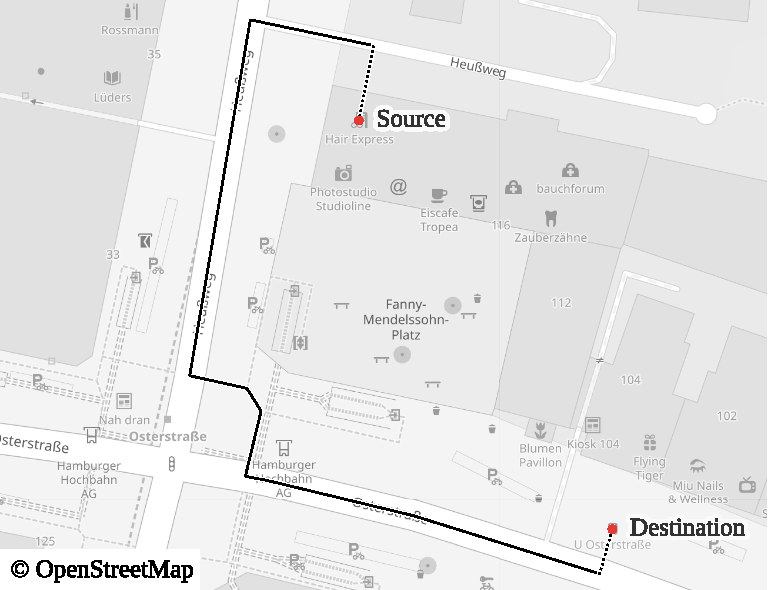
\includegraphics[width=0.65\textwidth]{images/qgis-routing-osterstrasse_routing.pdf}
				\end{figcenter}
				\caption{Graph-based routing result using \href{https://www.osm.org/directions?engine=graphhopper\_foot\&route=53.57657,9.95210;53.57601,9.95268}{\emph{GraphHopper}}.}
			\end{figure}
		\end{frame}
		
		\begin{frame}{Example: Expected routing behavior}
			\begin{figure}[t]
				\begin{figcenter}
					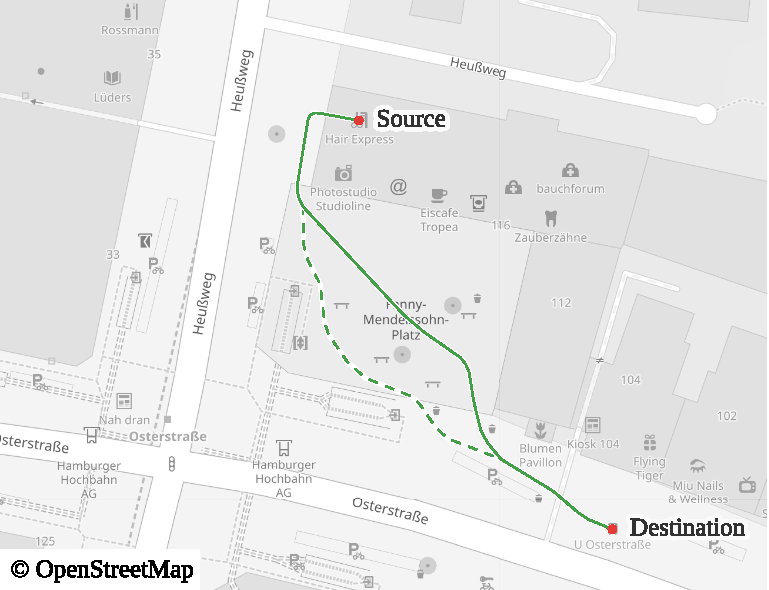
\includegraphics[width=0.65\textwidth]{images/qgis-routing-osterstrasse_expected.pdf}
				\end{figcenter}
				\caption{Routes an actual pedestrian would likely choose.}
			\end{figure}
		\end{frame}
		
%		\begin{frame}{Example 2: Densely built-up areas}
%			\begin{figure}[t]
%				\begin{figcenter}
%					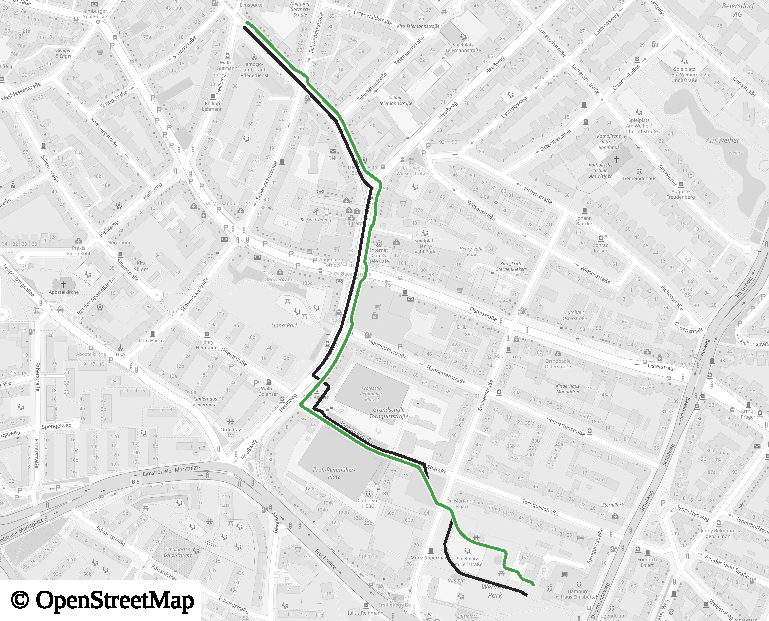
\includegraphics[width=0.65\textwidth]{images/qgis-routing-similar.pdf}
%				\end{figcenter}
%				\caption{Expected routes often follow graph edges, which hold valuable information.}
%			\end{figure}
%		\end{frame}
		
		\begin{frame}{Value of graph data}
			Graph data is still valuable:\n
			\begin{itemize}
				\item detailed information
				\begin{itemize}
					\item surface conditions, access restrictions, allowed vehicle types
				\end{itemize}
				\item definitely walkable
				\begin{itemize}
					\item no real-world obstacles in the way
				\end{itemize}
				\item sometimes without alternatives
				\begin{itemize}
					\item bridges, tunnels
					\item paths through obstacles (e.g. building passages)
				\end{itemize}
			\end{itemize}
		\end{frame}
	
	\section{Design}
	
		\begin{frame}{Wanted routing algorithm}
			Should be able to\n
			\begin{itemize}
				\item traverse open spaces\ \textrightarrow\ reach arbitrary locations
				\item use roads and ways
				\item create more realistic routes than purely graph-based routing
			\end{itemize}
			\nn
			\pause
			Additional requirements:\n
			\begin{itemize}
				\item based on C\# / .NET and MARS (Multi-Agent Research and Simulation)
				\item low impact on simulation time
			\end{itemize}
		\end{frame}
		
		\begin{frame}{Design decisions}
			Decisions of implemented algorithm:\n
			\begin{itemize}
				\item visibility graph generation
				\item merge with existing road network
				\item connect source / destination with visibility edges
				\item usage of graph-based routing
			\end{itemize}
			\nn
			\pause
			Alternative approaches:\n
			\begin{itemize}
				\item alternating routing with continuous Dijkstra
				\item merge of route segments in postprocessing step
				\item other graph-generation methods
				\begin{itemize}
					\item Voronoi diagrams, skeletonization
					\item ad-hoc generation (e.g. by using continuous Dijkstra)
				\end{itemize}
			\end{itemize}
		\end{frame}
		
		\begin{frame}{Components}
			\begin{figure}[t]
				\begin{figcenter}
					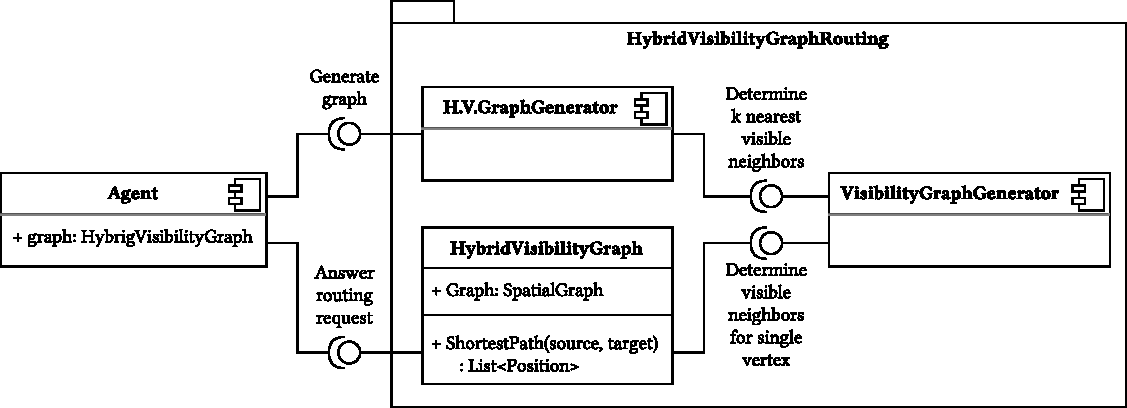
\includegraphics[width=0.95\textwidth]{images/components.pdf}
				\end{figcenter}
				\caption{Components of the implemented hybrid routing algorithm.}
			\end{figure}
		\end{frame}
		
		\begin{frame}{Graph generation}
			\begin{figure}[t]
				\begin{figcenter}
					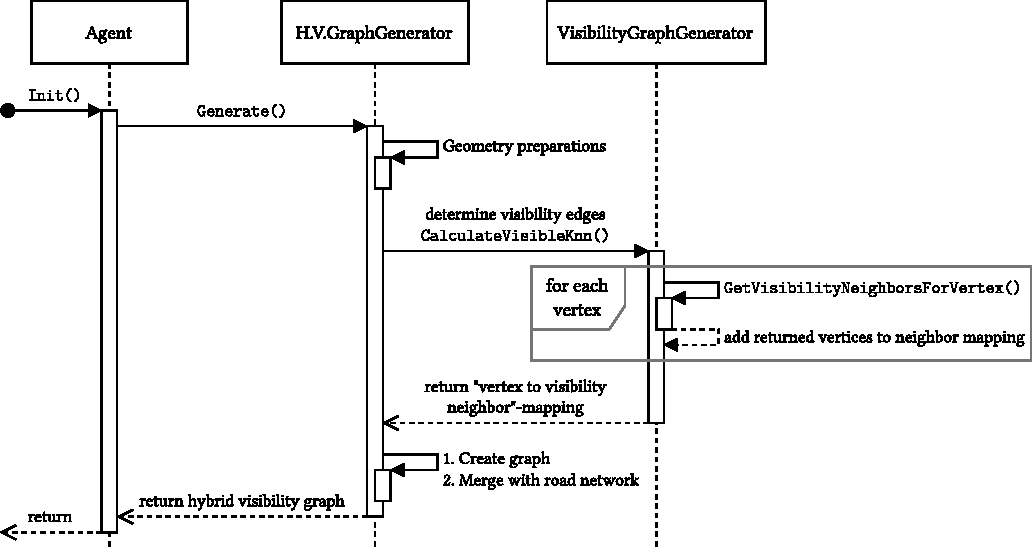
\includegraphics[width=0.98\textwidth]{images/components-sequence-generation-short.pdf}
				\end{figcenter}
				\caption{Separate steps of the graph generation.}
			\end{figure}
		\end{frame}
		
		\begin{frame}{Routing}
			\begin{figure}[t]
				\begin{figcenter}
					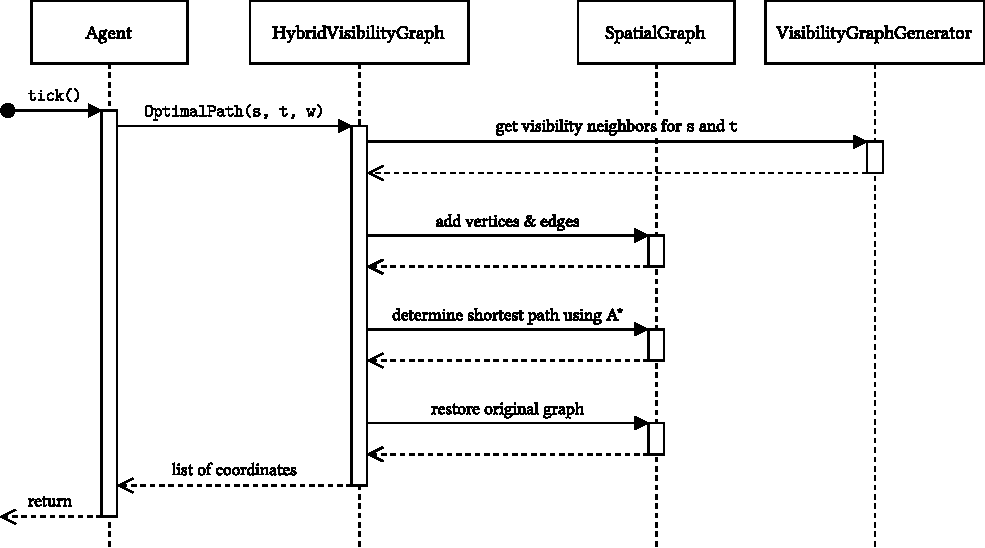
\includegraphics[width=0.95\textwidth]{images/components-sequence-routing-short.pdf}
				\end{figcenter}
				\caption{Separate steps of answering a routing request.}
			\end{figure}
		\end{frame}
	
	\section{Implementation}
	
		\begin{frame}{Considerations and terminology}
			Key considerations:\n
			\begin{itemize}
				\item custom implementation that supports
				\begin{itemize}
					\item collinear vertices
					\item arbitrary obstacle geometries (especially lines and polygons)
					\item intersecting obstacles
					\item arbitrary positions and non-unique coordinates
				\end{itemize}
				\item generate and connect nodes suitable for routing
			\end{itemize}
			\nn
			\pause
			Terminology:\n
			\begin{description}[visibility neighbor]
				\item[obstacle neighbor] vertex on same or touching obstacle
				\item[visibility neighbor] vertex across open space that is visible
				\item[input vertex] vertex / coordinate in the input dataset
				\item[output vertex] generated vertex in the visibility graph
			\end{description}
		\end{frame}
		
		\begin{frame}{Preparations}
			Before visibility graph is created:\n
			\begin{itemize}
				\item get obstacles from input data
				\item unwrap multi-geometries
				\item triangulate polygonal obstacles
				\begin{itemize}
					\item[\textrightarrow] performance optimization
				\end{itemize}
			\end{itemize}
		\end{frame}
		
		\begin{frame}{Visibility graph creation}
			\begin{enumerate}
				\item get obstacles from input data
				\item obtain data for visibility graph
				\begin{enumerate}
					\item for each vertex: determine its visibility neighbors
					\item sort visibility neighbors into bins based on obstacle neighbors
				\end{enumerate}
				\item generate routable visibility graph
				\item merge road edges
			\end{enumerate}
		\end{frame}
		
		\begin{frame}{Visibility graph creation: vertex and edge creation}
			Naive approach:
			\begin{itemize}
				\item one vertex per input coordinate
				\item routing through line-based obstacles possible
			\end{itemize}
			\nn
			\pause
			Correct approach:
			\begin{itemize}
				\item one vertex between adjacent obstacle neighbors
				\item multiple vertices at same location
				\item vertices are not connected
				\item routing through obstacle not possible
			\end{itemize}
		\end{frame}
	
		\begin{frame}{Visibility graph creation: vertex and edge creation}
			\begin{figure}
				\begin{figcenter}
					\scalebox{0.7}
					{
						\begin{tikzpicture}
	\def\d{0.03}
	
	\tikzDot[label=below:$v$]{(0,0)}{v}
	
	\tikzDot[label=left:$n_1$]{(-2.25,0)}{n1}
	\tikzDot[label=above:$n_2$]{(0,2)}{n2}
	\tikzDot[label=right:$n_3$]{(2.25,0)}{n3}
	
	\draw[lightgray] (v) -- (n1);
	\draw[lightgray] (v) -- (n3);
	\draw[lightgray] (v) -- (n2);
	
	% Visibility edges to n1
	\tikzDot[DodgerBlue3]{(-1.1,-0.25)}{vn1}
	\tikzDot[DodgerBlue3]{(-1.6,-0.9)}{vn2}
	\tikzDot[DodgerBlue3]{(1.6,-0.5)}{vn3}
	\draw[DodgerBlue3,densely dashed,->] (v) -- (vn1);
	\draw[DodgerBlue3,densely dashed,->] (v) -- (vn2);
	\draw[DodgerBlue3,densely dashed,->] (v) -- (vn3);
	
	% Visibility edges to n3
	\tikzDot[Red2]{(0.7,1.4)}{vn4}
	\tikzDot[Red2]{(2,1)}{vn5}
	\draw[Red2,densely dotted,->] (v) -- (vn4);
	\draw[Red2,densely dotted,->] (v) -- (vn5);
	
	% Visibility edges to n2
	\tikzDot[Green4]{(-2,1.3)}{vn6}
	\draw[Green4,dashdotted,->] (v) -- (vn6);
\end{tikzpicture}
					}
				\end{figcenter}
				\caption{Sorting visibility neighbors into bins, based on the obstacle neighbors of $v$.}
			\end{figure}
			\pause
			\begin{figure}
				\begin{figcenter}
					\scalebox{0.7}
					{
						\begin{tikzpicture}
	\tikzDot{(2,0)}{vo0};
	\tikzDot[label={[label distance=-1.25mm]above right:$v $}]{(2,1)}{vo1};
	\tikzDot{(2,2)}{vo2};
	
	\draw (vo0) -- (vo1);
	\draw (vo1) -- (vo2);
	
	\tikzDot[label=left:$n_a$,outer sep=0.5mm]{(0.5,1.3)}{n1};
	\tikzDot[label=right:$n_b$,outer sep=0.5mm]{(3.5,1)}{n2};
	
	\draw[dotted] (n1) -- (vo1);
	\draw[dotted] (vo1) -- (n2);
	
	\draw[dotted] (n1) -- (vo0);
	\draw[dotted] (n1) -- (vo2);
	\draw[dotted] (n2) -- (vo0);
	\draw[dotted] (n2) -- (vo2);
\end{tikzpicture}
					}
					\hspace{0.75cm}
					\scalebox{0.7}
					{
						\begin{tikzpicture}
	\def\r{0.85mm}
	\def\rMargin{1.1mm} % = r + 0.25mm
	\def\gap{0.1875mm}
	
	\tikzDot{(2,0)}{vo0};
	\node (vo1) at (2,1) {};
	\node[label={[label distance=-1.25mm]above left:$v_a$}] at (vo1) {};
	\node[label={[label distance=-1.25mm]above right:$v_b$}] at (vo1) {};
	\coordinate (vo11) at ($(vo1)+(180:\rMargin)$);
	\coordinate (vo12) at ($(vo1)+(0:\rMargin)$);
	\tikzDot{(2,2)}{vo2};
	
	\filldraw (vo1)++(-\gap,0)++(90:\r) arc (90:270:\r);
	\filldraw (vo1)++( \gap,0)++(90:\r) arc (90:-90:\r);
	
	\draw ($(vo1)+(270:\r)+(-0.275mm,0)$) -- ($(vo0)+(-0.275mm,2mm)$) -- (vo0.north);
	\draw ($(vo1)+(270:\r)+( 0.275mm,0)$) -- ($(vo0)+( 0.275mm,2mm)$) -- (vo0.north);
	
	\draw ($(vo1)+(90:\r)+(-0.275mm,0)$) -- ($(vo2)+(-0.275mm,-2mm)$) -- (vo2.south);
	\draw ($(vo1)+(90:\r)+( 0.275mm,0)$) -- ($(vo2)+( 0.275mm,-2mm)$) -- (vo2.south);
	
	\tikzDot[label=left:$n_a$,outer sep=0.5mm]{(0.5,1.3)}{n1};
	\tikzDot[label=right:$n_b$,outer sep=0.5mm]{(3.5,1)}{n2};
	
	\draw[dotted] (n1) -- (vo11);
	\draw[dotted] (vo12) -- (n2);
	
	\draw[dotted] (n1) -- (vo0);
	\draw[dotted] (n1) -- (vo2);
	\draw[dotted] (n2) -- (vo0);
	\draw[dotted] (n2) -- (vo2);
\end{tikzpicture}
					}
				\end{figcenter}
				\caption{Naive (left) and correct (right) vertex creation and connection.}
			\end{figure}
		\end{frame}
		
		\begin{frame}{Road network merge}
			\begin{enumerate}
				\item create vertices at intersection points
				\item connect new vertex
				\item remove old edges
			\end{enumerate}
			\begin{figure}
				\begin{figcenter}
					\scalebox{0.7}
					{
						\begin{tikzpicture}
	\tikzDot{(0,-0.75)}{v1n1}
	\tikzDot{(4,-0.6)}{v1n2}
	
	\tikzDot{(0,0.8)}{v2n1}
	\tikzDot{(4.2,0.6)}{v2n2}
	
	\tikzDot{(1.5,-1.65)}{rn1}
	\tikzDot{(1.8,1.65)}{rn2}
	
	\draw[<->,dashed] (v1n1) -- node[above right=0cm and 0.4cm] {$v$} (v1n2);
	\draw[<->,dashed] (v2n1) -- node[above right=0cm and 0.4cm] {$u$} (v2n2);
	
	\draw[<->] (rn1) -- node[left] {$r$} (rn2);
\end{tikzpicture}
					}
					\hspace{0.75cm}
					\scalebox{0.7}
					{
						\begin{tikzpicture}
	\tikzDot{(0,-0.75)}{v1n1}
	\tikzDot{(4,-0.6)}{v1n2}
	
	\tikzDot{(0,0.8)}{v2n1}
	\tikzDot{(4.2,0.6)}{v2n2}
	
	\tikzDot{(1.5,-1.65)}{rn1}
	\tikzDot{(1.8,1.65)}{rn2}
	
	\tikzDot{(intersection of v1n1--v1n2 and rn1--rn2)}{i1}
	\tikzDot{(intersection of v2n1--v2n2 and rn1--rn2)}{i2}
	
	\draw[<->,dashed] (v1n1) -- node[above] {$v_1$} (i1);
	\draw[<->,dashed] (i1)   -- node[above] {$v_2$} (v1n2);
	\draw[<->,dashed] (v2n1) -- node[above] {$u_1$} (i2);
	\draw[<->,dashed] (i2)   -- node[above] {$u_2$} (v2n2);
	
	\draw[<->] (rn1) -- node[right] {$r_1$} (i1);
	\draw[<->] (i1)  -- node[right] {$r_2$} (i2);
	\draw[<->] (i2)  -- node[right] {$r_3$} (rn2);
\end{tikzpicture}
					}
				\end{figcenter}
				\caption{Merge of road network and visibility edges.}
			\end{figure}
		\end{frame}
		
		\begin{frame}{Answering routing queries}
			\begin{enumerate}
				\item add vertices for source \& destination to graph
				\item create and add their visibility edges
				\begin{itemize}
					\item[\textrightarrow] same algorithm used for graph generation
				\end{itemize}
				\item use A* to determine shortest path
				\item remove previously created vertices and edges
			\end{enumerate}
		\end{frame}
		
		\begin{frame}{Performance optimizations}
			Only consider $k = k_b \cdot k_n$ many visibility neighbors:
			\begin{itemize}
				\item ensure neighbors exist in all directions
				\item $k_b$ bins, each covering $360 / k_b$ degree
				\item $k_n$ neighbors per bin
			\end{itemize}
			\nn
			\pause
			Only consider vertices on a convex hull:\n
			\begin{itemize}
				\item convex hull is shortest path around polygon
				\item[\textrightarrow\hspace{-0.1cm}] vertex not on any convex hull will never be part of any shortest path
			\end{itemize}
		\end{frame}
		
		\begin{frame}{Performance optimizations}
			Only consider potential visibility neighbors at certain angles:\n
			\begin{itemize}
				\item consider shortest path $p$\ \textrightarrow\ no edges can be relaxed
				\item only vertices at certain angles are valid neighbors\ \textrightarrow\ valid angle area
			\end{itemize}
			\pause
			\begin{figure}[b]
				\begin{figcenter}
					\scalebox{0.7}
					{
						\begin{tikzpicture}
	\coordinate (c00) at (0,0.4);
	\draw (c00)
	-- ++(2.75,-0.2) coordinate (c01)
	-- ++(0.8,0.4) coordinate (c02)
	-- ++(0.1,0.8) coordinate (c03)
	-- ++(-2,0) coordinate (c04)
	-- ++(-1.4,-0.35) coordinate (c05)
	-- (c00);
	\node[above right = 0.15 and 1.6 of c00] {$o_1$};
	
	\coordinate (c10) at (2.5,3.85);
	\draw (c10)
	-- ++(-0.4,-0.4) coordinate (c11)
	-- ++(0.1,-0.6) coordinate (c12)
	-- ++(2.8,0) coordinate (c13)
	-- ++(-0.4,1.2) coordinate (c14)
	-- (c10);
	\node[below right = 0.25 and 0.75 of c10] {$o_2$};
	
	\def\d{1.5\pgflinewidth}
	\filldraw[line width=0,Green4!35!white]
	($(c03)+(0,\d)$) --
	+(180:0.35) arc [start angle=180, delta angle=-97.126, radius=0.35];
	\draw[thin,Green4] (c03) -- (intersection of c03--[shift=(c03)]82.874:3 and c12--c13);
	\draw[thin,Green4] ($(c03)+(0,\d)$) -- +(180:4);
	
	\filldraw[line width=0,DodgerBlue3!35!white]
	($(c12)+(0,-\d)$) --
	+(279.462:0.4) arc [start angle=279.462, delta angle=80.538, radius=0.4];
	\draw[thin,DodgerBlue3] (c12) -- (intersection of c12--[shift=(c12)]279.462:1 and c03--c04);
	\draw[thin,DodgerBlue3] ($(c12)+(0,-\d)$) -- +(0:4);
	
	\tikzDot[label={right:$s$}]{(c01)}{s}
	\tikzDot[label={right:$v_0$}]{(c02)}{v0}
	\tikzDot[label={right:$v_1$}]{(c03)}{v1}
	\tikzDot[label={left:$v_2$}]{(c12)}{v2}
	\tikzDot[label={below:$v_3$}]{(c13)}{v3}
	\tikzDot[label={above:$v_4$}]{(c04)}{v4}
	\tikzDot[label={left:$t$}]{(c10)}{t}
	
	\draw[->,Red2,thick] (s) -- (v0);
	\draw[->,Red2,thick] (v0) -- (v1);
	\draw[->,Red2,thick] (v1) -- (v2);
	\draw[->,Red2,thick] (v2) -- (c11);
	\draw[->,Red2,thick] (c11) -- (t);
\end{tikzpicture}

					}
				\end{figcenter}
				\caption{Valid angle areas (blue and green).}
			\end{figure}
		\end{frame}
		
		\begin{frame}{Performance optimizations}
			Exclude vertices in \enquote{shadow} of obstacles:\n
			\begin{itemize}
				\item consider vertex $v$ and think of it as light bulb
				\item obstacles cast shadow outwards, hiding vertices
			\end{itemize}
			\pause
			\begin{figure}[b]
				\begin{figcenter}
					\scalebox{0.7}
					{
						\begin{tikzpicture}
	\def\angle{20}
	\def\boundingVertexDistance{3}
	
	\tikzDot[label=$v$]{(0,1.5)}{v}
	\coordinate (shadow-arc-top)				at ($(v) +( \angle:\boundingVertexDistance)$);
	\coordinate (shadow-arc-bottom)				at ($(v) +(-\angle:\boundingVertexDistance)$);
	\coordinate (shadow-arc-top-end)			at ($(v) +( \angle:5.75)$);
	\coordinate (shadow-arc-bottom-end)			at ($(v) +(-\angle:5.75)$);
	\coordinate (shadow-arc-top-faded-end)		at ($(v) +( \angle:6.5)$);
	\coordinate (shadow-arc-bottom-faded-end)	at ($(v) +(-\angle:6.5)$);
	
	% Gray area
	\filldraw[lightgray] 
	(shadow-arc-bottom) arc [start angle=-\angle, delta angle=2*\angle, radius=\boundingVertexDistance] --
	(shadow-arc-top-end) --
	(shadow-arc-bottom-end) --
	cycle;
	\draw[gray]
	(shadow-arc-bottom-end) --
	(shadow-arc-bottom) arc [start angle=-\angle, delta angle=2*\angle, radius=\boundingVertexDistance] --
	(shadow-arc-top-end);
	
	\draw[dotted] (v) -- (shadow-arc-top);
	\draw[dotted] (v) -- (shadow-arc-bottom);
	
	% Faded gray area
	\filldraw[draw=none,lightgray,path fading=east]
	(shadow-arc-top-faded-end) --
	(shadow-arc-top-end) --
	(shadow-arc-bottom-end) --
	(shadow-arc-bottom-faded-end) --
	cycle;
	\draw[gray,path fading=east] (shadow-arc-top-end) -- (shadow-arc-top-faded-end);
	\draw[gray,path fading=east] (shadow-arc-bottom-end) -- (shadow-arc-bottom-faded-end);
	
	% Obstacle
	\tikzDot[Red2]{(shadow-arc-top)}{o0}
	\tikzDot{(3.8,2)}{o1}
	\tikzDot[Red2]{($(v) +(-\angle:1.2)$)}{o2}
	\node[above right = 0.5 and 1.15 of o2] {$o$};
	
	% v' and v''
	\tikzDot[label=right:$v'$]{(2.1,1.1)}{v'}
	\tikzDot[label=right:$v''$]{(3.4,1.3)}{v''}
	
	\node[darkgray] at (4.7,1.5) {\huge$S$};
	
	\draw (o0) -- (o1) -- (o2) -- (o0);
\end{tikzpicture}

					}
				\end{figcenter}
				\caption{Shadow area $S$ cast by obstacle $o$.}
			\end{figure}
		\end{frame}
		
		\begin{frame}{Performance optimizations}
			Interval data structure for shadow areas:\n
			\begin{itemize}
				\item bin-based: each bin covers certain angle interval
				\item constant-time bin access
			\end{itemize}
			\begin{figure}[b]
				\begin{figcenter}
					\scalebox{0.7}
					{
						
\begin{tikzpicture}
	\def\l{0.5}
	\def\countX{9} % One more is added due to start at x=0
	\def\countY{1} % One more is added due to start at x=0
	
	\def\itemBStartX{1.6}
	\def\itemBIndexStart{1}
	\def\itemBLength{4.1}
	
	\def\itemAStartX{4}
	\def\itemAIndexStart{4}
	\def\itemALength{7.8}
	
	% Item A: Bins 1-5
	\draw[dotted,gray] (\itemBStartX*\l, \countY+4*\l) -- +(0, -\countY-4*\l);
	\draw[dotted,gray] (\itemBStartX*\l+\itemBLength*\l, \countY+4*\l) -- +(0, -\countY-4*\l);
	\filldraw[preaction={fill, white},pattern=north west lines,pattern color=Red2] (\itemBStartX*\l,\countY+4*\l) rectangle node[above right=0.125 and -1.3]{Item B: \itemBStartX\ - 5.7} ++(\itemBLength*\l,0.5*\l);
	
	% Item B: Bins 4-11(2)
	\draw[dotted,gray] (\itemAStartX*\l, \countY+3*\l) -- +(0, -\countY-3*\l);
	\draw[dotted,gray] (\itemAStartX*\l+\itemALength*\l, \countY+3*\l) -- +(0, -\countY-3*\l);
	\filldraw[preaction={fill, white},pattern=crosshatch dots,pattern color=DodgerBlue3] (\itemAStartX*\l,\countY+3*\l) rectangle node[above right=0.125 and -0.5]{Item A: \itemAStartX\ - 10.8} ++(\itemALength*\l,0.5*\l);
	
	\draw[->] (\itemAStartX*\l+1.85,\countY+2.75*\l) -- node[right] {1.} +(0,-1.5*\l);
	\draw[->] (\itemBStartX*\l+0.5,\countY+3.75*\l) -- node[right] {2.} +(0,-2.5*\l);
	
	% Draw pattern to bins
	\fill[preaction={fill, white},pattern=north west lines,pattern color=Red2] (\itemBIndexStart*\l,1.5*\l) rectangle ++(\l,\l);
	\fill[preaction={fill, white},pattern=north west lines,pattern color=Red2] (\itemBIndexStart*\l+1*\l,0) rectangle ++(2*\l,\l);
	\fill[preaction={fill, white},pattern=north west lines,pattern color=Red2] (\itemBIndexStart*\l+3*\l,1.5*\l) rectangle ++(\l,\l);
	\fill[preaction={fill, white},pattern=north west lines,pattern color=Red2] (\itemBIndexStart*\l+4*\l,1.5*\l) rectangle ++(\l,\l);
	
	\fill[preaction={fill, white},pattern=crosshatch dots,pattern color=DodgerBlue3] (\itemAIndexStart*\l,0) rectangle ++(6*\l,\l);
	\fill[preaction={fill, white},pattern=crosshatch dots,pattern color=DodgerBlue3] (0,0) rectangle ++(2*\l,\l);
	
	% Draw gray versions of filled bins
	\fill[preaction={fill, white},pattern=north west lines,pattern color=lightgray] (\l*\countX+\l+\itemBIndexStart*\l+1*\l,0) rectangle ++(\l,\l);
	\fill[preaction={fill, white},pattern=crosshatch dots,pattern color=lightgray] (\l*\countX+\l,0) rectangle ++(2*\l,\l);
	
	% Draw outlines of repeating gray bins
	\foreach \x in {0,...,2}
	{
		\draw[lightgray] (\l*\countX+\l+\l*\x,0) rectangle ++(\l,\l);
		\node[lightgray] at (\l*\countX+\l+\l*\x+0.5*\l,-0.35) {$\x$};
	}
	
	% Draw outlines of bins
	\foreach \x in {0,...,\countX}
	{
		\draw (\l*\x,0) rectangle ++(\l,\l);
		\node at (\l*\x+0.5*\l,-0.35) {$\x$};
	}
	
	\draw (\itemBIndexStart*\l,1.5*\l) rectangle ++(\l,\l);
	\draw[->] (\itemBIndexStart*\l+0.5*\l,\l) -- ++(0,0.5*\l);
	
	\draw (\itemBIndexStart*\l+3*\l,1.5*\l) rectangle ++(\l,\l);
	\draw[->] (\itemBIndexStart*\l+3.5*\l,\l) -- ++(0,0.5*\l);
	
	\draw (\itemBIndexStart*\l+4*\l,1.5*\l) rectangle ++(\l,\l);
	\draw[->] (\itemBIndexStart*\l+4.5*\l,\l) -- ++(0,0.5*\l);
	
	\node at (0.5*\countX*\l,-0.875) {bins};
	\node[align=right] at (-1.25,0.5*\countY*\l+0.5*\l) {Linked lists\\of bins};
\end{tikzpicture}
					}
				\end{figcenter}
				\caption{BinIndex data structure storing two overlapping intervals.}
			\end{figure}
		\end{frame}
		
		\begin{frame}{Performance optimizations}
			Additional optimizations:
			\begin{itemize}
				\item usage of spatial indices
				\item custom line segment intersection check
				\item custom triangle intersection check
			\end{itemize}
		\end{frame}
	
	\section{Evaluation}
	
		\begin{frame}{Optimization impact}
			\begin{table}
				\begin{tabularx}{0.8\textwidth}{p{4.25cm}RR}
\toprule
\textbf{Enabled optimization}	& \textbf{Time}	& \textbf{Speedup}	\\
\midrule
Shadow areas					&  22.2 s		& 35.56				\\
kNN filtering					& 751.7 s		&  1.05				\\
Vertices on convex hull			& 287.9 s		&  2.74				\\
Valid angle areas				& 322.5 s		&  2.44				\\
Custom collision detection		& 769.3 s		&  1.02				\\
\midrule
No active optimization			& 788.5 s		&  1.00				\\
All optimizations active		&  11.1 s		& 71.13				\\
\bottomrule
				\end{tabularx}
				\caption{Impact of optimizations on the graph generation using the 0.5 km\textsuperscript{2} \enquote{OSM city} dataset.}
				\label{table:optimization-impact}
			\end{table}
		\end{frame}
		
		\begin{frame}{Graph generation task performance}
			\begin{figure}
				\begin{figcenter}
					\hspace*{-0.35cm}
					\scalebox{0.7}
					{
						%% Creator: Matplotlib, PGF backend
%%
%% To include the figure in your LaTeX document, write
%%   \input{<filename>.pgf}
%%
%% Make sure the required packages are loaded in your preamble
%%   \usepackage{pgf}
%%
%% Also ensure that all the required font packages are loaded; for instance,
%% the lmodern package is sometimes necessary when using math font.
%%   \usepackage{lmodern}
%%
%% Figures using additional raster images can only be included by \input if
%% they are in the same directory as the main LaTeX file. For loading figures
%% from other directories you can use the `import` package
%%   \usepackage{import}
%%
%% and then include the figures with
%%   \import{<path to file>}{<filename>.pgf}
%%
%% Matplotlib used the following preamble
%%   
%%   \usepackage{fontspec}
%%   \setmainfont{DejaVuSerif.ttf}[Path=\detokenize{/home/hauke/.local/lib/python3.11/site-packages/matplotlib/mpl-data/fonts/ttf/}]
%%   \setsansfont{DroidSans.ttf}[Path=\detokenize{/usr/share/fonts/droid/}]
%%   \setmonofont{DejaVuSansMono.ttf}[Path=\detokenize{/home/hauke/.local/lib/python3.11/site-packages/matplotlib/mpl-data/fonts/ttf/}]
%%   \makeatletter\@ifpackageloaded{underscore}{}{\usepackage[strings]{underscore}}\makeatother
%%
\begingroup%
\makeatletter%
\begin{pgfpicture}%
\pgfpathrectangle{\pgfpointorigin}{\pgfqpoint{6.101690in}{1.716449in}}%
\pgfusepath{use as bounding box, clip}%
\begin{pgfscope}%
\pgfsetbuttcap%
\pgfsetmiterjoin%
\definecolor{currentfill}{rgb}{1.000000,1.000000,1.000000}%
\pgfsetfillcolor{currentfill}%
\pgfsetlinewidth{0.000000pt}%
\definecolor{currentstroke}{rgb}{1.000000,1.000000,1.000000}%
\pgfsetstrokecolor{currentstroke}%
\pgfsetdash{}{0pt}%
\pgfpathmoveto{\pgfqpoint{0.000000in}{0.000000in}}%
\pgfpathlineto{\pgfqpoint{6.101690in}{0.000000in}}%
\pgfpathlineto{\pgfqpoint{6.101690in}{1.716449in}}%
\pgfpathlineto{\pgfqpoint{0.000000in}{1.716449in}}%
\pgfpathlineto{\pgfqpoint{0.000000in}{0.000000in}}%
\pgfpathclose%
\pgfusepath{fill}%
\end{pgfscope}%
\begin{pgfscope}%
\pgfsetbuttcap%
\pgfsetmiterjoin%
\definecolor{currentfill}{rgb}{1.000000,1.000000,1.000000}%
\pgfsetfillcolor{currentfill}%
\pgfsetlinewidth{0.000000pt}%
\definecolor{currentstroke}{rgb}{0.000000,0.000000,0.000000}%
\pgfsetstrokecolor{currentstroke}%
\pgfsetstrokeopacity{0.000000}%
\pgfsetdash{}{0pt}%
\pgfpathmoveto{\pgfqpoint{0.592976in}{0.400938in}}%
\pgfpathlineto{\pgfqpoint{4.765159in}{0.400938in}}%
\pgfpathlineto{\pgfqpoint{4.765159in}{1.716449in}}%
\pgfpathlineto{\pgfqpoint{0.592976in}{1.716449in}}%
\pgfpathlineto{\pgfqpoint{0.592976in}{0.400938in}}%
\pgfpathclose%
\pgfusepath{fill}%
\end{pgfscope}%
\begin{pgfscope}%
\definecolor{textcolor}{rgb}{0.150000,0.150000,0.150000}%
\pgfsetstrokecolor{textcolor}%
\pgfsetfillcolor{textcolor}%
\pgftext[x=0.940658in,y=0.268994in,,top]{\color{textcolor}\sffamily\fontsize{9.000000}{10.800000}\selectfont Total time}%
\end{pgfscope}%
\begin{pgfscope}%
\definecolor{textcolor}{rgb}{0.150000,0.150000,0.150000}%
\pgfsetstrokecolor{textcolor}%
\pgfsetfillcolor{textcolor}%
\pgftext[x=1.636022in,y=0.268994in,,top]{\color{textcolor}\sffamily\fontsize{9.000000}{10.800000}\selectfont kNN search}%
\end{pgfscope}%
\begin{pgfscope}%
\definecolor{textcolor}{rgb}{0.150000,0.150000,0.150000}%
\pgfsetstrokecolor{textcolor}%
\pgfsetfillcolor{textcolor}%
\pgftext[x=2.147517in, y=0.174023in, left, base]{\color{textcolor}\sffamily\fontsize{9.000000}{10.800000}\selectfont Create}%
\end{pgfscope}%
\begin{pgfscope}%
\definecolor{textcolor}{rgb}{0.150000,0.150000,0.150000}%
\pgfsetstrokecolor{textcolor}%
\pgfsetfillcolor{textcolor}%
\pgftext[x=2.168086in, y=0.030029in, left, base]{\color{textcolor}\sffamily\fontsize{9.000000}{10.800000}\selectfont graph}%
\end{pgfscope}%
\begin{pgfscope}%
\definecolor{textcolor}{rgb}{0.150000,0.150000,0.150000}%
\pgfsetstrokecolor{textcolor}%
\pgfsetfillcolor{textcolor}%
\pgftext[x=2.929002in, y=0.174023in, left, base]{\color{textcolor}\sffamily\fontsize{9.000000}{10.800000}\selectfont Get}%
\end{pgfscope}%
\begin{pgfscope}%
\definecolor{textcolor}{rgb}{0.150000,0.150000,0.150000}%
\pgfsetstrokecolor{textcolor}%
\pgfsetfillcolor{textcolor}%
\pgftext[x=2.764756in, y=0.030029in, left, base]{\color{textcolor}\sffamily\fontsize{9.000000}{10.800000}\selectfont obstacles}%
\end{pgfscope}%
\begin{pgfscope}%
\definecolor{textcolor}{rgb}{0.150000,0.150000,0.150000}%
\pgfsetstrokecolor{textcolor}%
\pgfsetfillcolor{textcolor}%
\pgftext[x=3.397101in, y=0.174023in, left, base]{\color{textcolor}\sffamily\fontsize{9.000000}{10.800000}\selectfont Merge road}%
\end{pgfscope}%
\begin{pgfscope}%
\definecolor{textcolor}{rgb}{0.150000,0.150000,0.150000}%
\pgfsetstrokecolor{textcolor}%
\pgfsetfillcolor{textcolor}%
\pgftext[x=3.558020in, y=0.030029in, left, base]{\color{textcolor}\sffamily\fontsize{9.000000}{10.800000}\selectfont edges}%
\end{pgfscope}%
\begin{pgfscope}%
\definecolor{textcolor}{rgb}{0.150000,0.150000,0.150000}%
\pgfsetstrokecolor{textcolor}%
\pgfsetfillcolor{textcolor}%
\pgftext[x=4.187039in, y=0.174023in, left, base]{\color{textcolor}\sffamily\fontsize{9.000000}{10.800000}\selectfont Add POI}%
\end{pgfscope}%
\begin{pgfscope}%
\definecolor{textcolor}{rgb}{0.150000,0.150000,0.150000}%
\pgfsetstrokecolor{textcolor}%
\pgfsetfillcolor{textcolor}%
\pgftext[x=4.143979in, y=0.030029in, left, base]{\color{textcolor}\sffamily\fontsize{9.000000}{10.800000}\selectfont attributes}%
\end{pgfscope}%
\begin{pgfscope}%
\pgfpathrectangle{\pgfqpoint{0.592976in}{0.400938in}}{\pgfqpoint{4.172183in}{1.315510in}}%
\pgfusepath{clip}%
\pgfsetroundcap%
\pgfsetroundjoin%
\pgfsetlinewidth{1.003750pt}%
\definecolor{currentstroke}{rgb}{0.800000,0.800000,0.800000}%
\pgfsetstrokecolor{currentstroke}%
\pgfsetdash{}{0pt}%
\pgfpathmoveto{\pgfqpoint{0.592976in}{0.628876in}}%
\pgfpathlineto{\pgfqpoint{4.765159in}{0.628876in}}%
\pgfusepath{stroke}%
\end{pgfscope}%
\begin{pgfscope}%
\definecolor{textcolor}{rgb}{0.150000,0.150000,0.150000}%
\pgfsetstrokecolor{textcolor}%
\pgfsetfillcolor{textcolor}%
\pgftext[x=0.194444in, y=0.581391in, left, base]{\color{textcolor}\sffamily\fontsize{9.000000}{10.800000}\selectfont \(\displaystyle {10^{-4}}\)}%
\end{pgfscope}%
\begin{pgfscope}%
\pgfpathrectangle{\pgfqpoint{0.592976in}{0.400938in}}{\pgfqpoint{4.172183in}{1.315510in}}%
\pgfusepath{clip}%
\pgfsetroundcap%
\pgfsetroundjoin%
\pgfsetlinewidth{1.003750pt}%
\definecolor{currentstroke}{rgb}{0.800000,0.800000,0.800000}%
\pgfsetstrokecolor{currentstroke}%
\pgfsetdash{}{0pt}%
\pgfpathmoveto{\pgfqpoint{0.592976in}{1.014126in}}%
\pgfpathlineto{\pgfqpoint{4.765159in}{1.014126in}}%
\pgfusepath{stroke}%
\end{pgfscope}%
\begin{pgfscope}%
\definecolor{textcolor}{rgb}{0.150000,0.150000,0.150000}%
\pgfsetstrokecolor{textcolor}%
\pgfsetfillcolor{textcolor}%
\pgftext[x=0.194444in, y=0.966641in, left, base]{\color{textcolor}\sffamily\fontsize{9.000000}{10.800000}\selectfont \(\displaystyle {10^{-2}}\)}%
\end{pgfscope}%
\begin{pgfscope}%
\pgfpathrectangle{\pgfqpoint{0.592976in}{0.400938in}}{\pgfqpoint{4.172183in}{1.315510in}}%
\pgfusepath{clip}%
\pgfsetroundcap%
\pgfsetroundjoin%
\pgfsetlinewidth{1.003750pt}%
\definecolor{currentstroke}{rgb}{0.800000,0.800000,0.800000}%
\pgfsetstrokecolor{currentstroke}%
\pgfsetdash{}{0pt}%
\pgfpathmoveto{\pgfqpoint{0.592976in}{1.399377in}}%
\pgfpathlineto{\pgfqpoint{4.765159in}{1.399377in}}%
\pgfusepath{stroke}%
\end{pgfscope}%
\begin{pgfscope}%
\definecolor{textcolor}{rgb}{0.150000,0.150000,0.150000}%
\pgfsetstrokecolor{textcolor}%
\pgfsetfillcolor{textcolor}%
\pgftext[x=0.274690in, y=1.351892in, left, base]{\color{textcolor}\sffamily\fontsize{9.000000}{10.800000}\selectfont \(\displaystyle {10^{0}}\)}%
\end{pgfscope}%
\begin{pgfscope}%
\definecolor{textcolor}{rgb}{0.150000,0.150000,0.150000}%
\pgfsetstrokecolor{textcolor}%
\pgfsetfillcolor{textcolor}%
\pgftext[x=0.125000in,y=1.058693in,,bottom,rotate=90.000000]{\color{textcolor}\sffamily\fontsize{9.000000}{10.800000}\selectfont Time in s}%
\end{pgfscope}%
\begin{pgfscope}%
\pgfpathrectangle{\pgfqpoint{0.592976in}{0.400938in}}{\pgfqpoint{4.172183in}{1.315510in}}%
\pgfusepath{clip}%
\pgfsetbuttcap%
\pgfsetmiterjoin%
\definecolor{currentfill}{rgb}{0.349020,0.490196,0.749020}%
\pgfsetfillcolor{currentfill}%
\pgfsetlinewidth{1.003750pt}%
\definecolor{currentstroke}{rgb}{1.000000,1.000000,1.000000}%
\pgfsetstrokecolor{currentstroke}%
\pgfsetdash{}{0pt}%
\pgfpathmoveto{\pgfqpoint{0.662512in}{-191.225881in}}%
\pgfpathlineto{\pgfqpoint{0.847943in}{-191.225881in}}%
\pgfpathlineto{\pgfqpoint{0.847943in}{1.656653in}}%
\pgfpathlineto{\pgfqpoint{0.662512in}{1.656653in}}%
\pgfpathlineto{\pgfqpoint{0.662512in}{-191.225881in}}%
\pgfpathclose%
\pgfusepath{stroke,fill}%
\end{pgfscope}%
\begin{pgfscope}%
\pgfpathrectangle{\pgfqpoint{0.592976in}{0.400938in}}{\pgfqpoint{4.172183in}{1.315510in}}%
\pgfusepath{clip}%
\pgfsetbuttcap%
\pgfsetmiterjoin%
\definecolor{currentfill}{rgb}{0.349020,0.490196,0.749020}%
\pgfsetfillcolor{currentfill}%
\pgfsetlinewidth{1.003750pt}%
\definecolor{currentstroke}{rgb}{1.000000,1.000000,1.000000}%
\pgfsetstrokecolor{currentstroke}%
\pgfsetdash{}{0pt}%
\pgfpathmoveto{\pgfqpoint{1.357876in}{-191.225881in}}%
\pgfpathlineto{\pgfqpoint{1.543307in}{-191.225881in}}%
\pgfpathlineto{\pgfqpoint{1.543307in}{1.577437in}}%
\pgfpathlineto{\pgfqpoint{1.357876in}{1.577437in}}%
\pgfpathlineto{\pgfqpoint{1.357876in}{-191.225881in}}%
\pgfpathclose%
\pgfusepath{stroke,fill}%
\end{pgfscope}%
\begin{pgfscope}%
\pgfpathrectangle{\pgfqpoint{0.592976in}{0.400938in}}{\pgfqpoint{4.172183in}{1.315510in}}%
\pgfusepath{clip}%
\pgfsetbuttcap%
\pgfsetmiterjoin%
\definecolor{currentfill}{rgb}{0.349020,0.490196,0.749020}%
\pgfsetfillcolor{currentfill}%
\pgfsetlinewidth{1.003750pt}%
\definecolor{currentstroke}{rgb}{1.000000,1.000000,1.000000}%
\pgfsetstrokecolor{currentstroke}%
\pgfsetdash{}{0pt}%
\pgfpathmoveto{\pgfqpoint{2.053240in}{-191.225881in}}%
\pgfpathlineto{\pgfqpoint{2.238670in}{-191.225881in}}%
\pgfpathlineto{\pgfqpoint{2.238670in}{1.271553in}}%
\pgfpathlineto{\pgfqpoint{2.053240in}{1.271553in}}%
\pgfpathlineto{\pgfqpoint{2.053240in}{-191.225881in}}%
\pgfpathclose%
\pgfusepath{stroke,fill}%
\end{pgfscope}%
\begin{pgfscope}%
\pgfpathrectangle{\pgfqpoint{0.592976in}{0.400938in}}{\pgfqpoint{4.172183in}{1.315510in}}%
\pgfusepath{clip}%
\pgfsetbuttcap%
\pgfsetmiterjoin%
\definecolor{currentfill}{rgb}{0.349020,0.490196,0.749020}%
\pgfsetfillcolor{currentfill}%
\pgfsetlinewidth{1.003750pt}%
\definecolor{currentstroke}{rgb}{1.000000,1.000000,1.000000}%
\pgfsetstrokecolor{currentstroke}%
\pgfsetdash{}{0pt}%
\pgfpathmoveto{\pgfqpoint{2.748604in}{-191.225881in}}%
\pgfpathlineto{\pgfqpoint{2.934034in}{-191.225881in}}%
\pgfpathlineto{\pgfqpoint{2.934034in}{1.085627in}}%
\pgfpathlineto{\pgfqpoint{2.748604in}{1.085627in}}%
\pgfpathlineto{\pgfqpoint{2.748604in}{-191.225881in}}%
\pgfpathclose%
\pgfusepath{stroke,fill}%
\end{pgfscope}%
\begin{pgfscope}%
\pgfpathrectangle{\pgfqpoint{0.592976in}{0.400938in}}{\pgfqpoint{4.172183in}{1.315510in}}%
\pgfusepath{clip}%
\pgfsetbuttcap%
\pgfsetmiterjoin%
\definecolor{currentfill}{rgb}{0.349020,0.490196,0.749020}%
\pgfsetfillcolor{currentfill}%
\pgfsetlinewidth{1.003750pt}%
\definecolor{currentstroke}{rgb}{1.000000,1.000000,1.000000}%
\pgfsetstrokecolor{currentstroke}%
\pgfsetdash{}{0pt}%
\pgfpathmoveto{\pgfqpoint{3.443968in}{-191.225881in}}%
\pgfpathlineto{\pgfqpoint{3.629398in}{-191.225881in}}%
\pgfpathlineto{\pgfqpoint{3.629398in}{1.613652in}}%
\pgfpathlineto{\pgfqpoint{3.443968in}{1.613652in}}%
\pgfpathlineto{\pgfqpoint{3.443968in}{-191.225881in}}%
\pgfpathclose%
\pgfusepath{stroke,fill}%
\end{pgfscope}%
\begin{pgfscope}%
\pgfpathrectangle{\pgfqpoint{0.592976in}{0.400938in}}{\pgfqpoint{4.172183in}{1.315510in}}%
\pgfusepath{clip}%
\pgfsetbuttcap%
\pgfsetmiterjoin%
\definecolor{currentfill}{rgb}{0.349020,0.490196,0.749020}%
\pgfsetfillcolor{currentfill}%
\pgfsetlinewidth{1.003750pt}%
\definecolor{currentstroke}{rgb}{1.000000,1.000000,1.000000}%
\pgfsetstrokecolor{currentstroke}%
\pgfsetdash{}{0pt}%
\pgfpathmoveto{\pgfqpoint{4.139332in}{-191.225881in}}%
\pgfpathlineto{\pgfqpoint{4.324762in}{-191.225881in}}%
\pgfpathlineto{\pgfqpoint{4.324762in}{0.865980in}}%
\pgfpathlineto{\pgfqpoint{4.139332in}{0.865980in}}%
\pgfpathlineto{\pgfqpoint{4.139332in}{-191.225881in}}%
\pgfpathclose%
\pgfusepath{stroke,fill}%
\end{pgfscope}%
\begin{pgfscope}%
\pgfpathrectangle{\pgfqpoint{0.592976in}{0.400938in}}{\pgfqpoint{4.172183in}{1.315510in}}%
\pgfusepath{clip}%
\pgfsetbuttcap%
\pgfsetmiterjoin%
\definecolor{currentfill}{rgb}{0.852941,0.544118,0.370588}%
\pgfsetfillcolor{currentfill}%
\pgfsetlinewidth{1.003750pt}%
\definecolor{currentstroke}{rgb}{1.000000,1.000000,1.000000}%
\pgfsetstrokecolor{currentstroke}%
\pgfsetdash{}{0pt}%
\pgfpathmoveto{\pgfqpoint{0.847943in}{-191.225881in}}%
\pgfpathlineto{\pgfqpoint{1.033373in}{-191.225881in}}%
\pgfpathlineto{\pgfqpoint{1.033373in}{1.580440in}}%
\pgfpathlineto{\pgfqpoint{0.847943in}{1.580440in}}%
\pgfpathlineto{\pgfqpoint{0.847943in}{-191.225881in}}%
\pgfpathclose%
\pgfusepath{stroke,fill}%
\end{pgfscope}%
\begin{pgfscope}%
\pgfpathrectangle{\pgfqpoint{0.592976in}{0.400938in}}{\pgfqpoint{4.172183in}{1.315510in}}%
\pgfusepath{clip}%
\pgfsetbuttcap%
\pgfsetmiterjoin%
\definecolor{currentfill}{rgb}{0.852941,0.544118,0.370588}%
\pgfsetfillcolor{currentfill}%
\pgfsetlinewidth{1.003750pt}%
\definecolor{currentstroke}{rgb}{1.000000,1.000000,1.000000}%
\pgfsetstrokecolor{currentstroke}%
\pgfsetdash{}{0pt}%
\pgfpathmoveto{\pgfqpoint{1.543307in}{-191.225881in}}%
\pgfpathlineto{\pgfqpoint{1.728737in}{-191.225881in}}%
\pgfpathlineto{\pgfqpoint{1.728737in}{1.577701in}}%
\pgfpathlineto{\pgfqpoint{1.543307in}{1.577701in}}%
\pgfpathlineto{\pgfqpoint{1.543307in}{-191.225881in}}%
\pgfpathclose%
\pgfusepath{stroke,fill}%
\end{pgfscope}%
\begin{pgfscope}%
\pgfpathrectangle{\pgfqpoint{0.592976in}{0.400938in}}{\pgfqpoint{4.172183in}{1.315510in}}%
\pgfusepath{clip}%
\pgfsetbuttcap%
\pgfsetmiterjoin%
\definecolor{currentfill}{rgb}{0.852941,0.544118,0.370588}%
\pgfsetfillcolor{currentfill}%
\pgfsetlinewidth{1.003750pt}%
\definecolor{currentstroke}{rgb}{1.000000,1.000000,1.000000}%
\pgfsetstrokecolor{currentstroke}%
\pgfsetdash{}{0pt}%
\pgfpathmoveto{\pgfqpoint{2.238670in}{-191.225881in}}%
\pgfpathlineto{\pgfqpoint{2.424101in}{-191.225881in}}%
\pgfpathlineto{\pgfqpoint{2.424101in}{1.276982in}}%
\pgfpathlineto{\pgfqpoint{2.238670in}{1.276982in}}%
\pgfpathlineto{\pgfqpoint{2.238670in}{-191.225881in}}%
\pgfpathclose%
\pgfusepath{stroke,fill}%
\end{pgfscope}%
\begin{pgfscope}%
\pgfpathrectangle{\pgfqpoint{0.592976in}{0.400938in}}{\pgfqpoint{4.172183in}{1.315510in}}%
\pgfusepath{clip}%
\pgfsetbuttcap%
\pgfsetmiterjoin%
\definecolor{currentfill}{rgb}{0.852941,0.544118,0.370588}%
\pgfsetfillcolor{currentfill}%
\pgfsetlinewidth{1.003750pt}%
\definecolor{currentstroke}{rgb}{1.000000,1.000000,1.000000}%
\pgfsetstrokecolor{currentstroke}%
\pgfsetdash{}{0pt}%
\pgfpathmoveto{\pgfqpoint{2.934034in}{-191.225881in}}%
\pgfpathlineto{\pgfqpoint{3.119465in}{-191.225881in}}%
\pgfpathlineto{\pgfqpoint{3.119465in}{1.088930in}}%
\pgfpathlineto{\pgfqpoint{2.934034in}{1.088930in}}%
\pgfpathlineto{\pgfqpoint{2.934034in}{-191.225881in}}%
\pgfpathclose%
\pgfusepath{stroke,fill}%
\end{pgfscope}%
\begin{pgfscope}%
\pgfpathrectangle{\pgfqpoint{0.592976in}{0.400938in}}{\pgfqpoint{4.172183in}{1.315510in}}%
\pgfusepath{clip}%
\pgfsetbuttcap%
\pgfsetmiterjoin%
\definecolor{currentfill}{rgb}{0.852941,0.544118,0.370588}%
\pgfsetfillcolor{currentfill}%
\pgfsetlinewidth{1.003750pt}%
\definecolor{currentstroke}{rgb}{1.000000,1.000000,1.000000}%
\pgfsetstrokecolor{currentstroke}%
\pgfsetdash{}{0pt}%
\pgfpathmoveto{\pgfqpoint{3.629398in}{-191.225881in}}%
\pgfpathlineto{\pgfqpoint{3.814829in}{-191.225881in}}%
\pgfpathlineto{\pgfqpoint{3.814829in}{0.853958in}}%
\pgfpathlineto{\pgfqpoint{3.629398in}{0.853958in}}%
\pgfpathlineto{\pgfqpoint{3.629398in}{-191.225881in}}%
\pgfpathclose%
\pgfusepath{stroke,fill}%
\end{pgfscope}%
\begin{pgfscope}%
\pgfpathrectangle{\pgfqpoint{0.592976in}{0.400938in}}{\pgfqpoint{4.172183in}{1.315510in}}%
\pgfusepath{clip}%
\pgfsetbuttcap%
\pgfsetmiterjoin%
\definecolor{currentfill}{rgb}{0.852941,0.544118,0.370588}%
\pgfsetfillcolor{currentfill}%
\pgfsetlinewidth{1.003750pt}%
\definecolor{currentstroke}{rgb}{1.000000,1.000000,1.000000}%
\pgfsetstrokecolor{currentstroke}%
\pgfsetdash{}{0pt}%
\pgfpathmoveto{\pgfqpoint{4.324762in}{-191.225881in}}%
\pgfpathlineto{\pgfqpoint{4.510193in}{-191.225881in}}%
\pgfpathlineto{\pgfqpoint{4.510193in}{0.852688in}}%
\pgfpathlineto{\pgfqpoint{4.324762in}{0.852688in}}%
\pgfpathlineto{\pgfqpoint{4.324762in}{-191.225881in}}%
\pgfpathclose%
\pgfusepath{stroke,fill}%
\end{pgfscope}%
\begin{pgfscope}%
\pgfpathrectangle{\pgfqpoint{0.592976in}{0.400938in}}{\pgfqpoint{4.172183in}{1.315510in}}%
\pgfusepath{clip}%
\pgfsetbuttcap%
\pgfsetmiterjoin%
\definecolor{currentfill}{rgb}{0.460784,0.749020,0.443137}%
\pgfsetfillcolor{currentfill}%
\pgfsetlinewidth{1.003750pt}%
\definecolor{currentstroke}{rgb}{1.000000,1.000000,1.000000}%
\pgfsetstrokecolor{currentstroke}%
\pgfsetdash{}{0pt}%
\pgfpathmoveto{\pgfqpoint{1.033373in}{-191.225881in}}%
\pgfpathlineto{\pgfqpoint{1.218803in}{-191.225881in}}%
\pgfpathlineto{\pgfqpoint{1.218803in}{1.129470in}}%
\pgfpathlineto{\pgfqpoint{1.033373in}{1.129470in}}%
\pgfpathlineto{\pgfqpoint{1.033373in}{-191.225881in}}%
\pgfpathclose%
\pgfusepath{stroke,fill}%
\end{pgfscope}%
\begin{pgfscope}%
\pgfpathrectangle{\pgfqpoint{0.592976in}{0.400938in}}{\pgfqpoint{4.172183in}{1.315510in}}%
\pgfusepath{clip}%
\pgfsetbuttcap%
\pgfsetmiterjoin%
\definecolor{currentfill}{rgb}{0.460784,0.749020,0.443137}%
\pgfsetfillcolor{currentfill}%
\pgfsetlinewidth{1.003750pt}%
\definecolor{currentstroke}{rgb}{1.000000,1.000000,1.000000}%
\pgfsetstrokecolor{currentstroke}%
\pgfsetdash{}{0pt}%
\pgfpathmoveto{\pgfqpoint{1.728737in}{-191.225881in}}%
\pgfpathlineto{\pgfqpoint{1.914167in}{-191.225881in}}%
\pgfpathlineto{\pgfqpoint{1.914167in}{0.460734in}}%
\pgfpathlineto{\pgfqpoint{1.728737in}{0.460734in}}%
\pgfpathlineto{\pgfqpoint{1.728737in}{-191.225881in}}%
\pgfpathclose%
\pgfusepath{stroke,fill}%
\end{pgfscope}%
\begin{pgfscope}%
\pgfpathrectangle{\pgfqpoint{0.592976in}{0.400938in}}{\pgfqpoint{4.172183in}{1.315510in}}%
\pgfusepath{clip}%
\pgfsetbuttcap%
\pgfsetmiterjoin%
\definecolor{currentfill}{rgb}{0.460784,0.749020,0.443137}%
\pgfsetfillcolor{currentfill}%
\pgfsetlinewidth{1.003750pt}%
\definecolor{currentstroke}{rgb}{1.000000,1.000000,1.000000}%
\pgfsetstrokecolor{currentstroke}%
\pgfsetdash{}{0pt}%
\pgfpathmoveto{\pgfqpoint{2.424101in}{-191.225881in}}%
\pgfpathlineto{\pgfqpoint{2.609531in}{-191.225881in}}%
\pgfpathlineto{\pgfqpoint{2.609531in}{0.460734in}}%
\pgfpathlineto{\pgfqpoint{2.424101in}{0.460734in}}%
\pgfpathlineto{\pgfqpoint{2.424101in}{-191.225881in}}%
\pgfpathclose%
\pgfusepath{stroke,fill}%
\end{pgfscope}%
\begin{pgfscope}%
\pgfpathrectangle{\pgfqpoint{0.592976in}{0.400938in}}{\pgfqpoint{4.172183in}{1.315510in}}%
\pgfusepath{clip}%
\pgfsetbuttcap%
\pgfsetmiterjoin%
\definecolor{currentfill}{rgb}{0.460784,0.749020,0.443137}%
\pgfsetfillcolor{currentfill}%
\pgfsetlinewidth{1.003750pt}%
\definecolor{currentstroke}{rgb}{1.000000,1.000000,1.000000}%
\pgfsetstrokecolor{currentstroke}%
\pgfsetdash{}{0pt}%
\pgfpathmoveto{\pgfqpoint{3.119465in}{-191.225881in}}%
\pgfpathlineto{\pgfqpoint{3.304895in}{-191.225881in}}%
\pgfpathlineto{\pgfqpoint{3.304895in}{0.795676in}}%
\pgfpathlineto{\pgfqpoint{3.119465in}{0.795676in}}%
\pgfpathlineto{\pgfqpoint{3.119465in}{-191.225881in}}%
\pgfpathclose%
\pgfusepath{stroke,fill}%
\end{pgfscope}%
\begin{pgfscope}%
\pgfpathrectangle{\pgfqpoint{0.592976in}{0.400938in}}{\pgfqpoint{4.172183in}{1.315510in}}%
\pgfusepath{clip}%
\pgfsetbuttcap%
\pgfsetmiterjoin%
\definecolor{currentfill}{rgb}{0.460784,0.749020,0.443137}%
\pgfsetfillcolor{currentfill}%
\pgfsetlinewidth{1.003750pt}%
\definecolor{currentstroke}{rgb}{1.000000,1.000000,1.000000}%
\pgfsetstrokecolor{currentstroke}%
\pgfsetdash{}{0pt}%
\pgfpathmoveto{\pgfqpoint{3.814829in}{-191.225881in}}%
\pgfpathlineto{\pgfqpoint{4.000259in}{-191.225881in}}%
\pgfpathlineto{\pgfqpoint{4.000259in}{1.120340in}}%
\pgfpathlineto{\pgfqpoint{3.814829in}{1.120340in}}%
\pgfpathlineto{\pgfqpoint{3.814829in}{-191.225881in}}%
\pgfpathclose%
\pgfusepath{stroke,fill}%
\end{pgfscope}%
\begin{pgfscope}%
\pgfpathrectangle{\pgfqpoint{0.592976in}{0.400938in}}{\pgfqpoint{4.172183in}{1.315510in}}%
\pgfusepath{clip}%
\pgfsetbuttcap%
\pgfsetmiterjoin%
\definecolor{currentfill}{rgb}{0.460784,0.749020,0.443137}%
\pgfsetfillcolor{currentfill}%
\pgfsetlinewidth{1.003750pt}%
\definecolor{currentstroke}{rgb}{1.000000,1.000000,1.000000}%
\pgfsetstrokecolor{currentstroke}%
\pgfsetdash{}{0pt}%
\pgfpathmoveto{\pgfqpoint{4.510193in}{-191.225881in}}%
\pgfpathlineto{\pgfqpoint{4.695623in}{-191.225881in}}%
\pgfpathlineto{\pgfqpoint{4.695623in}{0.746709in}}%
\pgfpathlineto{\pgfqpoint{4.510193in}{0.746709in}}%
\pgfpathlineto{\pgfqpoint{4.510193in}{-191.225881in}}%
\pgfpathclose%
\pgfusepath{stroke,fill}%
\end{pgfscope}%
\begin{pgfscope}%
\pgfsetrectcap%
\pgfsetmiterjoin%
\pgfsetlinewidth{1.254687pt}%
\definecolor{currentstroke}{rgb}{0.800000,0.800000,0.800000}%
\pgfsetstrokecolor{currentstroke}%
\pgfsetdash{}{0pt}%
\pgfpathmoveto{\pgfqpoint{0.592976in}{0.400938in}}%
\pgfpathlineto{\pgfqpoint{0.592976in}{1.716449in}}%
\pgfusepath{stroke}%
\end{pgfscope}%
\begin{pgfscope}%
\pgfsetrectcap%
\pgfsetmiterjoin%
\pgfsetlinewidth{1.254687pt}%
\definecolor{currentstroke}{rgb}{0.800000,0.800000,0.800000}%
\pgfsetstrokecolor{currentstroke}%
\pgfsetdash{}{0pt}%
\pgfpathmoveto{\pgfqpoint{4.765159in}{0.400938in}}%
\pgfpathlineto{\pgfqpoint{4.765159in}{1.716449in}}%
\pgfusepath{stroke}%
\end{pgfscope}%
\begin{pgfscope}%
\pgfsetrectcap%
\pgfsetmiterjoin%
\pgfsetlinewidth{1.254687pt}%
\definecolor{currentstroke}{rgb}{0.800000,0.800000,0.800000}%
\pgfsetstrokecolor{currentstroke}%
\pgfsetdash{}{0pt}%
\pgfpathmoveto{\pgfqpoint{0.592976in}{0.400938in}}%
\pgfpathlineto{\pgfqpoint{4.765159in}{0.400938in}}%
\pgfusepath{stroke}%
\end{pgfscope}%
\begin{pgfscope}%
\pgfsetrectcap%
\pgfsetmiterjoin%
\pgfsetlinewidth{1.254687pt}%
\definecolor{currentstroke}{rgb}{0.800000,0.800000,0.800000}%
\pgfsetstrokecolor{currentstroke}%
\pgfsetdash{}{0pt}%
\pgfpathmoveto{\pgfqpoint{0.592976in}{1.716449in}}%
\pgfpathlineto{\pgfqpoint{4.765159in}{1.716449in}}%
\pgfusepath{stroke}%
\end{pgfscope}%
\begin{pgfscope}%
\pgfsetbuttcap%
\pgfsetmiterjoin%
\definecolor{currentfill}{rgb}{1.000000,1.000000,1.000000}%
\pgfsetfillcolor{currentfill}%
\pgfsetfillopacity{0.800000}%
\pgfsetlinewidth{1.003750pt}%
\definecolor{currentstroke}{rgb}{0.800000,0.800000,0.800000}%
\pgfsetstrokecolor{currentstroke}%
\pgfsetstrokeopacity{0.800000}%
\pgfsetdash{}{0pt}%
\pgfpathmoveto{\pgfqpoint{4.956964in}{0.664944in}}%
\pgfpathlineto{\pgfqpoint{6.076690in}{0.664944in}}%
\pgfpathquadraticcurveto{\pgfqpoint{6.101690in}{0.664944in}}{\pgfqpoint{6.101690in}{0.689944in}}%
\pgfpathlineto{\pgfqpoint{6.101690in}{1.427443in}}%
\pgfpathquadraticcurveto{\pgfqpoint{6.101690in}{1.452443in}}{\pgfqpoint{6.076690in}{1.452443in}}%
\pgfpathlineto{\pgfqpoint{4.956964in}{1.452443in}}%
\pgfpathquadraticcurveto{\pgfqpoint{4.931964in}{1.452443in}}{\pgfqpoint{4.931964in}{1.427443in}}%
\pgfpathlineto{\pgfqpoint{4.931964in}{0.689944in}}%
\pgfpathquadraticcurveto{\pgfqpoint{4.931964in}{0.664944in}}{\pgfqpoint{4.956964in}{0.664944in}}%
\pgfpathlineto{\pgfqpoint{4.956964in}{0.664944in}}%
\pgfpathclose%
\pgfusepath{stroke,fill}%
\end{pgfscope}%
\begin{pgfscope}%
\definecolor{textcolor}{rgb}{0.150000,0.150000,0.150000}%
\pgfsetstrokecolor{textcolor}%
\pgfsetfillcolor{textcolor}%
\pgftext[x=5.303723in,y=1.307472in,left,base]{\color{textcolor}\sffamily\fontsize{9.000000}{10.800000}\selectfont Dataset}%
\end{pgfscope}%
\begin{pgfscope}%
\pgfsetbuttcap%
\pgfsetmiterjoin%
\definecolor{currentfill}{rgb}{0.349020,0.490196,0.749020}%
\pgfsetfillcolor{currentfill}%
\pgfsetlinewidth{1.003750pt}%
\definecolor{currentstroke}{rgb}{1.000000,1.000000,1.000000}%
\pgfsetstrokecolor{currentstroke}%
\pgfsetdash{}{0pt}%
\pgfpathmoveto{\pgfqpoint{4.981964in}{1.119973in}}%
\pgfpathlineto{\pgfqpoint{5.231964in}{1.119973in}}%
\pgfpathlineto{\pgfqpoint{5.231964in}{1.207473in}}%
\pgfpathlineto{\pgfqpoint{4.981964in}{1.207473in}}%
\pgfpathlineto{\pgfqpoint{4.981964in}{1.119973in}}%
\pgfpathclose%
\pgfusepath{stroke,fill}%
\end{pgfscope}%
\begin{pgfscope}%
\definecolor{textcolor}{rgb}{0.150000,0.150000,0.150000}%
\pgfsetstrokecolor{textcolor}%
\pgfsetfillcolor{textcolor}%
\pgftext[x=5.331964in,y=1.119973in,left,base]{\color{textcolor}\sffamily\fontsize{9.000000}{10.800000}\selectfont Normal}%
\end{pgfscope}%
\begin{pgfscope}%
\pgfsetbuttcap%
\pgfsetmiterjoin%
\definecolor{currentfill}{rgb}{0.852941,0.544118,0.370588}%
\pgfsetfillcolor{currentfill}%
\pgfsetlinewidth{1.003750pt}%
\definecolor{currentstroke}{rgb}{1.000000,1.000000,1.000000}%
\pgfsetstrokecolor{currentstroke}%
\pgfsetdash{}{0pt}%
\pgfpathmoveto{\pgfqpoint{4.981964in}{0.932473in}}%
\pgfpathlineto{\pgfqpoint{5.231964in}{0.932473in}}%
\pgfpathlineto{\pgfqpoint{5.231964in}{1.019973in}}%
\pgfpathlineto{\pgfqpoint{4.981964in}{1.019973in}}%
\pgfpathlineto{\pgfqpoint{4.981964in}{0.932473in}}%
\pgfpathclose%
\pgfusepath{stroke,fill}%
\end{pgfscope}%
\begin{pgfscope}%
\definecolor{textcolor}{rgb}{0.150000,0.150000,0.150000}%
\pgfsetstrokecolor{textcolor}%
\pgfsetfillcolor{textcolor}%
\pgftext[x=5.331964in,y=0.932473in,left,base]{\color{textcolor}\sffamily\fontsize{9.000000}{10.800000}\selectfont No roads}%
\end{pgfscope}%
\begin{pgfscope}%
\pgfsetbuttcap%
\pgfsetmiterjoin%
\definecolor{currentfill}{rgb}{0.460784,0.749020,0.443137}%
\pgfsetfillcolor{currentfill}%
\pgfsetlinewidth{1.003750pt}%
\definecolor{currentstroke}{rgb}{1.000000,1.000000,1.000000}%
\pgfsetstrokecolor{currentstroke}%
\pgfsetdash{}{0pt}%
\pgfpathmoveto{\pgfqpoint{4.981964in}{0.744973in}}%
\pgfpathlineto{\pgfqpoint{5.231964in}{0.744973in}}%
\pgfpathlineto{\pgfqpoint{5.231964in}{0.832473in}}%
\pgfpathlineto{\pgfqpoint{4.981964in}{0.832473in}}%
\pgfpathlineto{\pgfqpoint{4.981964in}{0.744973in}}%
\pgfpathclose%
\pgfusepath{stroke,fill}%
\end{pgfscope}%
\begin{pgfscope}%
\definecolor{textcolor}{rgb}{0.150000,0.150000,0.150000}%
\pgfsetstrokecolor{textcolor}%
\pgfsetfillcolor{textcolor}%
\pgftext[x=5.331964in,y=0.744973in,left,base]{\color{textcolor}\sffamily\fontsize{9.000000}{10.800000}\selectfont No obstacles}%
\end{pgfscope}%
\end{pgfpicture}%
\makeatother%
\endgroup%

					}
				\end{figcenter}
				\caption{Time of graph generation tasks on different variants of the 4 km\textsuperscript{2} \enquote{OSM city} dataset.}
			\end{figure}
		\end{frame}
		
%		\begin{frame}{Graph generation task performance}
%			\begin{table}
%				\begin{tabularx}{\textwidth}{p{2.925cm}>{\raggedleft\arraybackslash}p{2.075cm}R>{\raggedleft\arraybackslash}p{2.2cm}}
%\toprule
%\textbf{Operation}	& \textbf{Normal}	& \textbf{No roads}	& \textbf{No obstacles}	\\
%\midrule
%kNN search			&  5,957.97 ms		& 5,924.27 ms		&  0.01 ms				\\
%Create graph		&    191.68 ms		&   210.40 ms		&  0.01 ms				\\
%Get obstacles		&     42.53 ms		&    40.76 ms		&  0.78 ms				\\
%Merge road edges	&  6,599.78 ms		&     5.67 ms		& 32.79 ms				\\
%Add POI attributes	&      4.83 ms		&     1.53 ms		&  0.42 ms				\\
%\midrule
%Total time			& 12,853.51 ms		& 6,201.96 ms		& 37.19 ms				\\
%\bottomrule
%				\end{tabularx}
%				\caption{Time of graph generation tasks on different variants of the 4 km\textsuperscript{2} \enquote{OSM city} dataset.}
%			\end{table}
%		\end{frame}

		\begin{frame}{Graph generation task performance}
			\begin{figure}
				\begin{figcenter}
					\hspace*{-0.35cm}
					\scalebox{0.7}
					{
						%% Creator: Matplotlib, PGF backend
%%
%% To include the figure in your LaTeX document, write
%%   \input{<filename>.pgf}
%%
%% Make sure the required packages are loaded in your preamble
%%   \usepackage{pgf}
%%
%% Also ensure that all the required font packages are loaded; for instance,
%% the lmodern package is sometimes necessary when using math font.
%%   \usepackage{lmodern}
%%
%% Figures using additional raster images can only be included by \input if
%% they are in the same directory as the main LaTeX file. For loading figures
%% from other directories you can use the `import` package
%%   \usepackage{import}
%%
%% and then include the figures with
%%   \import{<path to file>}{<filename>.pgf}
%%
%% Matplotlib used the following preamble
%%   
%%   \usepackage{fontspec}
%%   \setmainfont{DejaVuSerif.ttf}[Path=\detokenize{/home/hauke/.local/lib/python3.11/site-packages/matplotlib/mpl-data/fonts/ttf/}]
%%   \setsansfont{DroidSans.ttf}[Path=\detokenize{/usr/share/fonts/droid/}]
%%   \setmonofont{DejaVuSansMono.ttf}[Path=\detokenize{/home/hauke/.local/lib/python3.11/site-packages/matplotlib/mpl-data/fonts/ttf/}]
%%   \makeatletter\@ifpackageloaded{underscore}{}{\usepackage[strings]{underscore}}\makeatother
%%
\begingroup%
\makeatletter%
\begin{pgfpicture}%
\pgfpathrectangle{\pgfpointorigin}{\pgfqpoint{5.697678in}{2.407400in}}%
\pgfusepath{use as bounding box, clip}%
\begin{pgfscope}%
\pgfsetbuttcap%
\pgfsetmiterjoin%
\definecolor{currentfill}{rgb}{1.000000,1.000000,1.000000}%
\pgfsetfillcolor{currentfill}%
\pgfsetlinewidth{0.000000pt}%
\definecolor{currentstroke}{rgb}{1.000000,1.000000,1.000000}%
\pgfsetstrokecolor{currentstroke}%
\pgfsetdash{}{0pt}%
\pgfpathmoveto{\pgfqpoint{0.000000in}{0.000000in}}%
\pgfpathlineto{\pgfqpoint{5.697678in}{0.000000in}}%
\pgfpathlineto{\pgfqpoint{5.697678in}{2.407400in}}%
\pgfpathlineto{\pgfqpoint{0.000000in}{2.407400in}}%
\pgfpathlineto{\pgfqpoint{0.000000in}{0.000000in}}%
\pgfpathclose%
\pgfusepath{fill}%
\end{pgfscope}%
\begin{pgfscope}%
\pgfsetbuttcap%
\pgfsetmiterjoin%
\definecolor{currentfill}{rgb}{1.000000,1.000000,1.000000}%
\pgfsetfillcolor{currentfill}%
\pgfsetlinewidth{0.000000pt}%
\definecolor{currentstroke}{rgb}{0.000000,0.000000,0.000000}%
\pgfsetstrokecolor{currentstroke}%
\pgfsetstrokeopacity{0.000000}%
\pgfsetdash{}{0pt}%
\pgfpathmoveto{\pgfqpoint{0.592976in}{0.451389in}}%
\pgfpathlineto{\pgfqpoint{4.297997in}{0.451389in}}%
\pgfpathlineto{\pgfqpoint{4.297997in}{2.407400in}}%
\pgfpathlineto{\pgfqpoint{0.592976in}{2.407400in}}%
\pgfpathlineto{\pgfqpoint{0.592976in}{0.451389in}}%
\pgfpathclose%
\pgfusepath{fill}%
\end{pgfscope}%
\begin{pgfscope}%
\pgfpathrectangle{\pgfqpoint{0.592976in}{0.451389in}}{\pgfqpoint{3.705021in}{1.956011in}}%
\pgfusepath{clip}%
\pgfsetroundcap%
\pgfsetroundjoin%
\pgfsetlinewidth{1.003750pt}%
\definecolor{currentstroke}{rgb}{0.800000,0.800000,0.800000}%
\pgfsetstrokecolor{currentstroke}%
\pgfsetdash{}{0pt}%
\pgfpathmoveto{\pgfqpoint{1.019317in}{0.451389in}}%
\pgfpathlineto{\pgfqpoint{1.019317in}{2.407400in}}%
\pgfusepath{stroke}%
\end{pgfscope}%
\begin{pgfscope}%
\definecolor{textcolor}{rgb}{0.150000,0.150000,0.150000}%
\pgfsetstrokecolor{textcolor}%
\pgfsetfillcolor{textcolor}%
\pgftext[x=1.019317in,y=0.319444in,,top]{\color{textcolor}\sffamily\fontsize{9.000000}{10.800000}\selectfont 10000}%
\end{pgfscope}%
\begin{pgfscope}%
\pgfpathrectangle{\pgfqpoint{0.592976in}{0.451389in}}{\pgfqpoint{3.705021in}{1.956011in}}%
\pgfusepath{clip}%
\pgfsetroundcap%
\pgfsetroundjoin%
\pgfsetlinewidth{1.003750pt}%
\definecolor{currentstroke}{rgb}{0.800000,0.800000,0.800000}%
\pgfsetstrokecolor{currentstroke}%
\pgfsetdash{}{0pt}%
\pgfpathmoveto{\pgfqpoint{1.463413in}{0.451389in}}%
\pgfpathlineto{\pgfqpoint{1.463413in}{2.407400in}}%
\pgfusepath{stroke}%
\end{pgfscope}%
\begin{pgfscope}%
\definecolor{textcolor}{rgb}{0.150000,0.150000,0.150000}%
\pgfsetstrokecolor{textcolor}%
\pgfsetfillcolor{textcolor}%
\pgftext[x=1.463413in,y=0.319444in,,top]{\color{textcolor}\sffamily\fontsize{9.000000}{10.800000}\selectfont 15000}%
\end{pgfscope}%
\begin{pgfscope}%
\pgfpathrectangle{\pgfqpoint{0.592976in}{0.451389in}}{\pgfqpoint{3.705021in}{1.956011in}}%
\pgfusepath{clip}%
\pgfsetroundcap%
\pgfsetroundjoin%
\pgfsetlinewidth{1.003750pt}%
\definecolor{currentstroke}{rgb}{0.800000,0.800000,0.800000}%
\pgfsetstrokecolor{currentstroke}%
\pgfsetdash{}{0pt}%
\pgfpathmoveto{\pgfqpoint{1.907509in}{0.451389in}}%
\pgfpathlineto{\pgfqpoint{1.907509in}{2.407400in}}%
\pgfusepath{stroke}%
\end{pgfscope}%
\begin{pgfscope}%
\definecolor{textcolor}{rgb}{0.150000,0.150000,0.150000}%
\pgfsetstrokecolor{textcolor}%
\pgfsetfillcolor{textcolor}%
\pgftext[x=1.907509in,y=0.319444in,,top]{\color{textcolor}\sffamily\fontsize{9.000000}{10.800000}\selectfont 20000}%
\end{pgfscope}%
\begin{pgfscope}%
\pgfpathrectangle{\pgfqpoint{0.592976in}{0.451389in}}{\pgfqpoint{3.705021in}{1.956011in}}%
\pgfusepath{clip}%
\pgfsetroundcap%
\pgfsetroundjoin%
\pgfsetlinewidth{1.003750pt}%
\definecolor{currentstroke}{rgb}{0.800000,0.800000,0.800000}%
\pgfsetstrokecolor{currentstroke}%
\pgfsetdash{}{0pt}%
\pgfpathmoveto{\pgfqpoint{2.351605in}{0.451389in}}%
\pgfpathlineto{\pgfqpoint{2.351605in}{2.407400in}}%
\pgfusepath{stroke}%
\end{pgfscope}%
\begin{pgfscope}%
\definecolor{textcolor}{rgb}{0.150000,0.150000,0.150000}%
\pgfsetstrokecolor{textcolor}%
\pgfsetfillcolor{textcolor}%
\pgftext[x=2.351605in,y=0.319444in,,top]{\color{textcolor}\sffamily\fontsize{9.000000}{10.800000}\selectfont 25000}%
\end{pgfscope}%
\begin{pgfscope}%
\pgfpathrectangle{\pgfqpoint{0.592976in}{0.451389in}}{\pgfqpoint{3.705021in}{1.956011in}}%
\pgfusepath{clip}%
\pgfsetroundcap%
\pgfsetroundjoin%
\pgfsetlinewidth{1.003750pt}%
\definecolor{currentstroke}{rgb}{0.800000,0.800000,0.800000}%
\pgfsetstrokecolor{currentstroke}%
\pgfsetdash{}{0pt}%
\pgfpathmoveto{\pgfqpoint{2.795701in}{0.451389in}}%
\pgfpathlineto{\pgfqpoint{2.795701in}{2.407400in}}%
\pgfusepath{stroke}%
\end{pgfscope}%
\begin{pgfscope}%
\definecolor{textcolor}{rgb}{0.150000,0.150000,0.150000}%
\pgfsetstrokecolor{textcolor}%
\pgfsetfillcolor{textcolor}%
\pgftext[x=2.795701in,y=0.319444in,,top]{\color{textcolor}\sffamily\fontsize{9.000000}{10.800000}\selectfont 30000}%
\end{pgfscope}%
\begin{pgfscope}%
\pgfpathrectangle{\pgfqpoint{0.592976in}{0.451389in}}{\pgfqpoint{3.705021in}{1.956011in}}%
\pgfusepath{clip}%
\pgfsetroundcap%
\pgfsetroundjoin%
\pgfsetlinewidth{1.003750pt}%
\definecolor{currentstroke}{rgb}{0.800000,0.800000,0.800000}%
\pgfsetstrokecolor{currentstroke}%
\pgfsetdash{}{0pt}%
\pgfpathmoveto{\pgfqpoint{3.239797in}{0.451389in}}%
\pgfpathlineto{\pgfqpoint{3.239797in}{2.407400in}}%
\pgfusepath{stroke}%
\end{pgfscope}%
\begin{pgfscope}%
\definecolor{textcolor}{rgb}{0.150000,0.150000,0.150000}%
\pgfsetstrokecolor{textcolor}%
\pgfsetfillcolor{textcolor}%
\pgftext[x=3.239797in,y=0.319444in,,top]{\color{textcolor}\sffamily\fontsize{9.000000}{10.800000}\selectfont 35000}%
\end{pgfscope}%
\begin{pgfscope}%
\pgfpathrectangle{\pgfqpoint{0.592976in}{0.451389in}}{\pgfqpoint{3.705021in}{1.956011in}}%
\pgfusepath{clip}%
\pgfsetroundcap%
\pgfsetroundjoin%
\pgfsetlinewidth{1.003750pt}%
\definecolor{currentstroke}{rgb}{0.800000,0.800000,0.800000}%
\pgfsetstrokecolor{currentstroke}%
\pgfsetdash{}{0pt}%
\pgfpathmoveto{\pgfqpoint{3.683892in}{0.451389in}}%
\pgfpathlineto{\pgfqpoint{3.683892in}{2.407400in}}%
\pgfusepath{stroke}%
\end{pgfscope}%
\begin{pgfscope}%
\definecolor{textcolor}{rgb}{0.150000,0.150000,0.150000}%
\pgfsetstrokecolor{textcolor}%
\pgfsetfillcolor{textcolor}%
\pgftext[x=3.683892in,y=0.319444in,,top]{\color{textcolor}\sffamily\fontsize{9.000000}{10.800000}\selectfont 40000}%
\end{pgfscope}%
\begin{pgfscope}%
\pgfpathrectangle{\pgfqpoint{0.592976in}{0.451389in}}{\pgfqpoint{3.705021in}{1.956011in}}%
\pgfusepath{clip}%
\pgfsetroundcap%
\pgfsetroundjoin%
\pgfsetlinewidth{1.003750pt}%
\definecolor{currentstroke}{rgb}{0.800000,0.800000,0.800000}%
\pgfsetstrokecolor{currentstroke}%
\pgfsetdash{}{0pt}%
\pgfpathmoveto{\pgfqpoint{4.127988in}{0.451389in}}%
\pgfpathlineto{\pgfqpoint{4.127988in}{2.407400in}}%
\pgfusepath{stroke}%
\end{pgfscope}%
\begin{pgfscope}%
\definecolor{textcolor}{rgb}{0.150000,0.150000,0.150000}%
\pgfsetstrokecolor{textcolor}%
\pgfsetfillcolor{textcolor}%
\pgftext[x=4.127988in,y=0.319444in,,top]{\color{textcolor}\sffamily\fontsize{9.000000}{10.800000}\selectfont 45000}%
\end{pgfscope}%
\begin{pgfscope}%
\definecolor{textcolor}{rgb}{0.150000,0.150000,0.150000}%
\pgfsetstrokecolor{textcolor}%
\pgfsetfillcolor{textcolor}%
\pgftext[x=2.445487in,y=0.125000in,,top]{\color{textcolor}\sffamily\fontsize{9.000000}{10.800000}\selectfont Input obstacle vertices}%
\end{pgfscope}%
\begin{pgfscope}%
\pgfpathrectangle{\pgfqpoint{0.592976in}{0.451389in}}{\pgfqpoint{3.705021in}{1.956011in}}%
\pgfusepath{clip}%
\pgfsetroundcap%
\pgfsetroundjoin%
\pgfsetlinewidth{1.003750pt}%
\definecolor{currentstroke}{rgb}{0.800000,0.800000,0.800000}%
\pgfsetstrokecolor{currentstroke}%
\pgfsetdash{}{0pt}%
\pgfpathmoveto{\pgfqpoint{0.592976in}{0.644245in}}%
\pgfpathlineto{\pgfqpoint{4.297997in}{0.644245in}}%
\pgfusepath{stroke}%
\end{pgfscope}%
\begin{pgfscope}%
\definecolor{textcolor}{rgb}{0.150000,0.150000,0.150000}%
\pgfsetstrokecolor{textcolor}%
\pgfsetfillcolor{textcolor}%
\pgftext[x=0.194444in, y=0.596759in, left, base]{\color{textcolor}\sffamily\fontsize{9.000000}{10.800000}\selectfont \(\displaystyle {10^{-2}}\)}%
\end{pgfscope}%
\begin{pgfscope}%
\pgfpathrectangle{\pgfqpoint{0.592976in}{0.451389in}}{\pgfqpoint{3.705021in}{1.956011in}}%
\pgfusepath{clip}%
\pgfsetroundcap%
\pgfsetroundjoin%
\pgfsetlinewidth{1.003750pt}%
\definecolor{currentstroke}{rgb}{0.800000,0.800000,0.800000}%
\pgfsetstrokecolor{currentstroke}%
\pgfsetdash{}{0pt}%
\pgfpathmoveto{\pgfqpoint{0.592976in}{0.966921in}}%
\pgfpathlineto{\pgfqpoint{4.297997in}{0.966921in}}%
\pgfusepath{stroke}%
\end{pgfscope}%
\begin{pgfscope}%
\definecolor{textcolor}{rgb}{0.150000,0.150000,0.150000}%
\pgfsetstrokecolor{textcolor}%
\pgfsetfillcolor{textcolor}%
\pgftext[x=0.194444in, y=0.919436in, left, base]{\color{textcolor}\sffamily\fontsize{9.000000}{10.800000}\selectfont \(\displaystyle {10^{-1}}\)}%
\end{pgfscope}%
\begin{pgfscope}%
\pgfpathrectangle{\pgfqpoint{0.592976in}{0.451389in}}{\pgfqpoint{3.705021in}{1.956011in}}%
\pgfusepath{clip}%
\pgfsetroundcap%
\pgfsetroundjoin%
\pgfsetlinewidth{1.003750pt}%
\definecolor{currentstroke}{rgb}{0.800000,0.800000,0.800000}%
\pgfsetstrokecolor{currentstroke}%
\pgfsetdash{}{0pt}%
\pgfpathmoveto{\pgfqpoint{0.592976in}{1.289598in}}%
\pgfpathlineto{\pgfqpoint{4.297997in}{1.289598in}}%
\pgfusepath{stroke}%
\end{pgfscope}%
\begin{pgfscope}%
\definecolor{textcolor}{rgb}{0.150000,0.150000,0.150000}%
\pgfsetstrokecolor{textcolor}%
\pgfsetfillcolor{textcolor}%
\pgftext[x=0.274690in, y=1.242113in, left, base]{\color{textcolor}\sffamily\fontsize{9.000000}{10.800000}\selectfont \(\displaystyle {10^{0}}\)}%
\end{pgfscope}%
\begin{pgfscope}%
\pgfpathrectangle{\pgfqpoint{0.592976in}{0.451389in}}{\pgfqpoint{3.705021in}{1.956011in}}%
\pgfusepath{clip}%
\pgfsetroundcap%
\pgfsetroundjoin%
\pgfsetlinewidth{1.003750pt}%
\definecolor{currentstroke}{rgb}{0.800000,0.800000,0.800000}%
\pgfsetstrokecolor{currentstroke}%
\pgfsetdash{}{0pt}%
\pgfpathmoveto{\pgfqpoint{0.592976in}{1.612275in}}%
\pgfpathlineto{\pgfqpoint{4.297997in}{1.612275in}}%
\pgfusepath{stroke}%
\end{pgfscope}%
\begin{pgfscope}%
\definecolor{textcolor}{rgb}{0.150000,0.150000,0.150000}%
\pgfsetstrokecolor{textcolor}%
\pgfsetfillcolor{textcolor}%
\pgftext[x=0.274690in, y=1.564790in, left, base]{\color{textcolor}\sffamily\fontsize{9.000000}{10.800000}\selectfont \(\displaystyle {10^{1}}\)}%
\end{pgfscope}%
\begin{pgfscope}%
\pgfpathrectangle{\pgfqpoint{0.592976in}{0.451389in}}{\pgfqpoint{3.705021in}{1.956011in}}%
\pgfusepath{clip}%
\pgfsetroundcap%
\pgfsetroundjoin%
\pgfsetlinewidth{1.003750pt}%
\definecolor{currentstroke}{rgb}{0.800000,0.800000,0.800000}%
\pgfsetstrokecolor{currentstroke}%
\pgfsetdash{}{0pt}%
\pgfpathmoveto{\pgfqpoint{0.592976in}{1.934952in}}%
\pgfpathlineto{\pgfqpoint{4.297997in}{1.934952in}}%
\pgfusepath{stroke}%
\end{pgfscope}%
\begin{pgfscope}%
\definecolor{textcolor}{rgb}{0.150000,0.150000,0.150000}%
\pgfsetstrokecolor{textcolor}%
\pgfsetfillcolor{textcolor}%
\pgftext[x=0.274690in, y=1.887467in, left, base]{\color{textcolor}\sffamily\fontsize{9.000000}{10.800000}\selectfont \(\displaystyle {10^{2}}\)}%
\end{pgfscope}%
\begin{pgfscope}%
\pgfpathrectangle{\pgfqpoint{0.592976in}{0.451389in}}{\pgfqpoint{3.705021in}{1.956011in}}%
\pgfusepath{clip}%
\pgfsetroundcap%
\pgfsetroundjoin%
\pgfsetlinewidth{1.003750pt}%
\definecolor{currentstroke}{rgb}{0.800000,0.800000,0.800000}%
\pgfsetstrokecolor{currentstroke}%
\pgfsetdash{}{0pt}%
\pgfpathmoveto{\pgfqpoint{0.592976in}{2.257629in}}%
\pgfpathlineto{\pgfqpoint{4.297997in}{2.257629in}}%
\pgfusepath{stroke}%
\end{pgfscope}%
\begin{pgfscope}%
\definecolor{textcolor}{rgb}{0.150000,0.150000,0.150000}%
\pgfsetstrokecolor{textcolor}%
\pgfsetfillcolor{textcolor}%
\pgftext[x=0.274690in, y=2.210144in, left, base]{\color{textcolor}\sffamily\fontsize{9.000000}{10.800000}\selectfont \(\displaystyle {10^{3}}\)}%
\end{pgfscope}%
\begin{pgfscope}%
\definecolor{textcolor}{rgb}{0.150000,0.150000,0.150000}%
\pgfsetstrokecolor{textcolor}%
\pgfsetfillcolor{textcolor}%
\pgftext[x=0.125000in,y=1.429394in,,bottom,rotate=90.000000]{\color{textcolor}\sffamily\fontsize{9.000000}{10.800000}\selectfont Time in s}%
\end{pgfscope}%
\begin{pgfscope}%
\pgfpathrectangle{\pgfqpoint{0.592976in}{0.451389in}}{\pgfqpoint{3.705021in}{1.956011in}}%
\pgfusepath{clip}%
\pgfsetbuttcap%
\pgfsetroundjoin%
\definecolor{currentfill}{rgb}{0.003922,0.450980,0.698039}%
\pgfsetfillcolor{currentfill}%
\pgfsetfillopacity{0.200000}%
\pgfsetlinewidth{1.003750pt}%
\definecolor{currentstroke}{rgb}{0.003922,0.450980,0.698039}%
\pgfsetstrokecolor{currentstroke}%
\pgfsetstrokeopacity{0.200000}%
\pgfsetdash{}{0pt}%
\pgfsys@defobject{currentmarker}{\pgfqpoint{0.761386in}{1.754091in}}{\pgfqpoint{4.129587in}{2.318490in}}{%
\pgfpathmoveto{\pgfqpoint{0.761386in}{1.754619in}}%
\pgfpathlineto{\pgfqpoint{0.761386in}{1.754091in}}%
\pgfpathlineto{\pgfqpoint{1.273162in}{1.926439in}}%
\pgfpathlineto{\pgfqpoint{1.720455in}{2.046433in}}%
\pgfpathlineto{\pgfqpoint{2.156291in}{2.132598in}}%
\pgfpathlineto{\pgfqpoint{3.169985in}{2.249715in}}%
\pgfpathlineto{\pgfqpoint{4.129587in}{2.316449in}}%
\pgfpathlineto{\pgfqpoint{4.129587in}{2.318490in}}%
\pgfpathlineto{\pgfqpoint{4.129587in}{2.318490in}}%
\pgfpathlineto{\pgfqpoint{3.169985in}{2.251777in}}%
\pgfpathlineto{\pgfqpoint{2.156291in}{2.134478in}}%
\pgfpathlineto{\pgfqpoint{1.720455in}{2.049240in}}%
\pgfpathlineto{\pgfqpoint{1.273162in}{1.930317in}}%
\pgfpathlineto{\pgfqpoint{0.761386in}{1.754619in}}%
\pgfpathlineto{\pgfqpoint{0.761386in}{1.754619in}}%
\pgfpathclose%
\pgfusepath{stroke,fill}%
}%
\begin{pgfscope}%
\pgfsys@transformshift{0.000000in}{0.000000in}%
\pgfsys@useobject{currentmarker}{}%
\end{pgfscope}%
\end{pgfscope}%
\begin{pgfscope}%
\pgfpathrectangle{\pgfqpoint{0.592976in}{0.451389in}}{\pgfqpoint{3.705021in}{1.956011in}}%
\pgfusepath{clip}%
\pgfsetbuttcap%
\pgfsetroundjoin%
\definecolor{currentfill}{rgb}{0.870588,0.560784,0.019608}%
\pgfsetfillcolor{currentfill}%
\pgfsetfillopacity{0.200000}%
\pgfsetlinewidth{1.003750pt}%
\definecolor{currentstroke}{rgb}{0.870588,0.560784,0.019608}%
\pgfsetstrokecolor{currentstroke}%
\pgfsetstrokeopacity{0.200000}%
\pgfsetdash{}{0pt}%
\pgfsys@defobject{currentmarker}{\pgfqpoint{0.761386in}{1.694946in}}{\pgfqpoint{4.129587in}{2.251360in}}{%
\pgfpathmoveto{\pgfqpoint{0.761386in}{1.696190in}}%
\pgfpathlineto{\pgfqpoint{0.761386in}{1.694946in}}%
\pgfpathlineto{\pgfqpoint{1.273162in}{1.868929in}}%
\pgfpathlineto{\pgfqpoint{1.720455in}{1.984345in}}%
\pgfpathlineto{\pgfqpoint{2.156291in}{2.067871in}}%
\pgfpathlineto{\pgfqpoint{3.169985in}{2.187680in}}%
\pgfpathlineto{\pgfqpoint{4.129587in}{2.250044in}}%
\pgfpathlineto{\pgfqpoint{4.129587in}{2.251360in}}%
\pgfpathlineto{\pgfqpoint{4.129587in}{2.251360in}}%
\pgfpathlineto{\pgfqpoint{3.169985in}{2.190306in}}%
\pgfpathlineto{\pgfqpoint{2.156291in}{2.070284in}}%
\pgfpathlineto{\pgfqpoint{1.720455in}{1.987618in}}%
\pgfpathlineto{\pgfqpoint{1.273162in}{1.874042in}}%
\pgfpathlineto{\pgfqpoint{0.761386in}{1.696190in}}%
\pgfpathlineto{\pgfqpoint{0.761386in}{1.696190in}}%
\pgfpathclose%
\pgfusepath{stroke,fill}%
}%
\begin{pgfscope}%
\pgfsys@transformshift{0.000000in}{0.000000in}%
\pgfsys@useobject{currentmarker}{}%
\end{pgfscope}%
\end{pgfscope}%
\begin{pgfscope}%
\pgfpathrectangle{\pgfqpoint{0.592976in}{0.451389in}}{\pgfqpoint{3.705021in}{1.956011in}}%
\pgfusepath{clip}%
\pgfsetbuttcap%
\pgfsetroundjoin%
\definecolor{currentfill}{rgb}{0.007843,0.619608,0.450980}%
\pgfsetfillcolor{currentfill}%
\pgfsetfillopacity{0.200000}%
\pgfsetlinewidth{1.003750pt}%
\definecolor{currentstroke}{rgb}{0.007843,0.619608,0.450980}%
\pgfsetstrokecolor{currentstroke}%
\pgfsetstrokeopacity{0.200000}%
\pgfsetdash{}{0pt}%
\pgfsys@defobject{currentmarker}{\pgfqpoint{0.761386in}{0.963073in}}{\pgfqpoint{4.129587in}{1.256810in}}{%
\pgfpathmoveto{\pgfqpoint{0.761386in}{0.975032in}}%
\pgfpathlineto{\pgfqpoint{0.761386in}{0.963073in}}%
\pgfpathlineto{\pgfqpoint{1.273162in}{1.060138in}}%
\pgfpathlineto{\pgfqpoint{1.720455in}{1.109000in}}%
\pgfpathlineto{\pgfqpoint{2.156291in}{1.146830in}}%
\pgfpathlineto{\pgfqpoint{3.169985in}{1.206855in}}%
\pgfpathlineto{\pgfqpoint{4.129587in}{1.252957in}}%
\pgfpathlineto{\pgfqpoint{4.129587in}{1.256810in}}%
\pgfpathlineto{\pgfqpoint{4.129587in}{1.256810in}}%
\pgfpathlineto{\pgfqpoint{3.169985in}{1.209741in}}%
\pgfpathlineto{\pgfqpoint{2.156291in}{1.149290in}}%
\pgfpathlineto{\pgfqpoint{1.720455in}{1.113438in}}%
\pgfpathlineto{\pgfqpoint{1.273162in}{1.062539in}}%
\pgfpathlineto{\pgfqpoint{0.761386in}{0.975032in}}%
\pgfpathlineto{\pgfqpoint{0.761386in}{0.975032in}}%
\pgfpathclose%
\pgfusepath{stroke,fill}%
}%
\begin{pgfscope}%
\pgfsys@transformshift{0.000000in}{0.000000in}%
\pgfsys@useobject{currentmarker}{}%
\end{pgfscope}%
\end{pgfscope}%
\begin{pgfscope}%
\pgfpathrectangle{\pgfqpoint{0.592976in}{0.451389in}}{\pgfqpoint{3.705021in}{1.956011in}}%
\pgfusepath{clip}%
\pgfsetbuttcap%
\pgfsetroundjoin%
\definecolor{currentfill}{rgb}{0.835294,0.368627,0.000000}%
\pgfsetfillcolor{currentfill}%
\pgfsetfillopacity{0.200000}%
\pgfsetlinewidth{1.003750pt}%
\definecolor{currentstroke}{rgb}{0.835294,0.368627,0.000000}%
\pgfsetstrokecolor{currentstroke}%
\pgfsetstrokeopacity{0.200000}%
\pgfsetdash{}{0pt}%
\pgfsys@defobject{currentmarker}{\pgfqpoint{0.761386in}{0.855215in}}{\pgfqpoint{4.129587in}{1.117644in}}{%
\pgfpathmoveto{\pgfqpoint{0.761386in}{0.882401in}}%
\pgfpathlineto{\pgfqpoint{0.761386in}{0.855215in}}%
\pgfpathlineto{\pgfqpoint{1.273162in}{0.930147in}}%
\pgfpathlineto{\pgfqpoint{1.720455in}{0.984135in}}%
\pgfpathlineto{\pgfqpoint{2.156291in}{1.008993in}}%
\pgfpathlineto{\pgfqpoint{3.169985in}{1.068481in}}%
\pgfpathlineto{\pgfqpoint{4.129587in}{1.107762in}}%
\pgfpathlineto{\pgfqpoint{4.129587in}{1.117644in}}%
\pgfpathlineto{\pgfqpoint{4.129587in}{1.117644in}}%
\pgfpathlineto{\pgfqpoint{3.169985in}{1.077992in}}%
\pgfpathlineto{\pgfqpoint{2.156291in}{1.023400in}}%
\pgfpathlineto{\pgfqpoint{1.720455in}{0.998796in}}%
\pgfpathlineto{\pgfqpoint{1.273162in}{0.949141in}}%
\pgfpathlineto{\pgfqpoint{0.761386in}{0.882401in}}%
\pgfpathlineto{\pgfqpoint{0.761386in}{0.882401in}}%
\pgfpathclose%
\pgfusepath{stroke,fill}%
}%
\begin{pgfscope}%
\pgfsys@transformshift{0.000000in}{0.000000in}%
\pgfsys@useobject{currentmarker}{}%
\end{pgfscope}%
\end{pgfscope}%
\begin{pgfscope}%
\pgfpathrectangle{\pgfqpoint{0.592976in}{0.451389in}}{\pgfqpoint{3.705021in}{1.956011in}}%
\pgfusepath{clip}%
\pgfsetbuttcap%
\pgfsetroundjoin%
\definecolor{currentfill}{rgb}{0.800000,0.470588,0.737255}%
\pgfsetfillcolor{currentfill}%
\pgfsetfillopacity{0.200000}%
\pgfsetlinewidth{1.003750pt}%
\definecolor{currentstroke}{rgb}{0.800000,0.470588,0.737255}%
\pgfsetstrokecolor{currentstroke}%
\pgfsetstrokeopacity{0.200000}%
\pgfsetdash{}{0pt}%
\pgfsys@defobject{currentmarker}{\pgfqpoint{0.761386in}{1.599559in}}{\pgfqpoint{4.129587in}{2.183831in}}{%
\pgfpathmoveto{\pgfqpoint{0.761386in}{1.601838in}}%
\pgfpathlineto{\pgfqpoint{0.761386in}{1.599559in}}%
\pgfpathlineto{\pgfqpoint{1.273162in}{1.771506in}}%
\pgfpathlineto{\pgfqpoint{1.720455in}{1.900887in}}%
\pgfpathlineto{\pgfqpoint{2.156291in}{1.991884in}}%
\pgfpathlineto{\pgfqpoint{3.169985in}{2.105118in}}%
\pgfpathlineto{\pgfqpoint{4.129587in}{2.179243in}}%
\pgfpathlineto{\pgfqpoint{4.129587in}{2.183831in}}%
\pgfpathlineto{\pgfqpoint{4.129587in}{2.183831in}}%
\pgfpathlineto{\pgfqpoint{3.169985in}{2.106364in}}%
\pgfpathlineto{\pgfqpoint{2.156291in}{1.993660in}}%
\pgfpathlineto{\pgfqpoint{1.720455in}{1.903842in}}%
\pgfpathlineto{\pgfqpoint{1.273162in}{1.774169in}}%
\pgfpathlineto{\pgfqpoint{0.761386in}{1.601838in}}%
\pgfpathlineto{\pgfqpoint{0.761386in}{1.601838in}}%
\pgfpathclose%
\pgfusepath{stroke,fill}%
}%
\begin{pgfscope}%
\pgfsys@transformshift{0.000000in}{0.000000in}%
\pgfsys@useobject{currentmarker}{}%
\end{pgfscope}%
\end{pgfscope}%
\begin{pgfscope}%
\pgfpathrectangle{\pgfqpoint{0.592976in}{0.451389in}}{\pgfqpoint{3.705021in}{1.956011in}}%
\pgfusepath{clip}%
\pgfsetbuttcap%
\pgfsetroundjoin%
\definecolor{currentfill}{rgb}{0.792157,0.568627,0.380392}%
\pgfsetfillcolor{currentfill}%
\pgfsetfillopacity{0.200000}%
\pgfsetlinewidth{1.003750pt}%
\definecolor{currentstroke}{rgb}{0.792157,0.568627,0.380392}%
\pgfsetstrokecolor{currentstroke}%
\pgfsetstrokeopacity{0.200000}%
\pgfsetdash{}{0pt}%
\pgfsys@defobject{currentmarker}{\pgfqpoint{0.761386in}{0.540298in}}{\pgfqpoint{4.129587in}{0.919634in}}{%
\pgfpathmoveto{\pgfqpoint{0.761386in}{0.626728in}}%
\pgfpathlineto{\pgfqpoint{0.761386in}{0.540298in}}%
\pgfpathlineto{\pgfqpoint{1.273162in}{0.684487in}}%
\pgfpathlineto{\pgfqpoint{1.720455in}{0.705066in}}%
\pgfpathlineto{\pgfqpoint{2.156291in}{0.738446in}}%
\pgfpathlineto{\pgfqpoint{3.169985in}{0.785244in}}%
\pgfpathlineto{\pgfqpoint{4.129587in}{0.917653in}}%
\pgfpathlineto{\pgfqpoint{4.129587in}{0.919634in}}%
\pgfpathlineto{\pgfqpoint{4.129587in}{0.919634in}}%
\pgfpathlineto{\pgfqpoint{3.169985in}{0.794153in}}%
\pgfpathlineto{\pgfqpoint{2.156291in}{0.792682in}}%
\pgfpathlineto{\pgfqpoint{1.720455in}{0.708029in}}%
\pgfpathlineto{\pgfqpoint{1.273162in}{0.690907in}}%
\pgfpathlineto{\pgfqpoint{0.761386in}{0.626728in}}%
\pgfpathlineto{\pgfqpoint{0.761386in}{0.626728in}}%
\pgfpathclose%
\pgfusepath{stroke,fill}%
}%
\begin{pgfscope}%
\pgfsys@transformshift{0.000000in}{0.000000in}%
\pgfsys@useobject{currentmarker}{}%
\end{pgfscope}%
\end{pgfscope}%
\begin{pgfscope}%
\pgfsetrectcap%
\pgfsetmiterjoin%
\pgfsetlinewidth{1.254687pt}%
\definecolor{currentstroke}{rgb}{0.800000,0.800000,0.800000}%
\pgfsetstrokecolor{currentstroke}%
\pgfsetdash{}{0pt}%
\pgfpathmoveto{\pgfqpoint{0.592976in}{0.451389in}}%
\pgfpathlineto{\pgfqpoint{0.592976in}{2.407400in}}%
\pgfusepath{stroke}%
\end{pgfscope}%
\begin{pgfscope}%
\pgfsetrectcap%
\pgfsetmiterjoin%
\pgfsetlinewidth{1.254687pt}%
\definecolor{currentstroke}{rgb}{0.800000,0.800000,0.800000}%
\pgfsetstrokecolor{currentstroke}%
\pgfsetdash{}{0pt}%
\pgfpathmoveto{\pgfqpoint{4.297997in}{0.451389in}}%
\pgfpathlineto{\pgfqpoint{4.297997in}{2.407400in}}%
\pgfusepath{stroke}%
\end{pgfscope}%
\begin{pgfscope}%
\pgfsetrectcap%
\pgfsetmiterjoin%
\pgfsetlinewidth{1.254687pt}%
\definecolor{currentstroke}{rgb}{0.800000,0.800000,0.800000}%
\pgfsetstrokecolor{currentstroke}%
\pgfsetdash{}{0pt}%
\pgfpathmoveto{\pgfqpoint{0.592976in}{0.451389in}}%
\pgfpathlineto{\pgfqpoint{4.297997in}{0.451389in}}%
\pgfusepath{stroke}%
\end{pgfscope}%
\begin{pgfscope}%
\pgfsetrectcap%
\pgfsetmiterjoin%
\pgfsetlinewidth{1.254687pt}%
\definecolor{currentstroke}{rgb}{0.800000,0.800000,0.800000}%
\pgfsetstrokecolor{currentstroke}%
\pgfsetdash{}{0pt}%
\pgfpathmoveto{\pgfqpoint{0.592976in}{2.407400in}}%
\pgfpathlineto{\pgfqpoint{4.297997in}{2.407400in}}%
\pgfusepath{stroke}%
\end{pgfscope}%
\begin{pgfscope}%
\pgfsetbuttcap%
\pgfsetmiterjoin%
\definecolor{currentfill}{rgb}{1.000000,1.000000,1.000000}%
\pgfsetfillcolor{currentfill}%
\pgfsetfillopacity{0.800000}%
\pgfsetlinewidth{1.003750pt}%
\definecolor{currentstroke}{rgb}{0.800000,0.800000,0.800000}%
\pgfsetstrokecolor{currentstroke}%
\pgfsetstrokeopacity{0.800000}%
\pgfsetdash{}{0pt}%
\pgfpathmoveto{\pgfqpoint{4.478123in}{0.538404in}}%
\pgfpathlineto{\pgfqpoint{5.672678in}{0.538404in}}%
\pgfpathquadraticcurveto{\pgfqpoint{5.697678in}{0.538404in}}{\pgfqpoint{5.697678in}{0.563404in}}%
\pgfpathlineto{\pgfqpoint{5.697678in}{2.295385in}}%
\pgfpathquadraticcurveto{\pgfqpoint{5.697678in}{2.320385in}}{\pgfqpoint{5.672678in}{2.320385in}}%
\pgfpathlineto{\pgfqpoint{4.478123in}{2.320385in}}%
\pgfpathquadraticcurveto{\pgfqpoint{4.453123in}{2.320385in}}{\pgfqpoint{4.453123in}{2.295385in}}%
\pgfpathlineto{\pgfqpoint{4.453123in}{0.563404in}}%
\pgfpathquadraticcurveto{\pgfqpoint{4.453123in}{0.538404in}}{\pgfqpoint{4.478123in}{0.538404in}}%
\pgfpathlineto{\pgfqpoint{4.478123in}{0.538404in}}%
\pgfpathclose%
\pgfusepath{stroke,fill}%
\end{pgfscope}%
\begin{pgfscope}%
\definecolor{textcolor}{rgb}{0.150000,0.150000,0.150000}%
\pgfsetstrokecolor{textcolor}%
\pgfsetfillcolor{textcolor}%
\pgftext[x=4.872001in,y=2.175414in,left,base]{\color{textcolor}\sffamily\fontsize{9.000000}{10.800000}\selectfont Legend}%
\end{pgfscope}%
\begin{pgfscope}%
\pgfsetroundcap%
\pgfsetroundjoin%
\pgfsetlinewidth{1.505625pt}%
\definecolor{currentstroke}{rgb}{0.003922,0.450980,0.698039}%
\pgfsetstrokecolor{currentstroke}%
\pgfsetdash{}{0pt}%
\pgfpathmoveto{\pgfqpoint{4.503123in}{2.031664in}}%
\pgfpathlineto{\pgfqpoint{4.628123in}{2.031664in}}%
\pgfpathlineto{\pgfqpoint{4.753123in}{2.031664in}}%
\pgfusepath{stroke}%
\end{pgfscope}%
\begin{pgfscope}%
\definecolor{textcolor}{rgb}{0.150000,0.150000,0.150000}%
\pgfsetstrokecolor{textcolor}%
\pgfsetfillcolor{textcolor}%
\pgftext[x=4.853123in,y=1.987914in,left,base]{\color{textcolor}\sffamily\fontsize{9.000000}{10.800000}\selectfont Total time}%
\end{pgfscope}%
\begin{pgfscope}%
\pgfsetroundcap%
\pgfsetroundjoin%
\pgfsetlinewidth{1.505625pt}%
\definecolor{currentstroke}{rgb}{0.870588,0.560784,0.019608}%
\pgfsetstrokecolor{currentstroke}%
\pgfsetdash{}{0pt}%
\pgfpathmoveto{\pgfqpoint{4.503123in}{1.844164in}}%
\pgfpathlineto{\pgfqpoint{4.628123in}{1.844164in}}%
\pgfpathlineto{\pgfqpoint{4.753123in}{1.844164in}}%
\pgfusepath{stroke}%
\end{pgfscope}%
\begin{pgfscope}%
\definecolor{textcolor}{rgb}{0.150000,0.150000,0.150000}%
\pgfsetstrokecolor{textcolor}%
\pgfsetfillcolor{textcolor}%
\pgftext[x=4.853123in,y=1.800414in,left,base]{\color{textcolor}\sffamily\fontsize{9.000000}{10.800000}\selectfont kNN search}%
\end{pgfscope}%
\begin{pgfscope}%
\pgfsetroundcap%
\pgfsetroundjoin%
\pgfsetlinewidth{1.505625pt}%
\definecolor{currentstroke}{rgb}{0.007843,0.619608,0.450980}%
\pgfsetstrokecolor{currentstroke}%
\pgfsetdash{}{0pt}%
\pgfpathmoveto{\pgfqpoint{4.503123in}{1.656664in}}%
\pgfpathlineto{\pgfqpoint{4.628123in}{1.656664in}}%
\pgfpathlineto{\pgfqpoint{4.753123in}{1.656664in}}%
\pgfusepath{stroke}%
\end{pgfscope}%
\begin{pgfscope}%
\definecolor{textcolor}{rgb}{0.150000,0.150000,0.150000}%
\pgfsetstrokecolor{textcolor}%
\pgfsetfillcolor{textcolor}%
\pgftext[x=4.853123in,y=1.612914in,left,base]{\color{textcolor}\sffamily\fontsize{9.000000}{10.800000}\selectfont Create graph}%
\end{pgfscope}%
\begin{pgfscope}%
\pgfsetroundcap%
\pgfsetroundjoin%
\pgfsetlinewidth{1.505625pt}%
\definecolor{currentstroke}{rgb}{0.835294,0.368627,0.000000}%
\pgfsetstrokecolor{currentstroke}%
\pgfsetdash{}{0pt}%
\pgfpathmoveto{\pgfqpoint{4.503123in}{1.382153in}}%
\pgfpathlineto{\pgfqpoint{4.628123in}{1.382153in}}%
\pgfpathlineto{\pgfqpoint{4.753123in}{1.382153in}}%
\pgfusepath{stroke}%
\end{pgfscope}%
\begin{pgfscope}%
\definecolor{textcolor}{rgb}{0.150000,0.150000,0.150000}%
\pgfsetstrokecolor{textcolor}%
\pgfsetfillcolor{textcolor}%
\pgftext[x=4.853123in, y=1.425415in, left, base]{\color{textcolor}\sffamily\fontsize{9.000000}{10.800000}\selectfont Get \& prepare}%
\end{pgfscope}%
\begin{pgfscope}%
\definecolor{textcolor}{rgb}{0.150000,0.150000,0.150000}%
\pgfsetstrokecolor{textcolor}%
\pgfsetfillcolor{textcolor}%
\pgftext[x=4.853123in, y=1.281421in, left, base]{\color{textcolor}\sffamily\fontsize{9.000000}{10.800000}\selectfont obstacles}%
\end{pgfscope}%
\begin{pgfscope}%
\pgfsetroundcap%
\pgfsetroundjoin%
\pgfsetlinewidth{1.505625pt}%
\definecolor{currentstroke}{rgb}{0.800000,0.470588,0.737255}%
\pgfsetstrokecolor{currentstroke}%
\pgfsetdash{}{0pt}%
\pgfpathmoveto{\pgfqpoint{4.503123in}{1.050659in}}%
\pgfpathlineto{\pgfqpoint{4.628123in}{1.050659in}}%
\pgfpathlineto{\pgfqpoint{4.753123in}{1.050659in}}%
\pgfusepath{stroke}%
\end{pgfscope}%
\begin{pgfscope}%
\definecolor{textcolor}{rgb}{0.150000,0.150000,0.150000}%
\pgfsetstrokecolor{textcolor}%
\pgfsetfillcolor{textcolor}%
\pgftext[x=4.853123in, y=1.093921in, left, base]{\color{textcolor}\sffamily\fontsize{9.000000}{10.800000}\selectfont Merge road}%
\end{pgfscope}%
\begin{pgfscope}%
\definecolor{textcolor}{rgb}{0.150000,0.150000,0.150000}%
\pgfsetstrokecolor{textcolor}%
\pgfsetfillcolor{textcolor}%
\pgftext[x=4.853123in, y=0.949927in, left, base]{\color{textcolor}\sffamily\fontsize{9.000000}{10.800000}\selectfont edges}%
\end{pgfscope}%
\begin{pgfscope}%
\pgfsetroundcap%
\pgfsetroundjoin%
\pgfsetlinewidth{1.505625pt}%
\definecolor{currentstroke}{rgb}{0.792157,0.568627,0.380392}%
\pgfsetstrokecolor{currentstroke}%
\pgfsetdash{}{0pt}%
\pgfpathmoveto{\pgfqpoint{4.503123in}{0.719165in}}%
\pgfpathlineto{\pgfqpoint{4.628123in}{0.719165in}}%
\pgfpathlineto{\pgfqpoint{4.753123in}{0.719165in}}%
\pgfusepath{stroke}%
\end{pgfscope}%
\begin{pgfscope}%
\definecolor{textcolor}{rgb}{0.150000,0.150000,0.150000}%
\pgfsetstrokecolor{textcolor}%
\pgfsetfillcolor{textcolor}%
\pgftext[x=4.853123in, y=0.762427in, left, base]{\color{textcolor}\sffamily\fontsize{9.000000}{10.800000}\selectfont Add POI}%
\end{pgfscope}%
\begin{pgfscope}%
\definecolor{textcolor}{rgb}{0.150000,0.150000,0.150000}%
\pgfsetstrokecolor{textcolor}%
\pgfsetfillcolor{textcolor}%
\pgftext[x=4.853123in, y=0.618433in, left, base]{\color{textcolor}\sffamily\fontsize{9.000000}{10.800000}\selectfont attributes}%
\end{pgfscope}%
\begin{pgfscope}%
\pgfsetroundcap%
\pgfsetroundjoin%
\pgfsetlinewidth{1.003750pt}%
\definecolor{currentstroke}{rgb}{0.003922,0.450980,0.698039}%
\pgfsetstrokecolor{currentstroke}%
\pgfsetdash{}{0pt}%
\pgfpathmoveto{\pgfqpoint{0.761386in}{1.754300in}}%
\pgfpathlineto{\pgfqpoint{1.273162in}{1.928456in}}%
\pgfpathlineto{\pgfqpoint{1.720455in}{2.048083in}}%
\pgfpathlineto{\pgfqpoint{2.156291in}{2.133620in}}%
\pgfpathlineto{\pgfqpoint{3.169985in}{2.250574in}}%
\pgfpathlineto{\pgfqpoint{4.129587in}{2.317319in}}%
\pgfusepath{stroke}%
\end{pgfscope}%
\begin{pgfscope}%
\pgfsetbuttcap%
\pgfsetroundjoin%
\definecolor{currentfill}{rgb}{0.003922,0.450980,0.698039}%
\pgfsetfillcolor{currentfill}%
\pgfsetlinewidth{0.752812pt}%
\definecolor{currentstroke}{rgb}{1.000000,1.000000,1.000000}%
\pgfsetstrokecolor{currentstroke}%
\pgfsetdash{}{0pt}%
\pgfsys@defobject{currentmarker}{\pgfqpoint{-0.034722in}{-0.034722in}}{\pgfqpoint{0.034722in}{0.034722in}}{%
\pgfpathmoveto{\pgfqpoint{0.000000in}{-0.034722in}}%
\pgfpathcurveto{\pgfqpoint{0.009208in}{-0.034722in}}{\pgfqpoint{0.018041in}{-0.031064in}}{\pgfqpoint{0.024552in}{-0.024552in}}%
\pgfpathcurveto{\pgfqpoint{0.031064in}{-0.018041in}}{\pgfqpoint{0.034722in}{-0.009208in}}{\pgfqpoint{0.034722in}{0.000000in}}%
\pgfpathcurveto{\pgfqpoint{0.034722in}{0.009208in}}{\pgfqpoint{0.031064in}{0.018041in}}{\pgfqpoint{0.024552in}{0.024552in}}%
\pgfpathcurveto{\pgfqpoint{0.018041in}{0.031064in}}{\pgfqpoint{0.009208in}{0.034722in}}{\pgfqpoint{0.000000in}{0.034722in}}%
\pgfpathcurveto{\pgfqpoint{-0.009208in}{0.034722in}}{\pgfqpoint{-0.018041in}{0.031064in}}{\pgfqpoint{-0.024552in}{0.024552in}}%
\pgfpathcurveto{\pgfqpoint{-0.031064in}{0.018041in}}{\pgfqpoint{-0.034722in}{0.009208in}}{\pgfqpoint{-0.034722in}{0.000000in}}%
\pgfpathcurveto{\pgfqpoint{-0.034722in}{-0.009208in}}{\pgfqpoint{-0.031064in}{-0.018041in}}{\pgfqpoint{-0.024552in}{-0.024552in}}%
\pgfpathcurveto{\pgfqpoint{-0.018041in}{-0.031064in}}{\pgfqpoint{-0.009208in}{-0.034722in}}{\pgfqpoint{0.000000in}{-0.034722in}}%
\pgfpathlineto{\pgfqpoint{0.000000in}{-0.034722in}}%
\pgfpathclose%
\pgfusepath{stroke,fill}%
}%
\begin{pgfscope}%
\pgfsys@transformshift{0.761386in}{1.754300in}%
\pgfsys@useobject{currentmarker}{}%
\end{pgfscope}%
\begin{pgfscope}%
\pgfsys@transformshift{1.273162in}{1.928456in}%
\pgfsys@useobject{currentmarker}{}%
\end{pgfscope}%
\begin{pgfscope}%
\pgfsys@transformshift{1.720455in}{2.048083in}%
\pgfsys@useobject{currentmarker}{}%
\end{pgfscope}%
\begin{pgfscope}%
\pgfsys@transformshift{2.156291in}{2.133620in}%
\pgfsys@useobject{currentmarker}{}%
\end{pgfscope}%
\begin{pgfscope}%
\pgfsys@transformshift{3.169985in}{2.250574in}%
\pgfsys@useobject{currentmarker}{}%
\end{pgfscope}%
\begin{pgfscope}%
\pgfsys@transformshift{4.129587in}{2.317319in}%
\pgfsys@useobject{currentmarker}{}%
\end{pgfscope}%
\end{pgfscope}%
\begin{pgfscope}%
\pgfsetroundcap%
\pgfsetroundjoin%
\pgfsetlinewidth{1.003750pt}%
\definecolor{currentstroke}{rgb}{0.870588,0.560784,0.019608}%
\pgfsetstrokecolor{currentstroke}%
\pgfsetdash{}{0pt}%
\pgfpathmoveto{\pgfqpoint{0.761386in}{1.695789in}}%
\pgfpathlineto{\pgfqpoint{1.273162in}{1.871511in}}%
\pgfpathlineto{\pgfqpoint{1.720455in}{1.986561in}}%
\pgfpathlineto{\pgfqpoint{2.156291in}{2.069337in}}%
\pgfpathlineto{\pgfqpoint{3.169985in}{2.188547in}}%
\pgfpathlineto{\pgfqpoint{4.129587in}{2.250417in}}%
\pgfusepath{stroke}%
\end{pgfscope}%
\begin{pgfscope}%
\pgfsetbuttcap%
\pgfsetroundjoin%
\definecolor{currentfill}{rgb}{0.870588,0.560784,0.019608}%
\pgfsetfillcolor{currentfill}%
\pgfsetlinewidth{0.752812pt}%
\definecolor{currentstroke}{rgb}{1.000000,1.000000,1.000000}%
\pgfsetstrokecolor{currentstroke}%
\pgfsetdash{}{0pt}%
\pgfsys@defobject{currentmarker}{\pgfqpoint{-0.034722in}{-0.034722in}}{\pgfqpoint{0.034722in}{0.034722in}}{%
\pgfpathmoveto{\pgfqpoint{0.000000in}{-0.034722in}}%
\pgfpathcurveto{\pgfqpoint{0.009208in}{-0.034722in}}{\pgfqpoint{0.018041in}{-0.031064in}}{\pgfqpoint{0.024552in}{-0.024552in}}%
\pgfpathcurveto{\pgfqpoint{0.031064in}{-0.018041in}}{\pgfqpoint{0.034722in}{-0.009208in}}{\pgfqpoint{0.034722in}{0.000000in}}%
\pgfpathcurveto{\pgfqpoint{0.034722in}{0.009208in}}{\pgfqpoint{0.031064in}{0.018041in}}{\pgfqpoint{0.024552in}{0.024552in}}%
\pgfpathcurveto{\pgfqpoint{0.018041in}{0.031064in}}{\pgfqpoint{0.009208in}{0.034722in}}{\pgfqpoint{0.000000in}{0.034722in}}%
\pgfpathcurveto{\pgfqpoint{-0.009208in}{0.034722in}}{\pgfqpoint{-0.018041in}{0.031064in}}{\pgfqpoint{-0.024552in}{0.024552in}}%
\pgfpathcurveto{\pgfqpoint{-0.031064in}{0.018041in}}{\pgfqpoint{-0.034722in}{0.009208in}}{\pgfqpoint{-0.034722in}{0.000000in}}%
\pgfpathcurveto{\pgfqpoint{-0.034722in}{-0.009208in}}{\pgfqpoint{-0.031064in}{-0.018041in}}{\pgfqpoint{-0.024552in}{-0.024552in}}%
\pgfpathcurveto{\pgfqpoint{-0.018041in}{-0.031064in}}{\pgfqpoint{-0.009208in}{-0.034722in}}{\pgfqpoint{0.000000in}{-0.034722in}}%
\pgfpathlineto{\pgfqpoint{0.000000in}{-0.034722in}}%
\pgfpathclose%
\pgfusepath{stroke,fill}%
}%
\begin{pgfscope}%
\pgfsys@transformshift{0.761386in}{1.695789in}%
\pgfsys@useobject{currentmarker}{}%
\end{pgfscope}%
\begin{pgfscope}%
\pgfsys@transformshift{1.273162in}{1.871511in}%
\pgfsys@useobject{currentmarker}{}%
\end{pgfscope}%
\begin{pgfscope}%
\pgfsys@transformshift{1.720455in}{1.986561in}%
\pgfsys@useobject{currentmarker}{}%
\end{pgfscope}%
\begin{pgfscope}%
\pgfsys@transformshift{2.156291in}{2.069337in}%
\pgfsys@useobject{currentmarker}{}%
\end{pgfscope}%
\begin{pgfscope}%
\pgfsys@transformshift{3.169985in}{2.188547in}%
\pgfsys@useobject{currentmarker}{}%
\end{pgfscope}%
\begin{pgfscope}%
\pgfsys@transformshift{4.129587in}{2.250417in}%
\pgfsys@useobject{currentmarker}{}%
\end{pgfscope}%
\end{pgfscope}%
\begin{pgfscope}%
\pgfsetroundcap%
\pgfsetroundjoin%
\pgfsetlinewidth{1.003750pt}%
\definecolor{currentstroke}{rgb}{0.007843,0.619608,0.450980}%
\pgfsetstrokecolor{currentstroke}%
\pgfsetdash{}{0pt}%
\pgfpathmoveto{\pgfqpoint{0.761386in}{0.968721in}}%
\pgfpathlineto{\pgfqpoint{1.273162in}{1.061540in}}%
\pgfpathlineto{\pgfqpoint{1.720455in}{1.111983in}}%
\pgfpathlineto{\pgfqpoint{2.156291in}{1.147880in}}%
\pgfpathlineto{\pgfqpoint{3.169985in}{1.208227in}}%
\pgfpathlineto{\pgfqpoint{4.129587in}{1.254891in}}%
\pgfusepath{stroke}%
\end{pgfscope}%
\begin{pgfscope}%
\pgfsetbuttcap%
\pgfsetroundjoin%
\definecolor{currentfill}{rgb}{0.007843,0.619608,0.450980}%
\pgfsetfillcolor{currentfill}%
\pgfsetlinewidth{0.752812pt}%
\definecolor{currentstroke}{rgb}{1.000000,1.000000,1.000000}%
\pgfsetstrokecolor{currentstroke}%
\pgfsetdash{}{0pt}%
\pgfsys@defobject{currentmarker}{\pgfqpoint{-0.034722in}{-0.034722in}}{\pgfqpoint{0.034722in}{0.034722in}}{%
\pgfpathmoveto{\pgfqpoint{0.000000in}{-0.034722in}}%
\pgfpathcurveto{\pgfqpoint{0.009208in}{-0.034722in}}{\pgfqpoint{0.018041in}{-0.031064in}}{\pgfqpoint{0.024552in}{-0.024552in}}%
\pgfpathcurveto{\pgfqpoint{0.031064in}{-0.018041in}}{\pgfqpoint{0.034722in}{-0.009208in}}{\pgfqpoint{0.034722in}{0.000000in}}%
\pgfpathcurveto{\pgfqpoint{0.034722in}{0.009208in}}{\pgfqpoint{0.031064in}{0.018041in}}{\pgfqpoint{0.024552in}{0.024552in}}%
\pgfpathcurveto{\pgfqpoint{0.018041in}{0.031064in}}{\pgfqpoint{0.009208in}{0.034722in}}{\pgfqpoint{0.000000in}{0.034722in}}%
\pgfpathcurveto{\pgfqpoint{-0.009208in}{0.034722in}}{\pgfqpoint{-0.018041in}{0.031064in}}{\pgfqpoint{-0.024552in}{0.024552in}}%
\pgfpathcurveto{\pgfqpoint{-0.031064in}{0.018041in}}{\pgfqpoint{-0.034722in}{0.009208in}}{\pgfqpoint{-0.034722in}{0.000000in}}%
\pgfpathcurveto{\pgfqpoint{-0.034722in}{-0.009208in}}{\pgfqpoint{-0.031064in}{-0.018041in}}{\pgfqpoint{-0.024552in}{-0.024552in}}%
\pgfpathcurveto{\pgfqpoint{-0.018041in}{-0.031064in}}{\pgfqpoint{-0.009208in}{-0.034722in}}{\pgfqpoint{0.000000in}{-0.034722in}}%
\pgfpathlineto{\pgfqpoint{0.000000in}{-0.034722in}}%
\pgfpathclose%
\pgfusepath{stroke,fill}%
}%
\begin{pgfscope}%
\pgfsys@transformshift{0.761386in}{0.968721in}%
\pgfsys@useobject{currentmarker}{}%
\end{pgfscope}%
\begin{pgfscope}%
\pgfsys@transformshift{1.273162in}{1.061540in}%
\pgfsys@useobject{currentmarker}{}%
\end{pgfscope}%
\begin{pgfscope}%
\pgfsys@transformshift{1.720455in}{1.111983in}%
\pgfsys@useobject{currentmarker}{}%
\end{pgfscope}%
\begin{pgfscope}%
\pgfsys@transformshift{2.156291in}{1.147880in}%
\pgfsys@useobject{currentmarker}{}%
\end{pgfscope}%
\begin{pgfscope}%
\pgfsys@transformshift{3.169985in}{1.208227in}%
\pgfsys@useobject{currentmarker}{}%
\end{pgfscope}%
\begin{pgfscope}%
\pgfsys@transformshift{4.129587in}{1.254891in}%
\pgfsys@useobject{currentmarker}{}%
\end{pgfscope}%
\end{pgfscope}%
\begin{pgfscope}%
\pgfsetroundcap%
\pgfsetroundjoin%
\pgfsetlinewidth{1.003750pt}%
\definecolor{currentstroke}{rgb}{0.835294,0.368627,0.000000}%
\pgfsetstrokecolor{currentstroke}%
\pgfsetdash{}{0pt}%
\pgfpathmoveto{\pgfqpoint{0.761386in}{0.863459in}}%
\pgfpathlineto{\pgfqpoint{1.273162in}{0.937231in}}%
\pgfpathlineto{\pgfqpoint{1.720455in}{0.989444in}}%
\pgfpathlineto{\pgfqpoint{2.156291in}{1.014798in}}%
\pgfpathlineto{\pgfqpoint{3.169985in}{1.072922in}}%
\pgfpathlineto{\pgfqpoint{4.129587in}{1.111729in}}%
\pgfusepath{stroke}%
\end{pgfscope}%
\begin{pgfscope}%
\pgfsetbuttcap%
\pgfsetroundjoin%
\definecolor{currentfill}{rgb}{0.835294,0.368627,0.000000}%
\pgfsetfillcolor{currentfill}%
\pgfsetlinewidth{0.752812pt}%
\definecolor{currentstroke}{rgb}{1.000000,1.000000,1.000000}%
\pgfsetstrokecolor{currentstroke}%
\pgfsetdash{}{0pt}%
\pgfsys@defobject{currentmarker}{\pgfqpoint{-0.034722in}{-0.034722in}}{\pgfqpoint{0.034722in}{0.034722in}}{%
\pgfpathmoveto{\pgfqpoint{0.000000in}{-0.034722in}}%
\pgfpathcurveto{\pgfqpoint{0.009208in}{-0.034722in}}{\pgfqpoint{0.018041in}{-0.031064in}}{\pgfqpoint{0.024552in}{-0.024552in}}%
\pgfpathcurveto{\pgfqpoint{0.031064in}{-0.018041in}}{\pgfqpoint{0.034722in}{-0.009208in}}{\pgfqpoint{0.034722in}{0.000000in}}%
\pgfpathcurveto{\pgfqpoint{0.034722in}{0.009208in}}{\pgfqpoint{0.031064in}{0.018041in}}{\pgfqpoint{0.024552in}{0.024552in}}%
\pgfpathcurveto{\pgfqpoint{0.018041in}{0.031064in}}{\pgfqpoint{0.009208in}{0.034722in}}{\pgfqpoint{0.000000in}{0.034722in}}%
\pgfpathcurveto{\pgfqpoint{-0.009208in}{0.034722in}}{\pgfqpoint{-0.018041in}{0.031064in}}{\pgfqpoint{-0.024552in}{0.024552in}}%
\pgfpathcurveto{\pgfqpoint{-0.031064in}{0.018041in}}{\pgfqpoint{-0.034722in}{0.009208in}}{\pgfqpoint{-0.034722in}{0.000000in}}%
\pgfpathcurveto{\pgfqpoint{-0.034722in}{-0.009208in}}{\pgfqpoint{-0.031064in}{-0.018041in}}{\pgfqpoint{-0.024552in}{-0.024552in}}%
\pgfpathcurveto{\pgfqpoint{-0.018041in}{-0.031064in}}{\pgfqpoint{-0.009208in}{-0.034722in}}{\pgfqpoint{0.000000in}{-0.034722in}}%
\pgfpathlineto{\pgfqpoint{0.000000in}{-0.034722in}}%
\pgfpathclose%
\pgfusepath{stroke,fill}%
}%
\begin{pgfscope}%
\pgfsys@transformshift{0.761386in}{0.863459in}%
\pgfsys@useobject{currentmarker}{}%
\end{pgfscope}%
\begin{pgfscope}%
\pgfsys@transformshift{1.273162in}{0.937231in}%
\pgfsys@useobject{currentmarker}{}%
\end{pgfscope}%
\begin{pgfscope}%
\pgfsys@transformshift{1.720455in}{0.989444in}%
\pgfsys@useobject{currentmarker}{}%
\end{pgfscope}%
\begin{pgfscope}%
\pgfsys@transformshift{2.156291in}{1.014798in}%
\pgfsys@useobject{currentmarker}{}%
\end{pgfscope}%
\begin{pgfscope}%
\pgfsys@transformshift{3.169985in}{1.072922in}%
\pgfsys@useobject{currentmarker}{}%
\end{pgfscope}%
\begin{pgfscope}%
\pgfsys@transformshift{4.129587in}{1.111729in}%
\pgfsys@useobject{currentmarker}{}%
\end{pgfscope}%
\end{pgfscope}%
\begin{pgfscope}%
\pgfsetroundcap%
\pgfsetroundjoin%
\pgfsetlinewidth{1.003750pt}%
\definecolor{currentstroke}{rgb}{0.800000,0.470588,0.737255}%
\pgfsetstrokecolor{currentstroke}%
\pgfsetdash{}{0pt}%
\pgfpathmoveto{\pgfqpoint{0.761386in}{1.600530in}}%
\pgfpathlineto{\pgfqpoint{1.273162in}{1.772979in}}%
\pgfpathlineto{\pgfqpoint{1.720455in}{1.902010in}}%
\pgfpathlineto{\pgfqpoint{2.156291in}{1.992756in}}%
\pgfpathlineto{\pgfqpoint{3.169985in}{2.105987in}}%
\pgfpathlineto{\pgfqpoint{4.129587in}{2.181174in}}%
\pgfusepath{stroke}%
\end{pgfscope}%
\begin{pgfscope}%
\pgfsetbuttcap%
\pgfsetroundjoin%
\definecolor{currentfill}{rgb}{0.800000,0.470588,0.737255}%
\pgfsetfillcolor{currentfill}%
\pgfsetlinewidth{0.752812pt}%
\definecolor{currentstroke}{rgb}{1.000000,1.000000,1.000000}%
\pgfsetstrokecolor{currentstroke}%
\pgfsetdash{}{0pt}%
\pgfsys@defobject{currentmarker}{\pgfqpoint{-0.034722in}{-0.034722in}}{\pgfqpoint{0.034722in}{0.034722in}}{%
\pgfpathmoveto{\pgfqpoint{0.000000in}{-0.034722in}}%
\pgfpathcurveto{\pgfqpoint{0.009208in}{-0.034722in}}{\pgfqpoint{0.018041in}{-0.031064in}}{\pgfqpoint{0.024552in}{-0.024552in}}%
\pgfpathcurveto{\pgfqpoint{0.031064in}{-0.018041in}}{\pgfqpoint{0.034722in}{-0.009208in}}{\pgfqpoint{0.034722in}{0.000000in}}%
\pgfpathcurveto{\pgfqpoint{0.034722in}{0.009208in}}{\pgfqpoint{0.031064in}{0.018041in}}{\pgfqpoint{0.024552in}{0.024552in}}%
\pgfpathcurveto{\pgfqpoint{0.018041in}{0.031064in}}{\pgfqpoint{0.009208in}{0.034722in}}{\pgfqpoint{0.000000in}{0.034722in}}%
\pgfpathcurveto{\pgfqpoint{-0.009208in}{0.034722in}}{\pgfqpoint{-0.018041in}{0.031064in}}{\pgfqpoint{-0.024552in}{0.024552in}}%
\pgfpathcurveto{\pgfqpoint{-0.031064in}{0.018041in}}{\pgfqpoint{-0.034722in}{0.009208in}}{\pgfqpoint{-0.034722in}{0.000000in}}%
\pgfpathcurveto{\pgfqpoint{-0.034722in}{-0.009208in}}{\pgfqpoint{-0.031064in}{-0.018041in}}{\pgfqpoint{-0.024552in}{-0.024552in}}%
\pgfpathcurveto{\pgfqpoint{-0.018041in}{-0.031064in}}{\pgfqpoint{-0.009208in}{-0.034722in}}{\pgfqpoint{0.000000in}{-0.034722in}}%
\pgfpathlineto{\pgfqpoint{0.000000in}{-0.034722in}}%
\pgfpathclose%
\pgfusepath{stroke,fill}%
}%
\begin{pgfscope}%
\pgfsys@transformshift{0.761386in}{1.600530in}%
\pgfsys@useobject{currentmarker}{}%
\end{pgfscope}%
\begin{pgfscope}%
\pgfsys@transformshift{1.273162in}{1.772979in}%
\pgfsys@useobject{currentmarker}{}%
\end{pgfscope}%
\begin{pgfscope}%
\pgfsys@transformshift{1.720455in}{1.902010in}%
\pgfsys@useobject{currentmarker}{}%
\end{pgfscope}%
\begin{pgfscope}%
\pgfsys@transformshift{2.156291in}{1.992756in}%
\pgfsys@useobject{currentmarker}{}%
\end{pgfscope}%
\begin{pgfscope}%
\pgfsys@transformshift{3.169985in}{2.105987in}%
\pgfsys@useobject{currentmarker}{}%
\end{pgfscope}%
\begin{pgfscope}%
\pgfsys@transformshift{4.129587in}{2.181174in}%
\pgfsys@useobject{currentmarker}{}%
\end{pgfscope}%
\end{pgfscope}%
\begin{pgfscope}%
\pgfsetroundcap%
\pgfsetroundjoin%
\pgfsetlinewidth{1.003750pt}%
\definecolor{currentstroke}{rgb}{0.792157,0.568627,0.380392}%
\pgfsetstrokecolor{currentstroke}%
\pgfsetdash{}{0pt}%
\pgfpathmoveto{\pgfqpoint{0.761386in}{0.575732in}}%
\pgfpathlineto{\pgfqpoint{1.273162in}{0.688864in}}%
\pgfpathlineto{\pgfqpoint{1.720455in}{0.706895in}}%
\pgfpathlineto{\pgfqpoint{2.156291in}{0.779042in}}%
\pgfpathlineto{\pgfqpoint{3.169985in}{0.789995in}}%
\pgfpathlineto{\pgfqpoint{4.129587in}{0.918804in}}%
\pgfusepath{stroke}%
\end{pgfscope}%
\begin{pgfscope}%
\pgfsetbuttcap%
\pgfsetroundjoin%
\definecolor{currentfill}{rgb}{0.792157,0.568627,0.380392}%
\pgfsetfillcolor{currentfill}%
\pgfsetlinewidth{0.752812pt}%
\definecolor{currentstroke}{rgb}{1.000000,1.000000,1.000000}%
\pgfsetstrokecolor{currentstroke}%
\pgfsetdash{}{0pt}%
\pgfsys@defobject{currentmarker}{\pgfqpoint{-0.034722in}{-0.034722in}}{\pgfqpoint{0.034722in}{0.034722in}}{%
\pgfpathmoveto{\pgfqpoint{0.000000in}{-0.034722in}}%
\pgfpathcurveto{\pgfqpoint{0.009208in}{-0.034722in}}{\pgfqpoint{0.018041in}{-0.031064in}}{\pgfqpoint{0.024552in}{-0.024552in}}%
\pgfpathcurveto{\pgfqpoint{0.031064in}{-0.018041in}}{\pgfqpoint{0.034722in}{-0.009208in}}{\pgfqpoint{0.034722in}{0.000000in}}%
\pgfpathcurveto{\pgfqpoint{0.034722in}{0.009208in}}{\pgfqpoint{0.031064in}{0.018041in}}{\pgfqpoint{0.024552in}{0.024552in}}%
\pgfpathcurveto{\pgfqpoint{0.018041in}{0.031064in}}{\pgfqpoint{0.009208in}{0.034722in}}{\pgfqpoint{0.000000in}{0.034722in}}%
\pgfpathcurveto{\pgfqpoint{-0.009208in}{0.034722in}}{\pgfqpoint{-0.018041in}{0.031064in}}{\pgfqpoint{-0.024552in}{0.024552in}}%
\pgfpathcurveto{\pgfqpoint{-0.031064in}{0.018041in}}{\pgfqpoint{-0.034722in}{0.009208in}}{\pgfqpoint{-0.034722in}{0.000000in}}%
\pgfpathcurveto{\pgfqpoint{-0.034722in}{-0.009208in}}{\pgfqpoint{-0.031064in}{-0.018041in}}{\pgfqpoint{-0.024552in}{-0.024552in}}%
\pgfpathcurveto{\pgfqpoint{-0.018041in}{-0.031064in}}{\pgfqpoint{-0.009208in}{-0.034722in}}{\pgfqpoint{0.000000in}{-0.034722in}}%
\pgfpathlineto{\pgfqpoint{0.000000in}{-0.034722in}}%
\pgfpathclose%
\pgfusepath{stroke,fill}%
}%
\begin{pgfscope}%
\pgfsys@transformshift{0.761386in}{0.575732in}%
\pgfsys@useobject{currentmarker}{}%
\end{pgfscope}%
\begin{pgfscope}%
\pgfsys@transformshift{1.273162in}{0.688864in}%
\pgfsys@useobject{currentmarker}{}%
\end{pgfscope}%
\begin{pgfscope}%
\pgfsys@transformshift{1.720455in}{0.706895in}%
\pgfsys@useobject{currentmarker}{}%
\end{pgfscope}%
\begin{pgfscope}%
\pgfsys@transformshift{2.156291in}{0.779042in}%
\pgfsys@useobject{currentmarker}{}%
\end{pgfscope}%
\begin{pgfscope}%
\pgfsys@transformshift{3.169985in}{0.789995in}%
\pgfsys@useobject{currentmarker}{}%
\end{pgfscope}%
\begin{pgfscope}%
\pgfsys@transformshift{4.129587in}{0.918804in}%
\pgfsys@useobject{currentmarker}{}%
\end{pgfscope}%
\end{pgfscope}%
\end{pgfpicture}%
\makeatother%
\endgroup%

					}
				\end{figcenter}
				\caption{Time of graph generation tasks on all \enquote{OSM city} datasets.}
			\end{figure}
		\end{frame}
		
		\begin{frame}{Graph generation task performance}
			\begin{figure}
				\begin{figcenter}
					\hspace*{-0.35cm}
					\scalebox{0.7}
					{
						\begingroup%
\makeatletter%
\begin{pgfpicture}%
\pgfpathrectangle{\pgfpointorigin}{\pgfqpoint{6.079644in}{1.715788in}}%
\pgfusepath{use as bounding box}%
\begin{pgfscope}%
\pgfsetbuttcap%
\pgfsetmiterjoin%
\definecolor{currentfill}{rgb}{1.000000,1.000000,1.000000}%
\pgfsetfillcolor{currentfill}%
\pgfsetlinewidth{0.000000pt}%
\definecolor{currentstroke}{rgb}{1.000000,1.000000,1.000000}%
\pgfsetstrokecolor{currentstroke}%
\pgfsetdash{}{0pt}%
\pgfpathmoveto{\pgfqpoint{0.000000in}{0.000000in}}%
\pgfpathlineto{\pgfqpoint{6.079644in}{0.000000in}}%
\pgfpathlineto{\pgfqpoint{6.079644in}{1.715788in}}%
\pgfpathlineto{\pgfqpoint{0.000000in}{1.715788in}}%
\pgfpathlineto{\pgfqpoint{0.000000in}{0.000000in}}%
\pgfpathclose%
\pgfusepath{fill}%
\end{pgfscope}%
\begin{pgfscope}%
\pgfsetbuttcap%
\pgfsetmiterjoin%
\definecolor{currentfill}{rgb}{1.000000,1.000000,1.000000}%
\pgfsetfillcolor{currentfill}%
\pgfsetlinewidth{0.000000pt}%
\definecolor{currentstroke}{rgb}{0.000000,0.000000,0.000000}%
\pgfsetstrokecolor{currentstroke}%
\pgfsetstrokeopacity{0.000000}%
\pgfsetdash{}{0pt}%
\pgfpathmoveto{\pgfqpoint{0.601779in}{0.451389in}}%
\pgfpathlineto{\pgfqpoint{4.376166in}{0.451389in}}%
\pgfpathlineto{\pgfqpoint{4.376166in}{1.715788in}}%
\pgfpathlineto{\pgfqpoint{0.601779in}{1.715788in}}%
\pgfpathlineto{\pgfqpoint{0.601779in}{0.451389in}}%
\pgfpathclose%
\pgfusepath{fill}%
\end{pgfscope}%
\begin{pgfscope}%
\pgfpathrectangle{\pgfqpoint{0.601779in}{0.451389in}}{\pgfqpoint{3.774387in}{1.264399in}}%
\pgfusepath{clip}%
\pgfsetroundcap%
\pgfsetroundjoin%
\pgfsetlinewidth{1.003750pt}%
\definecolor{currentstroke}{rgb}{0.800000,0.800000,0.800000}%
\pgfsetstrokecolor{currentstroke}%
\pgfsetdash{}{0pt}%
\pgfpathmoveto{\pgfqpoint{0.601779in}{0.451389in}}%
\pgfpathlineto{\pgfqpoint{0.601779in}{1.715788in}}%
\pgfusepath{stroke}%
\end{pgfscope}%
\begin{pgfscope}%
\definecolor{textcolor}{rgb}{0.150000,0.150000,0.150000}%
\pgfsetstrokecolor{textcolor}%
\pgfsetfillcolor{textcolor}%
\pgftext[x=0.601779in,y=0.319444in,,top]{\color{textcolor}\sffamily\fontsize{9.000000}{10.800000}\selectfont 0.0}%
\end{pgfscope}%
\begin{pgfscope}%
\pgfpathrectangle{\pgfqpoint{0.601779in}{0.451389in}}{\pgfqpoint{3.774387in}{1.264399in}}%
\pgfusepath{clip}%
\pgfsetroundcap%
\pgfsetroundjoin%
\pgfsetlinewidth{1.003750pt}%
\definecolor{currentstroke}{rgb}{0.800000,0.800000,0.800000}%
\pgfsetstrokecolor{currentstroke}%
\pgfsetdash{}{0pt}%
\pgfpathmoveto{\pgfqpoint{1.321582in}{0.451389in}}%
\pgfpathlineto{\pgfqpoint{1.321582in}{1.715788in}}%
\pgfusepath{stroke}%
\end{pgfscope}%
\begin{pgfscope}%
\definecolor{textcolor}{rgb}{0.150000,0.150000,0.150000}%
\pgfsetstrokecolor{textcolor}%
\pgfsetfillcolor{textcolor}%
\pgftext[x=1.321582in,y=0.319444in,,top]{\color{textcolor}\sffamily\fontsize{9.000000}{10.800000}\selectfont 0.5}%
\end{pgfscope}%
\begin{pgfscope}%
\pgfpathrectangle{\pgfqpoint{0.601779in}{0.451389in}}{\pgfqpoint{3.774387in}{1.264399in}}%
\pgfusepath{clip}%
\pgfsetroundcap%
\pgfsetroundjoin%
\pgfsetlinewidth{1.003750pt}%
\definecolor{currentstroke}{rgb}{0.800000,0.800000,0.800000}%
\pgfsetstrokecolor{currentstroke}%
\pgfsetdash{}{0pt}%
\pgfpathmoveto{\pgfqpoint{2.041385in}{0.451389in}}%
\pgfpathlineto{\pgfqpoint{2.041385in}{1.715788in}}%
\pgfusepath{stroke}%
\end{pgfscope}%
\begin{pgfscope}%
\definecolor{textcolor}{rgb}{0.150000,0.150000,0.150000}%
\pgfsetstrokecolor{textcolor}%
\pgfsetfillcolor{textcolor}%
\pgftext[x=2.041385in,y=0.319444in,,top]{\color{textcolor}\sffamily\fontsize{9.000000}{10.800000}\selectfont 1.0}%
\end{pgfscope}%
\begin{pgfscope}%
\pgfpathrectangle{\pgfqpoint{0.601779in}{0.451389in}}{\pgfqpoint{3.774387in}{1.264399in}}%
\pgfusepath{clip}%
\pgfsetroundcap%
\pgfsetroundjoin%
\pgfsetlinewidth{1.003750pt}%
\definecolor{currentstroke}{rgb}{0.800000,0.800000,0.800000}%
\pgfsetstrokecolor{currentstroke}%
\pgfsetdash{}{0pt}%
\pgfpathmoveto{\pgfqpoint{2.761188in}{0.451389in}}%
\pgfpathlineto{\pgfqpoint{2.761188in}{1.715788in}}%
\pgfusepath{stroke}%
\end{pgfscope}%
\begin{pgfscope}%
\definecolor{textcolor}{rgb}{0.150000,0.150000,0.150000}%
\pgfsetstrokecolor{textcolor}%
\pgfsetfillcolor{textcolor}%
\pgftext[x=2.761188in,y=0.319444in,,top]{\color{textcolor}\sffamily\fontsize{9.000000}{10.800000}\selectfont 1.5}%
\end{pgfscope}%
\begin{pgfscope}%
\pgfpathrectangle{\pgfqpoint{0.601779in}{0.451389in}}{\pgfqpoint{3.774387in}{1.264399in}}%
\pgfusepath{clip}%
\pgfsetroundcap%
\pgfsetroundjoin%
\pgfsetlinewidth{1.003750pt}%
\definecolor{currentstroke}{rgb}{0.800000,0.800000,0.800000}%
\pgfsetstrokecolor{currentstroke}%
\pgfsetdash{}{0pt}%
\pgfpathmoveto{\pgfqpoint{3.480991in}{0.451389in}}%
\pgfpathlineto{\pgfqpoint{3.480991in}{1.715788in}}%
\pgfusepath{stroke}%
\end{pgfscope}%
\begin{pgfscope}%
\definecolor{textcolor}{rgb}{0.150000,0.150000,0.150000}%
\pgfsetstrokecolor{textcolor}%
\pgfsetfillcolor{textcolor}%
\pgftext[x=3.480991in,y=0.319444in,,top]{\color{textcolor}\sffamily\fontsize{9.000000}{10.800000}\selectfont 2.0}%
\end{pgfscope}%
\begin{pgfscope}%
\pgfpathrectangle{\pgfqpoint{0.601779in}{0.451389in}}{\pgfqpoint{3.774387in}{1.264399in}}%
\pgfusepath{clip}%
\pgfsetroundcap%
\pgfsetroundjoin%
\pgfsetlinewidth{1.003750pt}%
\definecolor{currentstroke}{rgb}{0.800000,0.800000,0.800000}%
\pgfsetstrokecolor{currentstroke}%
\pgfsetdash{}{0pt}%
\pgfpathmoveto{\pgfqpoint{4.200794in}{0.451389in}}%
\pgfpathlineto{\pgfqpoint{4.200794in}{1.715788in}}%
\pgfusepath{stroke}%
\end{pgfscope}%
\begin{pgfscope}%
\definecolor{textcolor}{rgb}{0.150000,0.150000,0.150000}%
\pgfsetstrokecolor{textcolor}%
\pgfsetfillcolor{textcolor}%
\pgftext[x=4.200794in,y=0.319444in,,top]{\color{textcolor}\sffamily\fontsize{9.000000}{10.800000}\selectfont 2.5}%
\end{pgfscope}%
\begin{pgfscope}%
\definecolor{textcolor}{rgb}{0.150000,0.150000,0.150000}%
\pgfsetstrokecolor{textcolor}%
\pgfsetfillcolor{textcolor}%
\pgftext[x=2.488973in,y=0.125000in,,top]{\color{textcolor}\sffamily\fontsize{9.000000}{10.800000}\selectfont Beeline distance in km}%
\end{pgfscope}%
\begin{pgfscope}%
\pgfpathrectangle{\pgfqpoint{0.601779in}{0.451389in}}{\pgfqpoint{3.774387in}{1.264399in}}%
\pgfusepath{clip}%
\pgfsetroundcap%
\pgfsetroundjoin%
\pgfsetlinewidth{1.003750pt}%
\definecolor{currentstroke}{rgb}{0.800000,0.800000,0.800000}%
\pgfsetstrokecolor{currentstroke}%
\pgfsetdash{}{0pt}%
\pgfpathmoveto{\pgfqpoint{0.601779in}{0.451389in}}%
\pgfpathlineto{\pgfqpoint{4.376166in}{0.451389in}}%
\pgfusepath{stroke}%
\end{pgfscope}%
\begin{pgfscope}%
\definecolor{textcolor}{rgb}{0.150000,0.150000,0.150000}%
\pgfsetstrokecolor{textcolor}%
\pgfsetfillcolor{textcolor}%
\pgftext[x=0.400987in, y=0.403903in, left, base]{\color{textcolor}\sffamily\fontsize{9.000000}{10.800000}\selectfont 0}%
\end{pgfscope}%
\begin{pgfscope}%
\pgfpathrectangle{\pgfqpoint{0.601779in}{0.451389in}}{\pgfqpoint{3.774387in}{1.264399in}}%
\pgfusepath{clip}%
\pgfsetroundcap%
\pgfsetroundjoin%
\pgfsetlinewidth{1.003750pt}%
\definecolor{currentstroke}{rgb}{0.800000,0.800000,0.800000}%
\pgfsetstrokecolor{currentstroke}%
\pgfsetdash{}{0pt}%
\pgfpathmoveto{\pgfqpoint{0.601779in}{0.882791in}}%
\pgfpathlineto{\pgfqpoint{4.376166in}{0.882791in}}%
\pgfusepath{stroke}%
\end{pgfscope}%
\begin{pgfscope}%
\definecolor{textcolor}{rgb}{0.150000,0.150000,0.150000}%
\pgfsetstrokecolor{textcolor}%
\pgfsetfillcolor{textcolor}%
\pgftext[x=0.263292in, y=0.835305in, left, base]{\color{textcolor}\sffamily\fontsize{9.000000}{10.800000}\selectfont 500}%
\end{pgfscope}%
\begin{pgfscope}%
\pgfpathrectangle{\pgfqpoint{0.601779in}{0.451389in}}{\pgfqpoint{3.774387in}{1.264399in}}%
\pgfusepath{clip}%
\pgfsetroundcap%
\pgfsetroundjoin%
\pgfsetlinewidth{1.003750pt}%
\definecolor{currentstroke}{rgb}{0.800000,0.800000,0.800000}%
\pgfsetstrokecolor{currentstroke}%
\pgfsetdash{}{0pt}%
\pgfpathmoveto{\pgfqpoint{0.601779in}{1.314193in}}%
\pgfpathlineto{\pgfqpoint{4.376166in}{1.314193in}}%
\pgfusepath{stroke}%
\end{pgfscope}%
\begin{pgfscope}%
\definecolor{textcolor}{rgb}{0.150000,0.150000,0.150000}%
\pgfsetstrokecolor{textcolor}%
\pgfsetfillcolor{textcolor}%
\pgftext[x=0.194444in, y=1.266708in, left, base]{\color{textcolor}\sffamily\fontsize{9.000000}{10.800000}\selectfont 1000}%
\end{pgfscope}%
\begin{pgfscope}%
\definecolor{textcolor}{rgb}{0.150000,0.150000,0.150000}%
\pgfsetstrokecolor{textcolor}%
\pgfsetfillcolor{textcolor}%
\pgftext[x=0.125000in,y=1.083588in,,bottom,rotate=90.000000]{\color{textcolor}\sffamily\fontsize{9.000000}{10.800000}\selectfont Time in ms}%
\end{pgfscope}%
\begin{pgfscope}%
\pgfsetrectcap%
\pgfsetmiterjoin%
\pgfsetlinewidth{1.254687pt}%
\definecolor{currentstroke}{rgb}{0.800000,0.800000,0.800000}%
\pgfsetstrokecolor{currentstroke}%
\pgfsetdash{}{0pt}%
\pgfpathmoveto{\pgfqpoint{0.601779in}{0.451389in}}%
\pgfpathlineto{\pgfqpoint{0.601779in}{1.715788in}}%
\pgfusepath{stroke}%
\end{pgfscope}%
\begin{pgfscope}%
\pgfsetrectcap%
\pgfsetmiterjoin%
\pgfsetlinewidth{1.254687pt}%
\definecolor{currentstroke}{rgb}{0.800000,0.800000,0.800000}%
\pgfsetstrokecolor{currentstroke}%
\pgfsetdash{}{0pt}%
\pgfpathmoveto{\pgfqpoint{4.376166in}{0.451389in}}%
\pgfpathlineto{\pgfqpoint{4.376166in}{1.715788in}}%
\pgfusepath{stroke}%
\end{pgfscope}%
\begin{pgfscope}%
\pgfsetrectcap%
\pgfsetmiterjoin%
\pgfsetlinewidth{1.254687pt}%
\definecolor{currentstroke}{rgb}{0.800000,0.800000,0.800000}%
\pgfsetstrokecolor{currentstroke}%
\pgfsetdash{}{0pt}%
\pgfpathmoveto{\pgfqpoint{0.601779in}{0.451389in}}%
\pgfpathlineto{\pgfqpoint{4.376166in}{0.451389in}}%
\pgfusepath{stroke}%
\end{pgfscope}%
\begin{pgfscope}%
\pgfsetrectcap%
\pgfsetmiterjoin%
\pgfsetlinewidth{1.254687pt}%
\definecolor{currentstroke}{rgb}{0.800000,0.800000,0.800000}%
\pgfsetstrokecolor{currentstroke}%
\pgfsetdash{}{0pt}%
\pgfpathmoveto{\pgfqpoint{0.601779in}{1.715788in}}%
\pgfpathlineto{\pgfqpoint{4.376166in}{1.715788in}}%
\pgfusepath{stroke}%
\end{pgfscope}%
\begin{pgfscope}%
\pgfsetbuttcap%
\pgfsetmiterjoin%
\definecolor{currentfill}{rgb}{1.000000,1.000000,1.000000}%
\pgfsetfillcolor{currentfill}%
\pgfsetfillopacity{0.800000}%
\pgfsetlinewidth{1.003750pt}%
\definecolor{currentstroke}{rgb}{0.800000,0.800000,0.800000}%
\pgfsetstrokecolor{currentstroke}%
\pgfsetstrokeopacity{0.800000}%
\pgfsetdash{}{0pt}%
\pgfpathmoveto{\pgfqpoint{4.558026in}{0.524092in}}%
\pgfpathlineto{\pgfqpoint{6.054644in}{0.524092in}}%
\pgfpathquadraticcurveto{\pgfqpoint{6.079644in}{0.524092in}}{\pgfqpoint{6.079644in}{0.549092in}}%
\pgfpathlineto{\pgfqpoint{6.079644in}{1.618085in}}%
\pgfpathquadraticcurveto{\pgfqpoint{6.079644in}{1.643085in}}{\pgfqpoint{6.054644in}{1.643085in}}%
\pgfpathlineto{\pgfqpoint{4.558026in}{1.643085in}}%
\pgfpathquadraticcurveto{\pgfqpoint{4.533026in}{1.643085in}}{\pgfqpoint{4.533026in}{1.618085in}}%
\pgfpathlineto{\pgfqpoint{4.533026in}{0.549092in}}%
\pgfpathquadraticcurveto{\pgfqpoint{4.533026in}{0.524092in}}{\pgfqpoint{4.558026in}{0.524092in}}%
\pgfpathlineto{\pgfqpoint{4.558026in}{0.524092in}}%
\pgfpathclose%
\pgfusepath{stroke,fill}%
\end{pgfscope}%
\begin{pgfscope}%
\definecolor{textcolor}{rgb}{0.150000,0.150000,0.150000}%
\pgfsetstrokecolor{textcolor}%
\pgfsetfillcolor{textcolor}%
\pgftext[x=5.102935in,y=1.498114in,left,base]{\color{textcolor}\sffamily\fontsize{9.000000}{10.800000}\selectfont Legend}%
\end{pgfscope}%
\begin{pgfscope}%
\pgfsetroundcap%
\pgfsetroundjoin%
\pgfsetlinewidth{1.505625pt}%
\definecolor{currentstroke}{rgb}{0.003922,0.450980,0.698039}%
\pgfsetstrokecolor{currentstroke}%
\pgfsetdash{}{0pt}%
\pgfpathmoveto{\pgfqpoint{4.583026in}{1.354364in}}%
\pgfpathlineto{\pgfqpoint{4.708026in}{1.354364in}}%
\pgfpathlineto{\pgfqpoint{4.833026in}{1.354364in}}%
\pgfusepath{stroke}%
\end{pgfscope}%
\begin{pgfscope}%
\definecolor{textcolor}{rgb}{0.150000,0.150000,0.150000}%
\pgfsetstrokecolor{textcolor}%
\pgfsetfillcolor{textcolor}%
\pgftext[x=4.933026in,y=1.310614in,left,base]{\color{textcolor}\sffamily\fontsize{9.000000}{10.800000}\selectfont Total time}%
\end{pgfscope}%
\begin{pgfscope}%
\pgfsetroundcap%
\pgfsetroundjoin%
\pgfsetlinewidth{1.505625pt}%
\definecolor{currentstroke}{rgb}{0.870588,0.560784,0.019608}%
\pgfsetstrokecolor{currentstroke}%
\pgfsetdash{}{0pt}%
\pgfpathmoveto{\pgfqpoint{4.583026in}{1.166864in}}%
\pgfpathlineto{\pgfqpoint{4.708026in}{1.166864in}}%
\pgfpathlineto{\pgfqpoint{4.833026in}{1.166864in}}%
\pgfusepath{stroke}%
\end{pgfscope}%
\begin{pgfscope}%
\definecolor{textcolor}{rgb}{0.150000,0.150000,0.150000}%
\pgfsetstrokecolor{textcolor}%
\pgfsetfillcolor{textcolor}%
\pgftext[x=4.933026in,y=1.123114in,left,base]{\color{textcolor}\sffamily\fontsize{9.000000}{10.800000}\selectfont A* routing}%
\end{pgfscope}%
\begin{pgfscope}%
\pgfsetroundcap%
\pgfsetroundjoin%
\pgfsetlinewidth{1.505625pt}%
\definecolor{currentstroke}{rgb}{0.007843,0.619608,0.450980}%
\pgfsetstrokecolor{currentstroke}%
\pgfsetdash{}{0pt}%
\pgfpathmoveto{\pgfqpoint{4.583026in}{0.892353in}}%
\pgfpathlineto{\pgfqpoint{4.708026in}{0.892353in}}%
\pgfpathlineto{\pgfqpoint{4.833026in}{0.892353in}}%
\pgfusepath{stroke}%
\end{pgfscope}%
\begin{pgfscope}%
\definecolor{textcolor}{rgb}{0.150000,0.150000,0.150000}%
\pgfsetstrokecolor{textcolor}%
\pgfsetfillcolor{textcolor}%
\pgftext[x=4.933026in, y=0.935615in, left, base]{\color{textcolor}\sffamily\fontsize{9.000000}{10.800000}\selectfont Connect source \&}%
\end{pgfscope}%
\begin{pgfscope}%
\definecolor{textcolor}{rgb}{0.150000,0.150000,0.150000}%
\pgfsetstrokecolor{textcolor}%
\pgfsetfillcolor{textcolor}%
\pgftext[x=4.933026in, y=0.791621in, left, base]{\color{textcolor}\sffamily\fontsize{9.000000}{10.800000}\selectfont destination vertices}%
\end{pgfscope}%
\begin{pgfscope}%
\pgfsetroundcap%
\pgfsetroundjoin%
\pgfsetlinewidth{1.505625pt}%
\definecolor{currentstroke}{rgb}{0.835294,0.368627,0.000000}%
\pgfsetstrokecolor{currentstroke}%
\pgfsetdash{}{0pt}%
\pgfpathmoveto{\pgfqpoint{4.583026in}{0.647871in}}%
\pgfpathlineto{\pgfqpoint{4.708026in}{0.647871in}}%
\pgfpathlineto{\pgfqpoint{4.833026in}{0.647871in}}%
\pgfusepath{stroke}%
\end{pgfscope}%
\begin{pgfscope}%
\definecolor{textcolor}{rgb}{0.150000,0.150000,0.150000}%
\pgfsetstrokecolor{textcolor}%
\pgfsetfillcolor{textcolor}%
\pgftext[x=4.933026in,y=0.604121in,left,base]{\color{textcolor}\sffamily\fontsize{9.000000}{10.800000}\selectfont Restoring graph}%
\end{pgfscope}%
\begin{pgfscope}%
\pgfsetroundcap%
\pgfsetroundjoin%
\pgfsetlinewidth{1.003750pt}%
\definecolor{currentstroke}{rgb}{0.003922,0.450980,0.698039}%
\pgfsetstrokecolor{currentstroke}%
\pgfsetdash{}{0pt}%
\pgfpathmoveto{\pgfqpoint{0.745887in}{1.399808in}}%
\pgfpathlineto{\pgfqpoint{0.818221in}{1.067905in}}%
\pgfpathlineto{\pgfqpoint{0.889755in}{1.187851in}}%
\pgfpathlineto{\pgfqpoint{0.961613in}{1.241861in}}%
\pgfpathlineto{\pgfqpoint{1.033408in}{1.303790in}}%
\pgfpathlineto{\pgfqpoint{1.105273in}{1.247631in}}%
\pgfpathlineto{\pgfqpoint{1.178107in}{1.449202in}}%
\pgfpathlineto{\pgfqpoint{1.249087in}{1.371564in}}%
\pgfpathlineto{\pgfqpoint{1.321208in}{1.141457in}}%
\pgfpathlineto{\pgfqpoint{1.393720in}{1.494318in}}%
\pgfpathlineto{\pgfqpoint{1.464776in}{1.201536in}}%
\pgfpathlineto{\pgfqpoint{1.536986in}{1.307786in}}%
\pgfpathlineto{\pgfqpoint{1.609100in}{1.501788in}}%
\pgfpathlineto{\pgfqpoint{1.680285in}{1.112698in}}%
\pgfpathlineto{\pgfqpoint{1.752199in}{1.531079in}}%
\pgfpathlineto{\pgfqpoint{1.825380in}{1.403397in}}%
\pgfpathlineto{\pgfqpoint{1.897092in}{1.243126in}}%
\pgfpathlineto{\pgfqpoint{1.968809in}{1.498698in}}%
\pgfpathlineto{\pgfqpoint{2.046601in}{1.228767in}}%
\pgfpathlineto{\pgfqpoint{2.106358in}{1.263095in}}%
\pgfpathlineto{\pgfqpoint{2.182585in}{1.212556in}}%
\pgfpathlineto{\pgfqpoint{2.261861in}{1.088173in}}%
\pgfpathlineto{\pgfqpoint{2.320009in}{0.942562in}}%
\pgfpathlineto{\pgfqpoint{2.387763in}{1.001401in}}%
\pgfpathlineto{\pgfqpoint{2.469343in}{1.006110in}}%
\pgfpathlineto{\pgfqpoint{2.757758in}{1.128722in}}%
\pgfpathlineto{\pgfqpoint{2.909278in}{1.238779in}}%
\pgfpathlineto{\pgfqpoint{3.045767in}{1.197697in}}%
\pgfpathlineto{\pgfqpoint{3.187923in}{1.230308in}}%
\pgfpathlineto{\pgfqpoint{3.339026in}{1.485928in}}%
\pgfpathlineto{\pgfqpoint{3.483329in}{1.655729in}}%
\pgfpathlineto{\pgfqpoint{3.617844in}{1.329151in}}%
\pgfpathlineto{\pgfqpoint{3.762273in}{1.181372in}}%
\pgfpathlineto{\pgfqpoint{3.915192in}{1.277693in}}%
\pgfpathlineto{\pgfqpoint{4.196433in}{1.287445in}}%
\pgfusepath{stroke}%
\end{pgfscope}%
\begin{pgfscope}%
\pgfsetbuttcap%
\pgfsetroundjoin%
\definecolor{currentfill}{rgb}{0.003922,0.450980,0.698039}%
\pgfsetfillcolor{currentfill}%
\pgfsetlinewidth{0.752812pt}%
\definecolor{currentstroke}{rgb}{1.000000,1.000000,1.000000}%
\pgfsetstrokecolor{currentstroke}%
\pgfsetdash{}{0pt}%
\pgfsys@defobject{currentmarker}{\pgfqpoint{-0.034722in}{-0.034722in}}{\pgfqpoint{0.034722in}{0.034722in}}{%
\pgfpathmoveto{\pgfqpoint{0.000000in}{-0.034722in}}%
\pgfpathcurveto{\pgfqpoint{0.009208in}{-0.034722in}}{\pgfqpoint{0.018041in}{-0.031064in}}{\pgfqpoint{0.024552in}{-0.024552in}}%
\pgfpathcurveto{\pgfqpoint{0.031064in}{-0.018041in}}{\pgfqpoint{0.034722in}{-0.009208in}}{\pgfqpoint{0.034722in}{0.000000in}}%
\pgfpathcurveto{\pgfqpoint{0.034722in}{0.009208in}}{\pgfqpoint{0.031064in}{0.018041in}}{\pgfqpoint{0.024552in}{0.024552in}}%
\pgfpathcurveto{\pgfqpoint{0.018041in}{0.031064in}}{\pgfqpoint{0.009208in}{0.034722in}}{\pgfqpoint{0.000000in}{0.034722in}}%
\pgfpathcurveto{\pgfqpoint{-0.009208in}{0.034722in}}{\pgfqpoint{-0.018041in}{0.031064in}}{\pgfqpoint{-0.024552in}{0.024552in}}%
\pgfpathcurveto{\pgfqpoint{-0.031064in}{0.018041in}}{\pgfqpoint{-0.034722in}{0.009208in}}{\pgfqpoint{-0.034722in}{0.000000in}}%
\pgfpathcurveto{\pgfqpoint{-0.034722in}{-0.009208in}}{\pgfqpoint{-0.031064in}{-0.018041in}}{\pgfqpoint{-0.024552in}{-0.024552in}}%
\pgfpathcurveto{\pgfqpoint{-0.018041in}{-0.031064in}}{\pgfqpoint{-0.009208in}{-0.034722in}}{\pgfqpoint{0.000000in}{-0.034722in}}%
\pgfpathlineto{\pgfqpoint{0.000000in}{-0.034722in}}%
\pgfpathclose%
\pgfusepath{stroke,fill}%
}%
\begin{pgfscope}%
\pgfsys@transformshift{0.745887in}{1.399808in}%
\pgfsys@useobject{currentmarker}{}%
\end{pgfscope}%
\begin{pgfscope}%
\pgfsys@transformshift{0.818221in}{1.067905in}%
\pgfsys@useobject{currentmarker}{}%
\end{pgfscope}%
\begin{pgfscope}%
\pgfsys@transformshift{0.889755in}{1.187851in}%
\pgfsys@useobject{currentmarker}{}%
\end{pgfscope}%
\begin{pgfscope}%
\pgfsys@transformshift{0.961613in}{1.241861in}%
\pgfsys@useobject{currentmarker}{}%
\end{pgfscope}%
\begin{pgfscope}%
\pgfsys@transformshift{1.033408in}{1.303790in}%
\pgfsys@useobject{currentmarker}{}%
\end{pgfscope}%
\begin{pgfscope}%
\pgfsys@transformshift{1.105273in}{1.247631in}%
\pgfsys@useobject{currentmarker}{}%
\end{pgfscope}%
\begin{pgfscope}%
\pgfsys@transformshift{1.178107in}{1.449202in}%
\pgfsys@useobject{currentmarker}{}%
\end{pgfscope}%
\begin{pgfscope}%
\pgfsys@transformshift{1.249087in}{1.371564in}%
\pgfsys@useobject{currentmarker}{}%
\end{pgfscope}%
\begin{pgfscope}%
\pgfsys@transformshift{1.321208in}{1.141457in}%
\pgfsys@useobject{currentmarker}{}%
\end{pgfscope}%
\begin{pgfscope}%
\pgfsys@transformshift{1.393720in}{1.494318in}%
\pgfsys@useobject{currentmarker}{}%
\end{pgfscope}%
\begin{pgfscope}%
\pgfsys@transformshift{1.464776in}{1.201536in}%
\pgfsys@useobject{currentmarker}{}%
\end{pgfscope}%
\begin{pgfscope}%
\pgfsys@transformshift{1.536986in}{1.307786in}%
\pgfsys@useobject{currentmarker}{}%
\end{pgfscope}%
\begin{pgfscope}%
\pgfsys@transformshift{1.609100in}{1.501788in}%
\pgfsys@useobject{currentmarker}{}%
\end{pgfscope}%
\begin{pgfscope}%
\pgfsys@transformshift{1.680285in}{1.112698in}%
\pgfsys@useobject{currentmarker}{}%
\end{pgfscope}%
\begin{pgfscope}%
\pgfsys@transformshift{1.752199in}{1.531079in}%
\pgfsys@useobject{currentmarker}{}%
\end{pgfscope}%
\begin{pgfscope}%
\pgfsys@transformshift{1.825380in}{1.403397in}%
\pgfsys@useobject{currentmarker}{}%
\end{pgfscope}%
\begin{pgfscope}%
\pgfsys@transformshift{1.897092in}{1.243126in}%
\pgfsys@useobject{currentmarker}{}%
\end{pgfscope}%
\begin{pgfscope}%
\pgfsys@transformshift{1.968809in}{1.498698in}%
\pgfsys@useobject{currentmarker}{}%
\end{pgfscope}%
\begin{pgfscope}%
\pgfsys@transformshift{2.046601in}{1.228767in}%
\pgfsys@useobject{currentmarker}{}%
\end{pgfscope}%
\begin{pgfscope}%
\pgfsys@transformshift{2.106358in}{1.263095in}%
\pgfsys@useobject{currentmarker}{}%
\end{pgfscope}%
\begin{pgfscope}%
\pgfsys@transformshift{2.182585in}{1.212556in}%
\pgfsys@useobject{currentmarker}{}%
\end{pgfscope}%
\begin{pgfscope}%
\pgfsys@transformshift{2.261861in}{1.088173in}%
\pgfsys@useobject{currentmarker}{}%
\end{pgfscope}%
\begin{pgfscope}%
\pgfsys@transformshift{2.320009in}{0.942562in}%
\pgfsys@useobject{currentmarker}{}%
\end{pgfscope}%
\begin{pgfscope}%
\pgfsys@transformshift{2.387763in}{1.001401in}%
\pgfsys@useobject{currentmarker}{}%
\end{pgfscope}%
\begin{pgfscope}%
\pgfsys@transformshift{2.469343in}{1.006110in}%
\pgfsys@useobject{currentmarker}{}%
\end{pgfscope}%
\begin{pgfscope}%
\pgfsys@transformshift{2.757758in}{1.128722in}%
\pgfsys@useobject{currentmarker}{}%
\end{pgfscope}%
\begin{pgfscope}%
\pgfsys@transformshift{2.909278in}{1.238779in}%
\pgfsys@useobject{currentmarker}{}%
\end{pgfscope}%
\begin{pgfscope}%
\pgfsys@transformshift{3.045767in}{1.197697in}%
\pgfsys@useobject{currentmarker}{}%
\end{pgfscope}%
\begin{pgfscope}%
\pgfsys@transformshift{3.187923in}{1.230308in}%
\pgfsys@useobject{currentmarker}{}%
\end{pgfscope}%
\begin{pgfscope}%
\pgfsys@transformshift{3.339026in}{1.485928in}%
\pgfsys@useobject{currentmarker}{}%
\end{pgfscope}%
\begin{pgfscope}%
\pgfsys@transformshift{3.483329in}{1.655729in}%
\pgfsys@useobject{currentmarker}{}%
\end{pgfscope}%
\begin{pgfscope}%
\pgfsys@transformshift{3.617844in}{1.329151in}%
\pgfsys@useobject{currentmarker}{}%
\end{pgfscope}%
\begin{pgfscope}%
\pgfsys@transformshift{3.762273in}{1.181372in}%
\pgfsys@useobject{currentmarker}{}%
\end{pgfscope}%
\begin{pgfscope}%
\pgfsys@transformshift{3.915192in}{1.277693in}%
\pgfsys@useobject{currentmarker}{}%
\end{pgfscope}%
\begin{pgfscope}%
\pgfsys@transformshift{4.196433in}{1.287445in}%
\pgfsys@useobject{currentmarker}{}%
\end{pgfscope}%
\end{pgfscope}%
\begin{pgfscope}%
\pgfsetroundcap%
\pgfsetroundjoin%
\pgfsetlinewidth{1.003750pt}%
\definecolor{currentstroke}{rgb}{0.870588,0.560784,0.019608}%
\pgfsetstrokecolor{currentstroke}%
\pgfsetdash{}{0pt}%
\pgfpathmoveto{\pgfqpoint{0.745887in}{0.454553in}}%
\pgfpathlineto{\pgfqpoint{0.818221in}{0.456478in}}%
\pgfpathlineto{\pgfqpoint{0.889755in}{0.461292in}}%
\pgfpathlineto{\pgfqpoint{0.961613in}{0.458904in}}%
\pgfpathlineto{\pgfqpoint{1.033408in}{0.470614in}}%
\pgfpathlineto{\pgfqpoint{1.105273in}{0.490627in}}%
\pgfpathlineto{\pgfqpoint{1.178107in}{0.491386in}}%
\pgfpathlineto{\pgfqpoint{1.249087in}{0.533988in}}%
\pgfpathlineto{\pgfqpoint{1.321208in}{0.499081in}}%
\pgfpathlineto{\pgfqpoint{1.393720in}{0.585890in}}%
\pgfpathlineto{\pgfqpoint{1.464776in}{0.513908in}}%
\pgfpathlineto{\pgfqpoint{1.536986in}{0.568138in}}%
\pgfpathlineto{\pgfqpoint{1.609100in}{0.603794in}}%
\pgfpathlineto{\pgfqpoint{1.680285in}{0.580867in}}%
\pgfpathlineto{\pgfqpoint{1.752199in}{0.673946in}}%
\pgfpathlineto{\pgfqpoint{1.825380in}{0.516912in}}%
\pgfpathlineto{\pgfqpoint{1.897092in}{0.610586in}}%
\pgfpathlineto{\pgfqpoint{1.968809in}{0.648365in}}%
\pgfpathlineto{\pgfqpoint{2.046601in}{0.585839in}}%
\pgfpathlineto{\pgfqpoint{2.106358in}{0.684408in}}%
\pgfpathlineto{\pgfqpoint{2.182585in}{0.612736in}}%
\pgfpathlineto{\pgfqpoint{2.261861in}{0.700564in}}%
\pgfpathlineto{\pgfqpoint{2.320009in}{0.635603in}}%
\pgfpathlineto{\pgfqpoint{2.387763in}{0.716343in}}%
\pgfpathlineto{\pgfqpoint{2.469343in}{0.657489in}}%
\pgfpathlineto{\pgfqpoint{2.757758in}{0.707235in}}%
\pgfpathlineto{\pgfqpoint{2.909278in}{0.689185in}}%
\pgfpathlineto{\pgfqpoint{3.045767in}{0.694643in}}%
\pgfpathlineto{\pgfqpoint{3.187923in}{0.721569in}}%
\pgfpathlineto{\pgfqpoint{3.339026in}{0.785435in}}%
\pgfpathlineto{\pgfqpoint{3.483329in}{0.813175in}}%
\pgfpathlineto{\pgfqpoint{3.617844in}{0.737642in}}%
\pgfpathlineto{\pgfqpoint{3.762273in}{0.739044in}}%
\pgfpathlineto{\pgfqpoint{3.915192in}{0.792226in}}%
\pgfpathlineto{\pgfqpoint{4.196433in}{0.809924in}}%
\pgfusepath{stroke}%
\end{pgfscope}%
\begin{pgfscope}%
\pgfsetbuttcap%
\pgfsetroundjoin%
\definecolor{currentfill}{rgb}{0.870588,0.560784,0.019608}%
\pgfsetfillcolor{currentfill}%
\pgfsetlinewidth{0.752812pt}%
\definecolor{currentstroke}{rgb}{1.000000,1.000000,1.000000}%
\pgfsetstrokecolor{currentstroke}%
\pgfsetdash{}{0pt}%
\pgfsys@defobject{currentmarker}{\pgfqpoint{-0.034722in}{-0.034722in}}{\pgfqpoint{0.034722in}{0.034722in}}{%
\pgfpathmoveto{\pgfqpoint{0.000000in}{-0.034722in}}%
\pgfpathcurveto{\pgfqpoint{0.009208in}{-0.034722in}}{\pgfqpoint{0.018041in}{-0.031064in}}{\pgfqpoint{0.024552in}{-0.024552in}}%
\pgfpathcurveto{\pgfqpoint{0.031064in}{-0.018041in}}{\pgfqpoint{0.034722in}{-0.009208in}}{\pgfqpoint{0.034722in}{0.000000in}}%
\pgfpathcurveto{\pgfqpoint{0.034722in}{0.009208in}}{\pgfqpoint{0.031064in}{0.018041in}}{\pgfqpoint{0.024552in}{0.024552in}}%
\pgfpathcurveto{\pgfqpoint{0.018041in}{0.031064in}}{\pgfqpoint{0.009208in}{0.034722in}}{\pgfqpoint{0.000000in}{0.034722in}}%
\pgfpathcurveto{\pgfqpoint{-0.009208in}{0.034722in}}{\pgfqpoint{-0.018041in}{0.031064in}}{\pgfqpoint{-0.024552in}{0.024552in}}%
\pgfpathcurveto{\pgfqpoint{-0.031064in}{0.018041in}}{\pgfqpoint{-0.034722in}{0.009208in}}{\pgfqpoint{-0.034722in}{0.000000in}}%
\pgfpathcurveto{\pgfqpoint{-0.034722in}{-0.009208in}}{\pgfqpoint{-0.031064in}{-0.018041in}}{\pgfqpoint{-0.024552in}{-0.024552in}}%
\pgfpathcurveto{\pgfqpoint{-0.018041in}{-0.031064in}}{\pgfqpoint{-0.009208in}{-0.034722in}}{\pgfqpoint{0.000000in}{-0.034722in}}%
\pgfpathlineto{\pgfqpoint{0.000000in}{-0.034722in}}%
\pgfpathclose%
\pgfusepath{stroke,fill}%
}%
\begin{pgfscope}%
\pgfsys@transformshift{0.745887in}{0.454553in}%
\pgfsys@useobject{currentmarker}{}%
\end{pgfscope}%
\begin{pgfscope}%
\pgfsys@transformshift{0.818221in}{0.456478in}%
\pgfsys@useobject{currentmarker}{}%
\end{pgfscope}%
\begin{pgfscope}%
\pgfsys@transformshift{0.889755in}{0.461292in}%
\pgfsys@useobject{currentmarker}{}%
\end{pgfscope}%
\begin{pgfscope}%
\pgfsys@transformshift{0.961613in}{0.458904in}%
\pgfsys@useobject{currentmarker}{}%
\end{pgfscope}%
\begin{pgfscope}%
\pgfsys@transformshift{1.033408in}{0.470614in}%
\pgfsys@useobject{currentmarker}{}%
\end{pgfscope}%
\begin{pgfscope}%
\pgfsys@transformshift{1.105273in}{0.490627in}%
\pgfsys@useobject{currentmarker}{}%
\end{pgfscope}%
\begin{pgfscope}%
\pgfsys@transformshift{1.178107in}{0.491386in}%
\pgfsys@useobject{currentmarker}{}%
\end{pgfscope}%
\begin{pgfscope}%
\pgfsys@transformshift{1.249087in}{0.533988in}%
\pgfsys@useobject{currentmarker}{}%
\end{pgfscope}%
\begin{pgfscope}%
\pgfsys@transformshift{1.321208in}{0.499081in}%
\pgfsys@useobject{currentmarker}{}%
\end{pgfscope}%
\begin{pgfscope}%
\pgfsys@transformshift{1.393720in}{0.585890in}%
\pgfsys@useobject{currentmarker}{}%
\end{pgfscope}%
\begin{pgfscope}%
\pgfsys@transformshift{1.464776in}{0.513908in}%
\pgfsys@useobject{currentmarker}{}%
\end{pgfscope}%
\begin{pgfscope}%
\pgfsys@transformshift{1.536986in}{0.568138in}%
\pgfsys@useobject{currentmarker}{}%
\end{pgfscope}%
\begin{pgfscope}%
\pgfsys@transformshift{1.609100in}{0.603794in}%
\pgfsys@useobject{currentmarker}{}%
\end{pgfscope}%
\begin{pgfscope}%
\pgfsys@transformshift{1.680285in}{0.580867in}%
\pgfsys@useobject{currentmarker}{}%
\end{pgfscope}%
\begin{pgfscope}%
\pgfsys@transformshift{1.752199in}{0.673946in}%
\pgfsys@useobject{currentmarker}{}%
\end{pgfscope}%
\begin{pgfscope}%
\pgfsys@transformshift{1.825380in}{0.516912in}%
\pgfsys@useobject{currentmarker}{}%
\end{pgfscope}%
\begin{pgfscope}%
\pgfsys@transformshift{1.897092in}{0.610586in}%
\pgfsys@useobject{currentmarker}{}%
\end{pgfscope}%
\begin{pgfscope}%
\pgfsys@transformshift{1.968809in}{0.648365in}%
\pgfsys@useobject{currentmarker}{}%
\end{pgfscope}%
\begin{pgfscope}%
\pgfsys@transformshift{2.046601in}{0.585839in}%
\pgfsys@useobject{currentmarker}{}%
\end{pgfscope}%
\begin{pgfscope}%
\pgfsys@transformshift{2.106358in}{0.684408in}%
\pgfsys@useobject{currentmarker}{}%
\end{pgfscope}%
\begin{pgfscope}%
\pgfsys@transformshift{2.182585in}{0.612736in}%
\pgfsys@useobject{currentmarker}{}%
\end{pgfscope}%
\begin{pgfscope}%
\pgfsys@transformshift{2.261861in}{0.700564in}%
\pgfsys@useobject{currentmarker}{}%
\end{pgfscope}%
\begin{pgfscope}%
\pgfsys@transformshift{2.320009in}{0.635603in}%
\pgfsys@useobject{currentmarker}{}%
\end{pgfscope}%
\begin{pgfscope}%
\pgfsys@transformshift{2.387763in}{0.716343in}%
\pgfsys@useobject{currentmarker}{}%
\end{pgfscope}%
\begin{pgfscope}%
\pgfsys@transformshift{2.469343in}{0.657489in}%
\pgfsys@useobject{currentmarker}{}%
\end{pgfscope}%
\begin{pgfscope}%
\pgfsys@transformshift{2.757758in}{0.707235in}%
\pgfsys@useobject{currentmarker}{}%
\end{pgfscope}%
\begin{pgfscope}%
\pgfsys@transformshift{2.909278in}{0.689185in}%
\pgfsys@useobject{currentmarker}{}%
\end{pgfscope}%
\begin{pgfscope}%
\pgfsys@transformshift{3.045767in}{0.694643in}%
\pgfsys@useobject{currentmarker}{}%
\end{pgfscope}%
\begin{pgfscope}%
\pgfsys@transformshift{3.187923in}{0.721569in}%
\pgfsys@useobject{currentmarker}{}%
\end{pgfscope}%
\begin{pgfscope}%
\pgfsys@transformshift{3.339026in}{0.785435in}%
\pgfsys@useobject{currentmarker}{}%
\end{pgfscope}%
\begin{pgfscope}%
\pgfsys@transformshift{3.483329in}{0.813175in}%
\pgfsys@useobject{currentmarker}{}%
\end{pgfscope}%
\begin{pgfscope}%
\pgfsys@transformshift{3.617844in}{0.737642in}%
\pgfsys@useobject{currentmarker}{}%
\end{pgfscope}%
\begin{pgfscope}%
\pgfsys@transformshift{3.762273in}{0.739044in}%
\pgfsys@useobject{currentmarker}{}%
\end{pgfscope}%
\begin{pgfscope}%
\pgfsys@transformshift{3.915192in}{0.792226in}%
\pgfsys@useobject{currentmarker}{}%
\end{pgfscope}%
\begin{pgfscope}%
\pgfsys@transformshift{4.196433in}{0.809924in}%
\pgfsys@useobject{currentmarker}{}%
\end{pgfscope}%
\end{pgfscope}%
\begin{pgfscope}%
\pgfsetroundcap%
\pgfsetroundjoin%
\pgfsetlinewidth{1.003750pt}%
\definecolor{currentstroke}{rgb}{0.007843,0.619608,0.450980}%
\pgfsetstrokecolor{currentstroke}%
\pgfsetdash{}{0pt}%
\pgfpathmoveto{\pgfqpoint{0.745887in}{1.314305in}}%
\pgfpathlineto{\pgfqpoint{0.818221in}{0.982208in}}%
\pgfpathlineto{\pgfqpoint{0.889755in}{1.096568in}}%
\pgfpathlineto{\pgfqpoint{0.961613in}{1.153535in}}%
\pgfpathlineto{\pgfqpoint{1.033408in}{1.203191in}}%
\pgfpathlineto{\pgfqpoint{1.105273in}{1.126855in}}%
\pgfpathlineto{\pgfqpoint{1.178107in}{1.325572in}}%
\pgfpathlineto{\pgfqpoint{1.249087in}{1.206962in}}%
\pgfpathlineto{\pgfqpoint{1.321208in}{1.013727in}}%
\pgfpathlineto{\pgfqpoint{1.393720in}{1.278592in}}%
\pgfpathlineto{\pgfqpoint{1.464776in}{1.058947in}}%
\pgfpathlineto{\pgfqpoint{1.536986in}{1.109882in}}%
\pgfpathlineto{\pgfqpoint{1.609100in}{1.265406in}}%
\pgfpathlineto{\pgfqpoint{1.680285in}{0.901464in}}%
\pgfpathlineto{\pgfqpoint{1.752199in}{1.162374in}}%
\pgfpathlineto{\pgfqpoint{1.825380in}{1.254798in}}%
\pgfpathlineto{\pgfqpoint{1.897092in}{1.002312in}}%
\pgfpathlineto{\pgfqpoint{1.968809in}{1.219277in}}%
\pgfpathlineto{\pgfqpoint{2.046601in}{1.012691in}}%
\pgfpathlineto{\pgfqpoint{2.106358in}{0.948746in}}%
\pgfpathlineto{\pgfqpoint{2.182585in}{0.970088in}}%
\pgfpathlineto{\pgfqpoint{2.261861in}{0.759978in}}%
\pgfpathlineto{\pgfqpoint{2.320009in}{0.679612in}}%
\pgfpathlineto{\pgfqpoint{2.387763in}{0.657735in}}%
\pgfpathlineto{\pgfqpoint{2.469343in}{0.721282in}}%
\pgfpathlineto{\pgfqpoint{2.757758in}{0.793463in}}%
\pgfpathlineto{\pgfqpoint{2.909278in}{0.920784in}}%
\pgfpathlineto{\pgfqpoint{3.045767in}{0.873842in}}%
\pgfpathlineto{\pgfqpoint{3.187923in}{0.829331in}}%
\pgfpathlineto{\pgfqpoint{3.339026in}{1.032349in}}%
\pgfpathlineto{\pgfqpoint{3.483329in}{1.167137in}}%
\pgfpathlineto{\pgfqpoint{3.617844in}{0.902261in}}%
\pgfpathlineto{\pgfqpoint{3.762273in}{0.748821in}}%
\pgfpathlineto{\pgfqpoint{3.915192in}{0.826249in}}%
\pgfpathlineto{\pgfqpoint{4.196433in}{0.807723in}}%
\pgfusepath{stroke}%
\end{pgfscope}%
\begin{pgfscope}%
\pgfsetbuttcap%
\pgfsetroundjoin%
\definecolor{currentfill}{rgb}{0.007843,0.619608,0.450980}%
\pgfsetfillcolor{currentfill}%
\pgfsetlinewidth{0.752812pt}%
\definecolor{currentstroke}{rgb}{1.000000,1.000000,1.000000}%
\pgfsetstrokecolor{currentstroke}%
\pgfsetdash{}{0pt}%
\pgfsys@defobject{currentmarker}{\pgfqpoint{-0.034722in}{-0.034722in}}{\pgfqpoint{0.034722in}{0.034722in}}{%
\pgfpathmoveto{\pgfqpoint{0.000000in}{-0.034722in}}%
\pgfpathcurveto{\pgfqpoint{0.009208in}{-0.034722in}}{\pgfqpoint{0.018041in}{-0.031064in}}{\pgfqpoint{0.024552in}{-0.024552in}}%
\pgfpathcurveto{\pgfqpoint{0.031064in}{-0.018041in}}{\pgfqpoint{0.034722in}{-0.009208in}}{\pgfqpoint{0.034722in}{0.000000in}}%
\pgfpathcurveto{\pgfqpoint{0.034722in}{0.009208in}}{\pgfqpoint{0.031064in}{0.018041in}}{\pgfqpoint{0.024552in}{0.024552in}}%
\pgfpathcurveto{\pgfqpoint{0.018041in}{0.031064in}}{\pgfqpoint{0.009208in}{0.034722in}}{\pgfqpoint{0.000000in}{0.034722in}}%
\pgfpathcurveto{\pgfqpoint{-0.009208in}{0.034722in}}{\pgfqpoint{-0.018041in}{0.031064in}}{\pgfqpoint{-0.024552in}{0.024552in}}%
\pgfpathcurveto{\pgfqpoint{-0.031064in}{0.018041in}}{\pgfqpoint{-0.034722in}{0.009208in}}{\pgfqpoint{-0.034722in}{0.000000in}}%
\pgfpathcurveto{\pgfqpoint{-0.034722in}{-0.009208in}}{\pgfqpoint{-0.031064in}{-0.018041in}}{\pgfqpoint{-0.024552in}{-0.024552in}}%
\pgfpathcurveto{\pgfqpoint{-0.018041in}{-0.031064in}}{\pgfqpoint{-0.009208in}{-0.034722in}}{\pgfqpoint{0.000000in}{-0.034722in}}%
\pgfpathlineto{\pgfqpoint{0.000000in}{-0.034722in}}%
\pgfpathclose%
\pgfusepath{stroke,fill}%
}%
\begin{pgfscope}%
\pgfsys@transformshift{0.745887in}{1.314305in}%
\pgfsys@useobject{currentmarker}{}%
\end{pgfscope}%
\begin{pgfscope}%
\pgfsys@transformshift{0.818221in}{0.982208in}%
\pgfsys@useobject{currentmarker}{}%
\end{pgfscope}%
\begin{pgfscope}%
\pgfsys@transformshift{0.889755in}{1.096568in}%
\pgfsys@useobject{currentmarker}{}%
\end{pgfscope}%
\begin{pgfscope}%
\pgfsys@transformshift{0.961613in}{1.153535in}%
\pgfsys@useobject{currentmarker}{}%
\end{pgfscope}%
\begin{pgfscope}%
\pgfsys@transformshift{1.033408in}{1.203191in}%
\pgfsys@useobject{currentmarker}{}%
\end{pgfscope}%
\begin{pgfscope}%
\pgfsys@transformshift{1.105273in}{1.126855in}%
\pgfsys@useobject{currentmarker}{}%
\end{pgfscope}%
\begin{pgfscope}%
\pgfsys@transformshift{1.178107in}{1.325572in}%
\pgfsys@useobject{currentmarker}{}%
\end{pgfscope}%
\begin{pgfscope}%
\pgfsys@transformshift{1.249087in}{1.206962in}%
\pgfsys@useobject{currentmarker}{}%
\end{pgfscope}%
\begin{pgfscope}%
\pgfsys@transformshift{1.321208in}{1.013727in}%
\pgfsys@useobject{currentmarker}{}%
\end{pgfscope}%
\begin{pgfscope}%
\pgfsys@transformshift{1.393720in}{1.278592in}%
\pgfsys@useobject{currentmarker}{}%
\end{pgfscope}%
\begin{pgfscope}%
\pgfsys@transformshift{1.464776in}{1.058947in}%
\pgfsys@useobject{currentmarker}{}%
\end{pgfscope}%
\begin{pgfscope}%
\pgfsys@transformshift{1.536986in}{1.109882in}%
\pgfsys@useobject{currentmarker}{}%
\end{pgfscope}%
\begin{pgfscope}%
\pgfsys@transformshift{1.609100in}{1.265406in}%
\pgfsys@useobject{currentmarker}{}%
\end{pgfscope}%
\begin{pgfscope}%
\pgfsys@transformshift{1.680285in}{0.901464in}%
\pgfsys@useobject{currentmarker}{}%
\end{pgfscope}%
\begin{pgfscope}%
\pgfsys@transformshift{1.752199in}{1.162374in}%
\pgfsys@useobject{currentmarker}{}%
\end{pgfscope}%
\begin{pgfscope}%
\pgfsys@transformshift{1.825380in}{1.254798in}%
\pgfsys@useobject{currentmarker}{}%
\end{pgfscope}%
\begin{pgfscope}%
\pgfsys@transformshift{1.897092in}{1.002312in}%
\pgfsys@useobject{currentmarker}{}%
\end{pgfscope}%
\begin{pgfscope}%
\pgfsys@transformshift{1.968809in}{1.219277in}%
\pgfsys@useobject{currentmarker}{}%
\end{pgfscope}%
\begin{pgfscope}%
\pgfsys@transformshift{2.046601in}{1.012691in}%
\pgfsys@useobject{currentmarker}{}%
\end{pgfscope}%
\begin{pgfscope}%
\pgfsys@transformshift{2.106358in}{0.948746in}%
\pgfsys@useobject{currentmarker}{}%
\end{pgfscope}%
\begin{pgfscope}%
\pgfsys@transformshift{2.182585in}{0.970088in}%
\pgfsys@useobject{currentmarker}{}%
\end{pgfscope}%
\begin{pgfscope}%
\pgfsys@transformshift{2.261861in}{0.759978in}%
\pgfsys@useobject{currentmarker}{}%
\end{pgfscope}%
\begin{pgfscope}%
\pgfsys@transformshift{2.320009in}{0.679612in}%
\pgfsys@useobject{currentmarker}{}%
\end{pgfscope}%
\begin{pgfscope}%
\pgfsys@transformshift{2.387763in}{0.657735in}%
\pgfsys@useobject{currentmarker}{}%
\end{pgfscope}%
\begin{pgfscope}%
\pgfsys@transformshift{2.469343in}{0.721282in}%
\pgfsys@useobject{currentmarker}{}%
\end{pgfscope}%
\begin{pgfscope}%
\pgfsys@transformshift{2.757758in}{0.793463in}%
\pgfsys@useobject{currentmarker}{}%
\end{pgfscope}%
\begin{pgfscope}%
\pgfsys@transformshift{2.909278in}{0.920784in}%
\pgfsys@useobject{currentmarker}{}%
\end{pgfscope}%
\begin{pgfscope}%
\pgfsys@transformshift{3.045767in}{0.873842in}%
\pgfsys@useobject{currentmarker}{}%
\end{pgfscope}%
\begin{pgfscope}%
\pgfsys@transformshift{3.187923in}{0.829331in}%
\pgfsys@useobject{currentmarker}{}%
\end{pgfscope}%
\begin{pgfscope}%
\pgfsys@transformshift{3.339026in}{1.032349in}%
\pgfsys@useobject{currentmarker}{}%
\end{pgfscope}%
\begin{pgfscope}%
\pgfsys@transformshift{3.483329in}{1.167137in}%
\pgfsys@useobject{currentmarker}{}%
\end{pgfscope}%
\begin{pgfscope}%
\pgfsys@transformshift{3.617844in}{0.902261in}%
\pgfsys@useobject{currentmarker}{}%
\end{pgfscope}%
\begin{pgfscope}%
\pgfsys@transformshift{3.762273in}{0.748821in}%
\pgfsys@useobject{currentmarker}{}%
\end{pgfscope}%
\begin{pgfscope}%
\pgfsys@transformshift{3.915192in}{0.826249in}%
\pgfsys@useobject{currentmarker}{}%
\end{pgfscope}%
\begin{pgfscope}%
\pgfsys@transformshift{4.196433in}{0.807723in}%
\pgfsys@useobject{currentmarker}{}%
\end{pgfscope}%
\end{pgfscope}%
\begin{pgfscope}%
\pgfsetroundcap%
\pgfsetroundjoin%
\pgfsetlinewidth{1.003750pt}%
\definecolor{currentstroke}{rgb}{0.835294,0.368627,0.000000}%
\pgfsetstrokecolor{currentstroke}%
\pgfsetdash{}{0pt}%
\pgfpathmoveto{\pgfqpoint{0.745887in}{0.533676in}}%
\pgfpathlineto{\pgfqpoint{0.818221in}{0.531936in}}%
\pgfpathlineto{\pgfqpoint{0.889755in}{0.532721in}}%
\pgfpathlineto{\pgfqpoint{0.961613in}{0.532100in}}%
\pgfpathlineto{\pgfqpoint{1.033408in}{0.532686in}}%
\pgfpathlineto{\pgfqpoint{1.105273in}{0.532843in}}%
\pgfpathlineto{\pgfqpoint{1.178107in}{0.534880in}}%
\pgfpathlineto{\pgfqpoint{1.249087in}{0.533242in}}%
\pgfpathlineto{\pgfqpoint{1.321208in}{0.531300in}}%
\pgfpathlineto{\pgfqpoint{1.393720in}{0.532464in}}%
\pgfpathlineto{\pgfqpoint{1.464776in}{0.531289in}}%
\pgfpathlineto{\pgfqpoint{1.536986in}{0.532371in}}%
\pgfpathlineto{\pgfqpoint{1.609100in}{0.535081in}}%
\pgfpathlineto{\pgfqpoint{1.680285in}{0.532872in}}%
\pgfpathlineto{\pgfqpoint{1.752199in}{0.597200in}}%
\pgfpathlineto{\pgfqpoint{1.825380in}{0.534241in}}%
\pgfpathlineto{\pgfqpoint{1.897092in}{0.532834in}}%
\pgfpathlineto{\pgfqpoint{1.968809in}{0.533528in}}%
\pgfpathlineto{\pgfqpoint{2.046601in}{0.532795in}}%
\pgfpathlineto{\pgfqpoint{2.106358in}{0.532509in}}%
\pgfpathlineto{\pgfqpoint{2.182585in}{0.532113in}}%
\pgfpathlineto{\pgfqpoint{2.261861in}{0.530178in}}%
\pgfpathlineto{\pgfqpoint{2.320009in}{0.529820in}}%
\pgfpathlineto{\pgfqpoint{2.387763in}{0.529791in}}%
\pgfpathlineto{\pgfqpoint{2.469343in}{0.529748in}}%
\pgfpathlineto{\pgfqpoint{2.757758in}{0.530480in}}%
\pgfpathlineto{\pgfqpoint{2.909278in}{0.531207in}}%
\pgfpathlineto{\pgfqpoint{3.045767in}{0.531570in}}%
\pgfpathlineto{\pgfqpoint{3.187923in}{0.581777in}}%
\pgfpathlineto{\pgfqpoint{3.339026in}{0.560985in}}%
\pgfpathlineto{\pgfqpoint{3.483329in}{0.577611in}}%
\pgfpathlineto{\pgfqpoint{3.617844in}{0.590429in}}%
\pgfpathlineto{\pgfqpoint{3.762273in}{0.595718in}}%
\pgfpathlineto{\pgfqpoint{3.915192in}{0.561421in}}%
\pgfpathlineto{\pgfqpoint{4.196433in}{0.571649in}}%
\pgfusepath{stroke}%
\end{pgfscope}%
\begin{pgfscope}%
\pgfsetbuttcap%
\pgfsetroundjoin%
\definecolor{currentfill}{rgb}{0.835294,0.368627,0.000000}%
\pgfsetfillcolor{currentfill}%
\pgfsetlinewidth{0.752812pt}%
\definecolor{currentstroke}{rgb}{1.000000,1.000000,1.000000}%
\pgfsetstrokecolor{currentstroke}%
\pgfsetdash{}{0pt}%
\pgfsys@defobject{currentmarker}{\pgfqpoint{-0.034722in}{-0.034722in}}{\pgfqpoint{0.034722in}{0.034722in}}{%
\pgfpathmoveto{\pgfqpoint{0.000000in}{-0.034722in}}%
\pgfpathcurveto{\pgfqpoint{0.009208in}{-0.034722in}}{\pgfqpoint{0.018041in}{-0.031064in}}{\pgfqpoint{0.024552in}{-0.024552in}}%
\pgfpathcurveto{\pgfqpoint{0.031064in}{-0.018041in}}{\pgfqpoint{0.034722in}{-0.009208in}}{\pgfqpoint{0.034722in}{0.000000in}}%
\pgfpathcurveto{\pgfqpoint{0.034722in}{0.009208in}}{\pgfqpoint{0.031064in}{0.018041in}}{\pgfqpoint{0.024552in}{0.024552in}}%
\pgfpathcurveto{\pgfqpoint{0.018041in}{0.031064in}}{\pgfqpoint{0.009208in}{0.034722in}}{\pgfqpoint{0.000000in}{0.034722in}}%
\pgfpathcurveto{\pgfqpoint{-0.009208in}{0.034722in}}{\pgfqpoint{-0.018041in}{0.031064in}}{\pgfqpoint{-0.024552in}{0.024552in}}%
\pgfpathcurveto{\pgfqpoint{-0.031064in}{0.018041in}}{\pgfqpoint{-0.034722in}{0.009208in}}{\pgfqpoint{-0.034722in}{0.000000in}}%
\pgfpathcurveto{\pgfqpoint{-0.034722in}{-0.009208in}}{\pgfqpoint{-0.031064in}{-0.018041in}}{\pgfqpoint{-0.024552in}{-0.024552in}}%
\pgfpathcurveto{\pgfqpoint{-0.018041in}{-0.031064in}}{\pgfqpoint{-0.009208in}{-0.034722in}}{\pgfqpoint{0.000000in}{-0.034722in}}%
\pgfpathlineto{\pgfqpoint{0.000000in}{-0.034722in}}%
\pgfpathclose%
\pgfusepath{stroke,fill}%
}%
\begin{pgfscope}%
\pgfsys@transformshift{0.745887in}{0.533676in}%
\pgfsys@useobject{currentmarker}{}%
\end{pgfscope}%
\begin{pgfscope}%
\pgfsys@transformshift{0.818221in}{0.531936in}%
\pgfsys@useobject{currentmarker}{}%
\end{pgfscope}%
\begin{pgfscope}%
\pgfsys@transformshift{0.889755in}{0.532721in}%
\pgfsys@useobject{currentmarker}{}%
\end{pgfscope}%
\begin{pgfscope}%
\pgfsys@transformshift{0.961613in}{0.532100in}%
\pgfsys@useobject{currentmarker}{}%
\end{pgfscope}%
\begin{pgfscope}%
\pgfsys@transformshift{1.033408in}{0.532686in}%
\pgfsys@useobject{currentmarker}{}%
\end{pgfscope}%
\begin{pgfscope}%
\pgfsys@transformshift{1.105273in}{0.532843in}%
\pgfsys@useobject{currentmarker}{}%
\end{pgfscope}%
\begin{pgfscope}%
\pgfsys@transformshift{1.178107in}{0.534880in}%
\pgfsys@useobject{currentmarker}{}%
\end{pgfscope}%
\begin{pgfscope}%
\pgfsys@transformshift{1.249087in}{0.533242in}%
\pgfsys@useobject{currentmarker}{}%
\end{pgfscope}%
\begin{pgfscope}%
\pgfsys@transformshift{1.321208in}{0.531300in}%
\pgfsys@useobject{currentmarker}{}%
\end{pgfscope}%
\begin{pgfscope}%
\pgfsys@transformshift{1.393720in}{0.532464in}%
\pgfsys@useobject{currentmarker}{}%
\end{pgfscope}%
\begin{pgfscope}%
\pgfsys@transformshift{1.464776in}{0.531289in}%
\pgfsys@useobject{currentmarker}{}%
\end{pgfscope}%
\begin{pgfscope}%
\pgfsys@transformshift{1.536986in}{0.532371in}%
\pgfsys@useobject{currentmarker}{}%
\end{pgfscope}%
\begin{pgfscope}%
\pgfsys@transformshift{1.609100in}{0.535081in}%
\pgfsys@useobject{currentmarker}{}%
\end{pgfscope}%
\begin{pgfscope}%
\pgfsys@transformshift{1.680285in}{0.532872in}%
\pgfsys@useobject{currentmarker}{}%
\end{pgfscope}%
\begin{pgfscope}%
\pgfsys@transformshift{1.752199in}{0.597200in}%
\pgfsys@useobject{currentmarker}{}%
\end{pgfscope}%
\begin{pgfscope}%
\pgfsys@transformshift{1.825380in}{0.534241in}%
\pgfsys@useobject{currentmarker}{}%
\end{pgfscope}%
\begin{pgfscope}%
\pgfsys@transformshift{1.897092in}{0.532834in}%
\pgfsys@useobject{currentmarker}{}%
\end{pgfscope}%
\begin{pgfscope}%
\pgfsys@transformshift{1.968809in}{0.533528in}%
\pgfsys@useobject{currentmarker}{}%
\end{pgfscope}%
\begin{pgfscope}%
\pgfsys@transformshift{2.046601in}{0.532795in}%
\pgfsys@useobject{currentmarker}{}%
\end{pgfscope}%
\begin{pgfscope}%
\pgfsys@transformshift{2.106358in}{0.532509in}%
\pgfsys@useobject{currentmarker}{}%
\end{pgfscope}%
\begin{pgfscope}%
\pgfsys@transformshift{2.182585in}{0.532113in}%
\pgfsys@useobject{currentmarker}{}%
\end{pgfscope}%
\begin{pgfscope}%
\pgfsys@transformshift{2.261861in}{0.530178in}%
\pgfsys@useobject{currentmarker}{}%
\end{pgfscope}%
\begin{pgfscope}%
\pgfsys@transformshift{2.320009in}{0.529820in}%
\pgfsys@useobject{currentmarker}{}%
\end{pgfscope}%
\begin{pgfscope}%
\pgfsys@transformshift{2.387763in}{0.529791in}%
\pgfsys@useobject{currentmarker}{}%
\end{pgfscope}%
\begin{pgfscope}%
\pgfsys@transformshift{2.469343in}{0.529748in}%
\pgfsys@useobject{currentmarker}{}%
\end{pgfscope}%
\begin{pgfscope}%
\pgfsys@transformshift{2.757758in}{0.530480in}%
\pgfsys@useobject{currentmarker}{}%
\end{pgfscope}%
\begin{pgfscope}%
\pgfsys@transformshift{2.909278in}{0.531207in}%
\pgfsys@useobject{currentmarker}{}%
\end{pgfscope}%
\begin{pgfscope}%
\pgfsys@transformshift{3.045767in}{0.531570in}%
\pgfsys@useobject{currentmarker}{}%
\end{pgfscope}%
\begin{pgfscope}%
\pgfsys@transformshift{3.187923in}{0.581777in}%
\pgfsys@useobject{currentmarker}{}%
\end{pgfscope}%
\begin{pgfscope}%
\pgfsys@transformshift{3.339026in}{0.560985in}%
\pgfsys@useobject{currentmarker}{}%
\end{pgfscope}%
\begin{pgfscope}%
\pgfsys@transformshift{3.483329in}{0.577611in}%
\pgfsys@useobject{currentmarker}{}%
\end{pgfscope}%
\begin{pgfscope}%
\pgfsys@transformshift{3.617844in}{0.590429in}%
\pgfsys@useobject{currentmarker}{}%
\end{pgfscope}%
\begin{pgfscope}%
\pgfsys@transformshift{3.762273in}{0.595718in}%
\pgfsys@useobject{currentmarker}{}%
\end{pgfscope}%
\begin{pgfscope}%
\pgfsys@transformshift{3.915192in}{0.561421in}%
\pgfsys@useobject{currentmarker}{}%
\end{pgfscope}%
\begin{pgfscope}%
\pgfsys@transformshift{4.196433in}{0.571649in}%
\pgfsys@useobject{currentmarker}{}%
\end{pgfscope}%
\end{pgfscope}%
\end{pgfpicture}%
\makeatother%
\endgroup%

					}
				\end{figcenter}
				\caption{Time needed by routing task for differently distant requests using the 4 km\textsuperscript{2} \enquote{OSM city} dataset.}
			\end{figure}
		\end{frame}
	
	\section{Conclusion}
\end{document}